%%%%%%%%%%%%%%%%%%%%%%%%%%%%%%%%%%%%%%%%%%%%%%%%%%%%%%%%%%%%%%%%%%%%%%%%%%%%%%%%
%% Plantilla de memoria en LaTeX para la ETSIT - Universidad Rey Juan Carlos
%%
%% Por Gregorio Robles <grex arroba gsyc.urjc.es>
%%     Grupo de Sistemas y Comunicaciones
%%     Escuela Técnica Superior de Ingenieros de Telecomunicación
%%     Universidad Rey Juan Carlos
%% (muchas ideas tomadas de Internet, colegas del GSyC, antiguos alumnos...
%%  etc. Muchas gracias a todos)
%%
%% La última versión de esta plantilla está siempre disponible en:
%%     https://github.com/gregoriorobles/plantilla-memoria
%%
%% Para obtener PDF, ejecuta en la shell:
%%   make
%% (las imágenes deben ir en PNG o JPG)

%%%%%%%%%%%%%%%%%%%%%%%%%%%%%%%%%%%%%%%%%%%%%%%%%%%%%%%%%%%%%%%%%%%%%%%%%%%%%%%%
	
\documentclass[a4paper, 12pt]{book}
%\usepackage[T1]{fontenc}

\usepackage[a4paper, left=2.5cm, right=2.5cm, top=3cm, bottom=3cm]{geometry}
\usepackage{times}
\usepackage[utf8]{inputenc}
%\usepackage[spanish]{babel} % Comenta esta línea si tu memoria es en inglés
\usepackage{url}
%\usepackage[dvipdfm]{graphicx}
\usepackage{graphicx}
\usepackage{float}  %% H para posicionar figuras
\usepackage[nottoc, notlot, notlof, notindex]{tocbibind} %% Opciones de índice
\usepackage{latexsym}  %% Logo LaTeX
\usepackage{subfig}
\usepackage{hyperref}
\hypersetup{
    colorlinks,
    citecolor=red,
    filecolor=red,
    linkcolor=red,
    urlcolor=red
}
\usepackage{listings}

\title{Master's Thesis}
\author{David Moreno Lumbreras}

\renewcommand{\baselinestretch}{1.5}  %% Interlineado

\begin{document}

%\renewcommand{\refname}{Bibliografía}  %% Renombrando
\renewcommand{\appendixname}{Appendix}

%%%%%%%%%%%%%%%%%%%%%%%%%%%%%%%%%%%%%%%%%%%%%%%%%%%%%%%%%%%%%%%%%%%%%%%%%%%%%%%%
% PORTADA

\begin{titlepage}
\begin{center}
\begin{tabular}[c]{c c}
%\includegraphics[bb=0 0 194 352, scale=0.25]{logo} &

\includegraphics[scale=0.25]{img/logo_vect.png} &
\begin{tabular}[b]{l}
\Huge
\textsf{UNIVERSIDAD} \\
\Huge
\textsf{REY JUAN CARLOS} \\
\end{tabular}
\\
\end{tabular}

\vspace{3cm}

\Large
Máster Universitario en Ingeniería de Telecomunicación

\vspace{0.4cm}

\large
Curso Académico 2018/2019

\vspace{0.8cm}

Trabajo Fin de Máster

\vspace{2.5cm}

\LARGE
VBoard

\large
Web dashboards in 3D and VR

\vspace{4cm}

\large
Autor : David Moreno Lumbreras\\
Tutor : Dr. Jesús M. González Barahona
\end{center}
\end{titlepage}

\newpage
\mbox{}
\thispagestyle{empty} % para que no se numere esta pagina


%%%%%%%%%%%%%%%%%%%%%%%%%%%%%%%%%%%%%%%%%%%%%%%%%%%%%%%%%%%%%%%%%%%%%%%%%%%%%%%%
%%%% Dedicatoria

\chapter*{}
\pagenumbering{Roman} % para comenzar la numeracion de paginas en numeros romanos
\begin{flushright}
\textit{To my family, \\
and her
}
\end{flushright}

%%%%%%%%%%%%%%%%%%%%%%%%%%%%%%%%%%%%%%%%%%%%%%%%%%%%%%%%%%%%%%%%%%%%%%%%%%%%%%%%
%%%% Agradecimientos

\chapter*{Acknowledgment}
%\addcontentsline{toc}{chapter}{Agradecimientos} % si queremos que aparezca en el índice
\markboth{Acknowledgment}{Acknowledgment} % encabezado 

These last two years, I was improving myself studying more about that I love, as I said in my last project, this is something that I feel identified with and I really like. These last two years have been different, I've been working in a company that feel me happy at the same time that I've studying something that makes me happy too, there has been a lot of effort but now I can say that I enjoyed every moment that I lived in these two years. I know that I made mistakes and I will make more for sure. This is the reason that I always be grateful to those that given me support. I would like to thanks my mother, my father and my brother for being always there by my side throughout this path, supporting, understanding and helping me. Thanks to my girlfriend, for all her affection and for cheering me up every time I've needed it. Also, I want to say thanks to my coworkers, master's classmates and to the teachers for educating me during these years and the ones left, especially to my tutor Jesús Marı́a González-Barahona.

And finally, these are two of my favourite quotes:\\ 

\textit{"Caer esta permitido, levantarse es obligatorio"}\\
\textit{"El final de un viaje es siempre el principio de otro"}


%%%%%%%%%%%%%%%%%%%%%%%%%%%%%%%%%%%%%%%%%%%%%%%%%%%%%%%%%%%%%%%%%%%%%%%%%%%%%%%%
%%%% Resumen en inglés

\chapter*{Abstract}
%\addcontentsline{toc}{chapter}{Abstract} % si queremos que aparezca en el índice
\markboth{ABSTRACT}{ABSTRACT} % encabezado
Abstract

%%%%%%%%%%%%%%%%%%%%%%%%%%%%%%%%%%%%%%%%%%%%%%%%%%%%%%%%%%%%%%%%%%%%%%%%%%%%%%%%
%%%% Resumen

\chapter*{Resumen}
%\addcontentsline{toc}{chapter}{Resumen} % si queremos que aparezca en el índice
\markboth{RESUMEN}{RESUMEN} % encabezado

El presente proyecto tiene como objetivo el desarrollo de un sistema complejo de visualización de datos en un entorno de 3D y VR. Se ha elegido desarrollar una aplicación web utilizando como base de datos y motor de búsqueda la herramienta ElasticSearch. Para mostrar estas visualizaciones de datos se ha utilizado ThreeDC y A-FrameDC como motores de renderización de estas, además, al tratarse de una herramienta web, el aspecto y la interfaz está enfocada al uso de cualquier persona con un mínimo de conocimientos técnicos, de esta manera, la creación de estas visualizaciones para su posterior análisis se hace de manera sencilla e intuitiva.

El proyecto se encuentra en un ámbito de vanguardia y contínua investigación, debido a que la visualización de datos está muy arraigada al entorno 2D, por lo que la implantación de tecnologías 3D y VR sigue siendo novedoso y de mucho margen de exploración.

Para la navegación con Realidad Virtual, se ha utilizado la funcionalidad nativa de A-Frame, por lo que cualquier dashboard creado con esta aplicacón web se le puede implantar VR y con un dispositivo (un smartphone por ejemplo) y unas gafas VR, se puede navegar por estas visualizaciones.

Para desarrollar el proyecto se ha utilizado principalmente el lenguaje de programación JavaScript, junto a HTML5 y CSS. Además, se ha desarrollado utilizando el framework AngularJS, por lo tanto, la estructura de archivos, sintaxis y funcionalidad serán los correspondientes a este framework.

%%%%%%%%%%%%%%%%%%%%%%%%%%%%%%%%%%%%%%%%%%%%%%%%%%%%%%%%%%%%%%%%%%%%%%%%%%%%%%%%
%%%%%%%%%%%%%%%%%%%%%%%%%%%%%%%%%%%%%%%%%%%%%%%%%%%%%%%%%%%%%%%%%%%%%%%%%%%%%%%%
% ÍNDICES %
%%%%%%%%%%%%%%%%%%%%%%%%%%%%%%%%%%%%%%%%%%%%%%%%%%%%%%%%%%%%%%%%%%%%%%%%%%%%%%%%

% Las buenas noticias es que los índices se generan automáticamente.
% Lo único que tienes que hacer es elegir cuáles quieren que se generen,
% y comentar/descomentar esa instrucción de LaTeX.

%%%% Índice de contenidos
\tableofcontents 
%%%% Índice de figuras
\cleardoublepage
%\addcontentsline{toc}{chapter}{Lista de figuras} % para que aparezca en el indice de contenidos
\listoffigures % indice de figuras
%%%% Índice de tablas
%\cleardoublepage
%\addcontentsline{toc}{chapter}{Lista de tablas} % para que aparezca en el indice de contenidos
%\listoftables % indice de tablas

%%%%%%%%%%%%%%%%%%%%%%%%%%%%%%%%%%%%%%%%%%%%%%%%%%%%%%%%%%%%%%%%%%%%%%%%%%%%%%%%
%%%%%%%%%%%%%%%%%%%%%%%%%%%%%%%%%%%%%%%%%%%%%%%%%%%%%%%%%%%%%%%%%%%%%%%%%%%%%%%%
% INTRODUCCI�N %
%%%%%%%%%%%%%%%%%%%%%%%%%%%%%%%%%%%%%%%%%%%%%%%%%%%%%%%%%%%%%%%%%%%%%%%%%%%%%%%%

\cleardoublepage
\chapter{Introduction}
\label{sec:intro} % etiqueta para poder referenciar luego en el texto con ~\ref{sec:intro}
\pagenumbering{arabic} % para empezar la numeraci�n de p�gina con n�meros

In this chapter we will describe the problem description and introduce the project objectives and its context, in order to clarify its basis before to dive into the technical details.

\section{Problem description}
\label{sec:probdescr}

Nowadays, companies have a big amount of data (sells, products, incomes, costumers), therefore, the visualization of these displays a very important role in the business process. This data must be understandable for its subsequent analysis or usage. Our brain interprets better and quicker the information when it's received through a graphic process. Through visual communication, a bunch of complex data makes easier to understand. These are usually shown as graphics, either circular, lineal, in barcodes, etc. This project is based in the visualization of this data storage in a different way, a dashboard with different types of chars but in 3D and Virtual Reality. This way of visualization is unexploited. There aren't applications to fulfill this kind of data visualization. That's why this project would work in something innovative inside open source software engineering.

There are tools like Kibana, Grafana or Freeboard that allow showing the data that come from databases from different types of visualizations and dashboards. This project will build a interface from scratch using Three.js and A-frame as 3D rendering engine and using ElasticSearch as the database.

This project, called VBoard, is a tool with open source software license that allows to visualize and explore data that comes from ElasticSearch. ElasticSearch is a NoSQL database that allows to index a big amount of data, it can make searches and analyse such data in real time. Data can be visualize through VBoard in a little exploited way, making visualizations in 3D (piechart, lineal, bars with 3 axis, bubbles, etc.) and after, it can be include those visualizations in the same dashboard with the aim of watching the data in different ways of visualization, always in the 3D scope with the possibility of "enter" the dashboard with the Virtual Reality.

These are not applications that allow this type of data visualization. Is because of that, that it's been chosen as a project the creation of an application that allows visualize data in the 3D scope, and afterwards, navigate with Virtual Reality into it.

\section{Main Objective and Requirements}
\label{sec:mainobj}


This project's main aim is the development of a complex system of data visualization in 3D and VR. It's been chosen for this project the creation of a web application. This project should show the data of the ElasticSearch database in a 3D way relating the fields that have been previously selected. Finally, the next goal is to integrate it in a dashboard with other data visualizations and add the possibility to navigate in Virtual Reality into it.

Inside this main aim, there are a number of sub-goals:

\begin{itemize}
\item Analysis and choice of visualization’s library: Study and analysis of different visualization’s libraries of 3D and VR so, afterwards, a library that follows the requirements for the development of the project can be chosen. This can be reached through the creation and modification of little examples of each library according to its API's.
\item Analysis and choice of web development framework: Estudio de los diferentes frameworks de desarrollo que hay para realizar aplicaciones web y posterior elección de aquel que se ajuste más a los requisitos y cumpla con la funcionalidades acordadas. Es de imporancia que este framework de desarrollo permita la conexión al servicio externo ElasticSearch ya que va a ser la base de datos.
\item Búsqueda y desarrollo de API's: para el desarrollo del proyecto, va a ser necesario el uso y desarrollo de distintas API's Javascript con el fin de albergar todas las funcionalidades requeridas para el proyecto. Se requerirá un previo de estudio de estas API's y un posterior desarrollo de nuevas API's para completar aquellas que no cumplen con todos los requerimientos.
\item Desarrollo de una interfaz simple y de facil uso: con el fin de que esta plataforma sea fácilmente usable, hay que realizar un concienzado desarrollo de la parte gráfica para que cualquier persona sin importar el nivel de conocimiento técnico, sea capaz de utilizar la aplicación por completo sin problemas. Para ello puede complementarse el desarrollo con una guía de usuario y ejemplos mediante videos, gifs o capturas.
\item Definir objetos de la plataforma e índices en ElasticSearch para su posterior guardado: para poder mantener un estado de las visualizaciones y dashboards que se vayan creando, es necesario definir que tipos de objetos se van a guardar y un índice especial en ElasticSearch para esta aplicación. Dentro de este índice se guardará en tipos o documentos las visualaciones o dashboards, que serán los objetos. Además la aplicación debe ser capaz de crear/editar este índice de manera autónoma, como por ejemplo, crear el índice si no existe, actualizar documentos, etc.
\item Vista de sólo dashboard e integrar VR: una vez la aplicación esté completa, hay que permitir la visualización de los dashboards en distintas e independientes URLs, de esta manera solo se verá el dashboard aislado de la interfaz de la aplicación, así los datos pueden ser rápidamente enseñables sin necesidad de pasar por el proceso de carga o interacción con la interfaz. Además, dentro de esta vista debe de haber algún modo capaz de activar la VR para poder observar el dashboard con un dispositivo VR (e.g. un Smarthpone).
\item Crear imagen Docker: para que esta aplicación se extienda y pueda ser fácilmente instabalble y desplegable en cualqueir máquina, se construirá una imagen docker de la aplicación para que una vez creado un contenedor, el servicio VBoard se haya desplegado y se pueda acceder inmediatamente. Esta imagen deberá estar disponible en Dockerhub de tal manera que cualquier persona pueda descargarla. Además, debe de haber un lugar en el repositorio con información de estas imágenes así como ejemplos de como desplegarla.
\end{itemize}

\section{Software Availability}
\label{sec:softavail}

The project is hosted in the web-based Git repository hosting service GitHub, under open source software license. It has a web page of presentation where more information and details of the project are provided to the user. Inside the repository, where project's software is hosted, there's documentation like the installation steps and the user and usage manual.

Furthermore, there is a Docker image of the application in order to install and deploy it easily, the image is hosted in Dockerhub from Docker (platform where users/organizations upload their images) and inside the repository, there is also a guide of how to deploy VBoard via docker and docker-compose with some examples. 

\begin{itemize}
\item Project page: \url{https://dlumbrer.github.io/VBoard/}
\item GitHub Repository: \url{https://github.com/dlumbrer/VBoard}
\item Dockerhub: \url{https://hub.docker.com/r/dlumbrer/vboard/}
\item Docker deployment guide: \url{https://github.com/dlumbrer/VBoard/tree/docker}
\end{itemize}

%%%%%%%%%%%%%%%%%%%%%%%%%%%%%%%%%%%%%%%%%%%%%%%%%%%%%%%%%%%%%%%%%%%%%%%%%%%%%%%%
%%%%%%%%%%%%%%%%%%%%%%%%%%%%%%%%%%%%%%%%%%%%%%%%%%%%%%%%%%%%%%%%%%%%%%%%%%%%%%%%
% ESTADO DEL ARTE %
%%%%%%%%%%%%%%%%%%%%%%%%%%%%%%%%%%%%%%%%%%%%%%%%%%%%%%%%%%%%%%%%%%%%%%%%%%%%%%%%


\chapter{Context and Used technologies}

In this chapter we will take a look to the open source software philosophy and the most important technologies used to make this project, we start with a general description of the technology and then we describe how we use it in the project. Now, we will talk about the different technologies used in this project: This project is developed in JavaScript with part of HTML5 and CSS and for the development of this project we will use different modules that have been imported through NPM; Moreover, in order to make a strong and modern web application, it has been used the JavaScript framework AngularJS; the ElasticSearch database is based on NodeJS.

\section{HTML5}
\label{sec:html5}
\subsection{General description}
\label{sec:html5gd}
HTML5 is a markup language used for structuring and presenting content on the World Wide Web. It was finalized, and published, on 28 October 2014 by the World Wide Web Consortium (W3C) This is the fifth revision of the HTML standard since the inception of the World Wide Web. The previous version, HTML 4, was standardized in 1997.

Its core aims are to improve the language with support for the latest multimedia while keeping it easily readable by humans and consistently understood by computers and devices (web browsers, parsers, etc.). HTML5 is intended to subsume not only HTML 4, but also XHTML 1 and DOM Level 2 HTML.

In particular, HTML5 adds many new syntactic features. These include the new video, audio and canvas elements, as well as the integration of scalable vector graphics (SVG) content (replacing generic object tags) and MathML for mathematical formulas. These features are designed to make it easy to include and handle multimedia and graphical content on the web without having to resort to proprietary plugins and APIs. Other new page structure elements, such as main, section, article, header, footer, aside, nav and figure, are designed to enrich the semantic content of documents. New attr	ibutes have been introduced, some elements and attributes have been removed and some elements, such as a, cite and menu> have been changed, redefined or standardized. The APIs and Document Object Model (DOM) are no longer afterthoughts, but are fundamental parts of the HTML5 specification.HTML5 also defines in some detail the required processing for invalid documents so that syntax errors will be treated uniformly by all conforming browsers and other user agents.
\subsection{In this project}
\label{sec:html5itp}
As we said in the previous subsection, HTML5 adds the new syntactic feature known as Canvas, allowing us to render dynamic graphics and animations on our web pages. Almost all web browsers supports Canvas today.
AframeDC and ThreeDC use a div to fill it with a canvas. The canvas is where the 3D scene is rendered.
\lstset{language=Java, breaklines=true, basicstyle=\footnotesize}
\begin{lstlisting}[frame=single]
   // attach div element to variable to contain the render
   var container = document.getElementById('mycontainer');
   // AframeDC or ThreeDC with these sentences build and render the canvas into the 'container'
   var scene = aframedc.dashboard(container);
   // or
   var scene = THREEDC.dashBoard(container);
\end{lstlisting}
Where the container is the div with 'mycontainer' tag (for example).

\section{JavaScript}
\label{sec:js}
JavaScript is a high-level, dynamic, untyped, and interpreted programming language.It has been standardized in the ECMAScript language specification. Alongside HTML and CSS, it is one of the three essential technologies of World Wide Web content production; the majority of websites employ it and it is supported by all modern Web browsers without plug-ins.JavaScript is prototype-based with first-class functions, making it a multi-paradigm language, supporting object-oriented,imperative, and functional programming styles.It has an API for working with text, arrays, dates and regular expressions, but does not include any I/O, such as networking, storage, or graphics facilities, relying for these upon the host environment in which it is embedded. JavaScript have this main features:

\begin{itemize}  
\item \underline{Imperative and structured}: 
JavaScript supports much of the structured programming syntax from C (e.g., if statements, while loops, switch statements, do while loops, etc.). One partial exception is scoping: JavaScript originally had only function scoping with var.
\item \underline{Dynamic}:
As with most scripting languages, JavaScript is dynamically typed; a type is associated with each value, rather than just with each expression. JavaScript includes an eval function that can execute statements provided as strings at run-time.
\item \underline{Prototype-based (Object-oriented)}:
JavaScript is almost entirely object-based. In JavaScript, an object is an associative array, augmented with a prototype (see below); each string key provides the name for an object property, and there are two syntactical ways to specify such a name: dot notation (obj.x = 10) and bracket notation (obj['x'] = 10). A property may be added, rebound, or deleted at run-time. JavaScript has a small number of built-in objects, including Function and Date.
\item \underline{Functional}:
A function is first-class; a function is considered to be an object. As such, a function may have properties and methods, such as .call() and .bind(). JavaScript also supports anonymous functions.
\end{itemize}
\underline{Syntax examples}:
\begin{lstlisting}[frame=single]
var x; // defines the variable x, the special value 'undefined' (not to be confused with an undefined value) is assigned to it by default
var y = 2; // defines the variable y and assigns the value of 2 to it

//A simple recursive function:
function factorial(n) {
    if (n == 0) {
        return 1;
    }
    return n*factorial(n - 1);
}

//Anonymous function (or lambda) syntax and closure example:
var displayClosure = function() {
    var count = 0;
    return function () {
        return ++count;
    };
}
var inc = displayClosure();
inc(); // returns 1
inc(); // returns 2
inc(); // returns 3
\end{lstlisting}
\subsection{In this project}

Is have been used JavaScript for all the scripts in the project, and also, all the libraries we have included are written in JavaScript, these libraries are described in detail in the following sections.

\section{ElasticSearch}
\label{sec:elasticsearch}
Elasticsearch is a highly scalable open source full-text search and analytics engine. It allows you to store, search, and analyze big volumes of data quickly and in near real time. It is generally used as the underlying engine/technology that powers applications that have complex search features and requirements.

ElasticSearch can be used in different business situations. In particular we will use ElasticSearch for the following case:

\begin{itemize}
\item You have analytics/business-intelligence needs and want to quickly investigate, analyze, visualize, and ask ad-hoc questions on a lot of data (think millions or billions of records). In this case, you can use Elasticsearch to store your data and then use Kibana (part of the Elasticsearch/Logstash/Kibana stack) to build custom dashboards that can visualize aspects of your data that are important to you. Additionally, you can use the Elasticsearch aggregations functionality to perform complex business intelligence queries against your data.
\end{itemize}

\subsection{Basic Concepts}
There are a few concepts that are core to Elasticsearch.

\subsubsection{Near Realtime}
Elasticsearch is a near real time search platform. What this means is there is a slight latency (normally one second) from the time you index a document until the time it becomes searchable.

\subsubsection{Cluster}
A cluster is a collection of one or more nodes (servers) that together holds your entire data and provides federated indexing and search capabilities across all nodes. A cluster is identified by a unique name which by default is "elasticsearch". This name is important because a node can only be part of a cluster if the node is set up to join the cluster by its name.

\subsubsection{Node}
A node is a single server that is part of your cluster, stores your data, and participates in the cluster’s indexing and search capabilities. Just like a cluster, a node is identified by a name which by default is a random Universally Unique IDentifier (UUID) that is assigned to the node at startup. This name is important for administration purposes where you want to identify which servers in your network correspond to which nodes in your Elasticsearch cluster.

A node can be configured to join a specific cluster by the cluster name. By default, each node is set up to join a cluster named elasticsearch which means that if you start up a number of nodes on your network and—assuming they can discover each other—they will all automatically form and join a single cluster named elasticsearch.

\subsubsection{Index}
An index is a collection of documents that have somewhat similar characteristics. For example, you can have an index for customer data, another index for a product catalog, and yet another index for order data. An index is identified by a name (that must be all lowercase) and this name is used to refer to the index when performing indexing, search, update, and delete operations against the documents in it.

In a single cluster, you can define as many indexes as you want.

\subsubsection{Type}
Within an index, you can define one or more types. A type is a logical category/partition of your index whose semantics is completely up to you. In general, a type is defined for documents that have a set of common fields. For example, let’s assume you run a blogging platform and store all your data in a single index. In this index, you may define a type for user data, another type for blog data, and yet another type for comments data.

\subsubsection{Document}
A document is a basic unit of information that can be indexed. For example, you can have a document for a single customer, another document for a single product, and yet another for a single order. This document is expressed in JSON (JavaScript Object Notation) which is an ubiquitous internet data interchange format.

Within an index/type, you can store as many documents as you want. Note that although a document physically resides in an index, a document actually must be indexed/assigned to a type inside an index.

\subsubsection{Shards and Replicas}
An index can potentially store a large amount of data that can exceed the hardware limits of a single node. For example, a single index of a billion documents taking up 1TB of disk space may not fit on the disk of a single node or may be too slow to serve search requests from a single node alone. To solve this problem, Elasticsearch provides the ability to subdivide your index into multiple pieces called shards. When you create an index, you can simply define the number of shards that you want. Each shard is in itself a fully-functional and independent "index" that can be hosted on any node in the cluster.
Elasticsearch allows you to make one or more copies of your index’s shards into what are called replica shards, or replicas for short. By default, each index in Elasticsearch is allocated 5 primary shards and 1 replica.

\section{A-FrameDC}
\label{sec:aframedc}

A-FrameDC is library to create different kind of data visualizations based on A-Frame\footnote{\url{https://aframe.io/}}. Acoording to the main page of A-Frame: A-Frame is a web framework for building virtual reality (VR) experiences. Originally from Mozilla, A-Frame was developed to be an easy but powerful way to develop VR content. As an independent open source project, A-Frame has grown to be one of the largest and most welcoming VR communities.

A-Frame is based on top of HTML, making it simple to get started. But A-Frame is not just a 3D scene graph or a markup language; the core is a powerful entity-component framework that provides a declarative, extensible, and composable structure to three.js.

A-Frame supports most VR headsets such as Vive, Rift, Windows Mixed Reality, Daydream, GearVR, Cardboard, and can even be used for augmented reality. Although A-Frame supports the whole spectrum, A-Frame aims to define fully immersive interactive VR experiences that go beyond basic 360 degrees content, making full use of positional tracking and controllers.

A-FrameDC extiende A-Frame, encapsulandolo en otra biblioteca con el fin de que la construcción de elementos en 3D esté enfocada a gráficos de visualización de datos y permita la creación e interacción con ellos de manera sencilla, sin necesidad de tener que operar directamente con A-Frame. Esta biblioteca permite la creación de gráficas de líneas en 2D con 2 ejes, barras en 2D y 3D con 2 o 3 ejes (con probabilidad de que sean stacked bars), de burbujas con los 3 ejes y la posibilidad de cambiar el diámetro de estas y pie charts.

This library has been developed by an ex-student of the URJC being his degree thesis\footnote{\url{https://fran-aguilar.github.io/a-framedc/}}.

\begin{figure}[H]
  \centering
  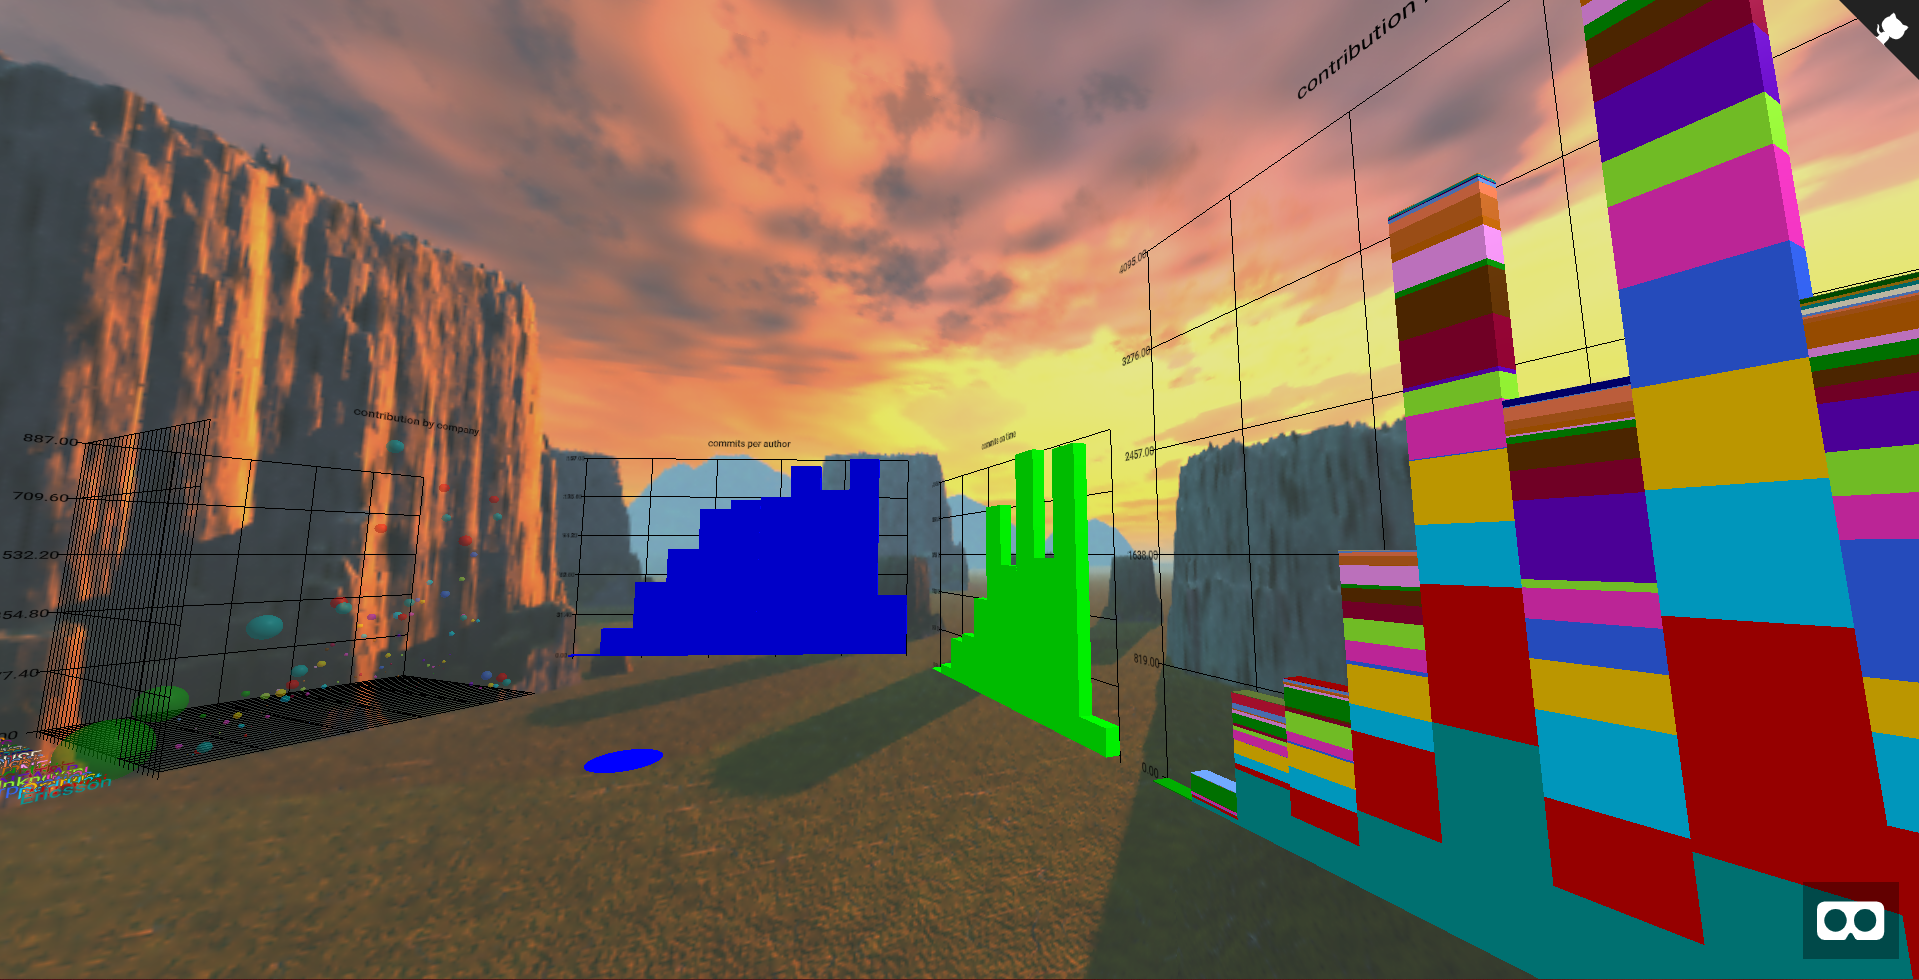
\includegraphics[width=16cm, keepaspectratio]{img/context/aframedc.PNG}
  \caption{Example of charts with A-FrameDC}
  \label{fig:pluginhtml}
\end{figure}



\section{ThreeDC}
\label{sec:threedc}

ThreeDC is library to create different kind of data visualizations based on Three.js\footnote{\url{https://threejs.org/}}. According to the docs that the main developer has, Three.js is a JavaScript library; the aim of the project is to create an easy to use, lightweight, 3D library. The library provides Canvas 2D, SVG, CSS3D and WebGL renderers. It can be defined as "a library to make WebGL easier". 
WebGL is an API. It lets you access a computer’s specialised graphics hardware using JavaScript, and render the output to a webpage in a regular old <canvas> element. Before WebGL, access to that specialised hardware was only really doable with desktop software. The browser was stuck in 2D town (excluding third-party plug-ins such as Adobe Flash).
ThreeDC extiende la API por defecto de Three.js encapsulandola en una nueva API enfocada a la creación de objetos en 3D relacionados con la visualización de datos. De esta manera, se pueden construir este tipo de gráficos en 3D de manera fácil sin tener conocimientos técnicos de Three.js ni WebGL. Esta biblioteca permite la creación de gráficas de líneas en 2D con 2 ejes, barras en 2D y 3D con 2 o 3 ejes (con probabilidad de que sean stacked bars), de burbujas con los 3 ejes y la posibilidad de cambiar el diámetro de estas y pie charts.

This library has been developed by an ex-student of the URJC being his degree thesis\footnote{\url{https://adrianalonsoba.github.io/web-THREEDC/}}.

\begin{figure}[H]
  \centering
  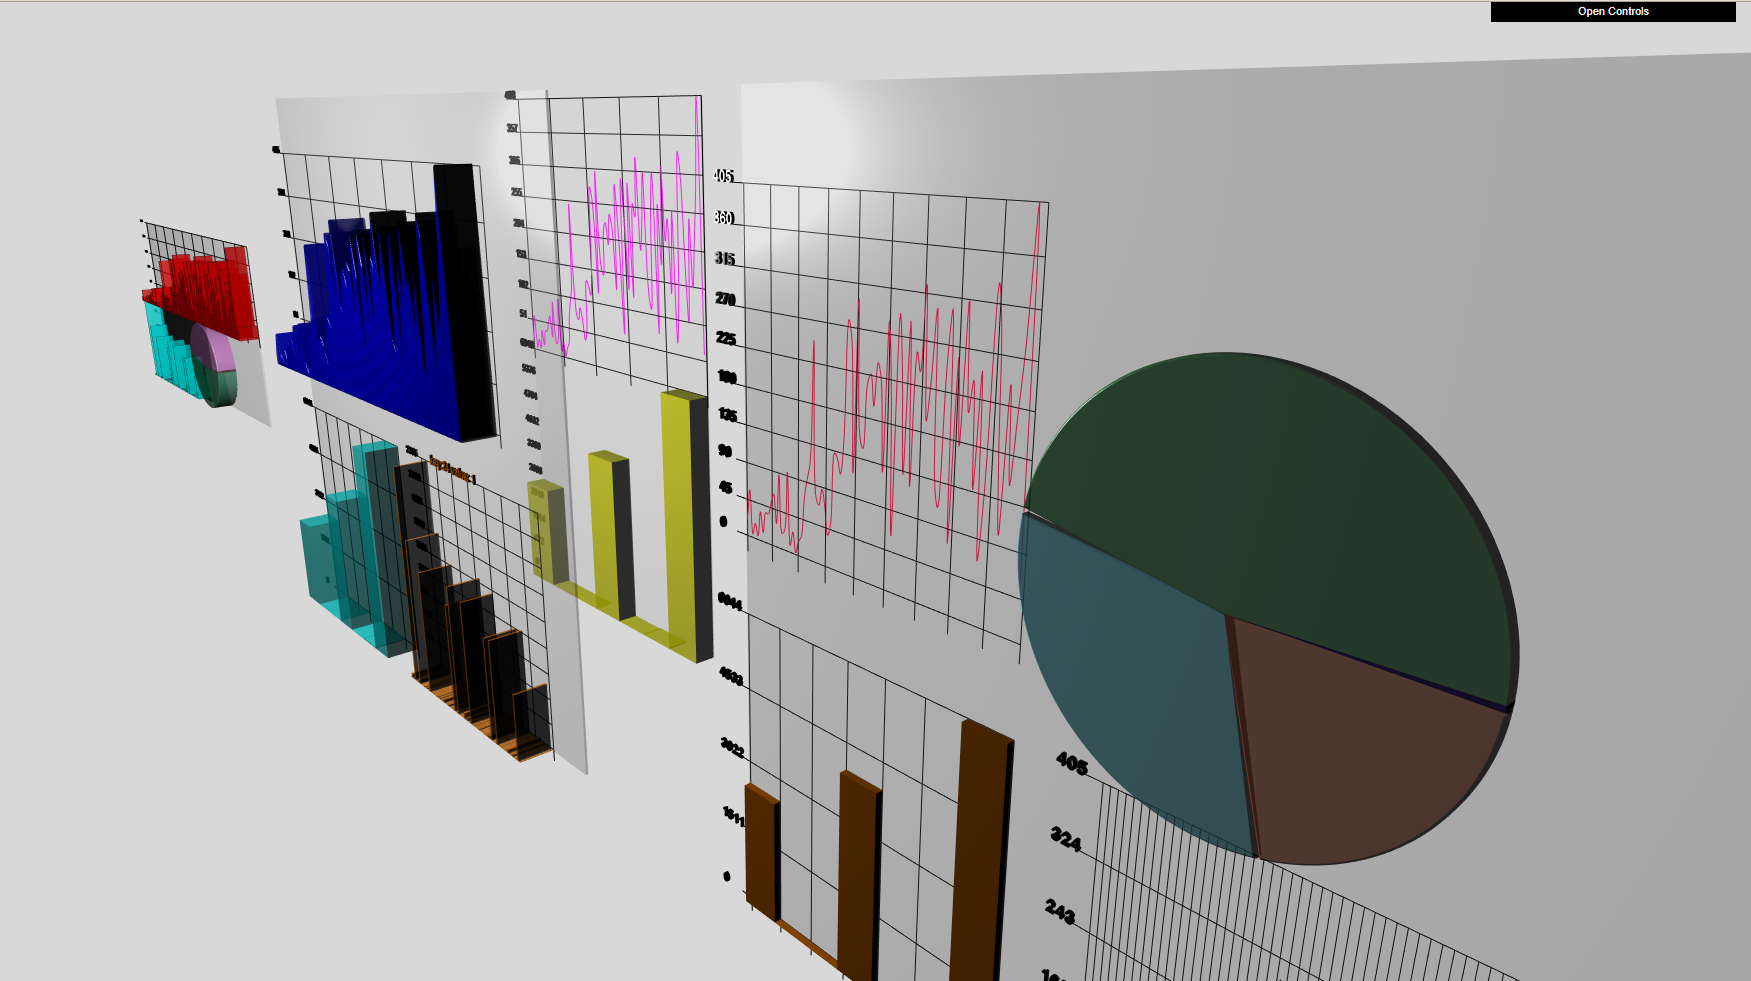
\includegraphics[width=16cm, keepaspectratio]{img/context/threedc.PNG}
  \caption{Example of charts with ThreeDC}
  \label{fig:pluginhtml}
\end{figure}

\section{AngularJS}
\label{sec:angular}
AngularJS is a structural framework for dynamic web apps. It lets you use HTML as your template language and lets you extend HTML's syntax to express your application's components clearly and succinctly. Angular's data binding and dependency injection eliminate much of the code you would otherwise have to write. And it all happens within the browser, making it an ideal partner with any server technology.

AngularJS teaches the browser new syntax through a construct we call directives. Examples include:

\begin{itemize}
\item Data binding, as in \{\{\}\}.
\item DOM control structures for repeating, showing and hiding DOM fragments.
\item Support for forms and form validation.
\item Attaching new behavior to DOM elements, such as DOM event handling.
\item Grouping of HTML into reusable components.
\end{itemize}

AngularJS is not a single piece in the overall puzzle of building the client-side of a web application. It handles all of the DOM and AJAX glue code you once wrote by hand and puts it in a well-defined structure. This makes AngularJS opinionated about how a CRUD (Create, Read, Update, Delete) application should be built. But while it is opinionated, it also tries to make sure that its opinion is just a starting point you can easily change.

AngularJS simplifies application development by presenting a higher level of abstraction to the developer. Like any abstraction, it comes at a cost of flexibility. In other words, not every app is a good fit for Angular. AngularJS was built with the CRUD application in mind. Luckily CRUD applications represent the majority of web applications. To understand what AngularJS is good at, though, it helps to understand when an app is not a good fit for Angular.

Games and GUI editors are examples of applications with intensive and tricky DOM manipulation. These kinds of apps are different from CRUD apps, and as a result are probably not a good fit for Angular. In these cases it may be better to use a library with a lower level of abstraction, such as jQuery.

VBoard is completely written in AngularJS, so it is used all the syntax and optimum ways of the AngularJS development (directives, scopes, modules, etc.).

\section{NodeJS and Npm}
\label{sec:nodejsnpm}
Node.js is a JavaScript runtime built on Chrome's V8 JavaScript engine. Node.js uses an event-driven, non-blocking I/O model that makes it lightweight and efficient.As an asynchronous event driven JavaScript runtime, Node is designed to build scalable network applications.

Node.js applications are written in JavaScript, and can be run within the Node.js runtime on OS X, Microsoft Windows, and Linux. Node.js also provides a rich library of various JavaScript modules which simplifies the development of web applications using Node.js to a great extent.

\begin{lstlisting}[frame=single]
Node.js = Runtime Environment + JavaScript Library
\end{lstlisting}

Following are the areas where Node.js is proving itself as a perfect technology partner.
\begin{itemize}
\item I/O bound Applications
\item Data Streaming Applications
\item Data Intensive Real-time Applications (DIRT)
\item JSON APIs based Applications
\item Single Page Applications
\end{itemize}


Npm (node package manager) is the package manager for JavaScript. Find, share, and reuse packages of code from hundreds of thousands of developers — and assemble them in powerful new ways. 

The best way to manage locally installed npm packages is to create a package.json file.A package.json file affords you a lot of great things:
\begin{enumerate}
\item It serves as documentation for what packages your project depends on.
\item It allows you to specify the versions of a package that your project can use using semantic versioning rules.
\item Makes your build reproducible which means that its way easier to share with other developers.
\end{enumerate}

As a bare minimum, a package.json must have:
\begin{itemize}
\item "name"
\begin{itemize}
\item all lowercase
\item one word, no spaces
\item dashes and underscores allowed
\end{itemize}
\item "version"
\begin{itemize}
\item in the form of x.x.x
\end{itemize}
\end{itemize}

For example:
\begin{lstlisting}[frame=single]
{
  "name": "my-awesome-package",
  "version": "1.0.0"
}
\end{lstlisting}

The installation of the necessary modules to show the visualization will be done by npm, building its own "package.json" inside the plugin directory.  Once the file is built indicating the modules to install, they will be downloaded and installed with the statement "npm install" into a "node\_modules" folder for its later use.

\section{Other Packages Used}
\label{sec:otherspackage}
\subsection{Bodybuilder}
Bodybuilder\footnote{\url{https://bodybuilder.js.org/}} is a small library that makes ElasticSearch queries easier to write, read, and maintain. Esta biblioteca es usada en el proyecto para todas las queries que se hacen a ElasticSearch, de esta manera no es necesario utilizar un algoritmo que construya elJ JSON de la query, simplemente se llaman a métodos más genéricos de esta biblioteca contruyendo el JSON de manera fácil y automática.


\subsection{Bootstrap}
Bootstrap\footnote{\url{https://getbootstrap.com/}} is an open source toolkit for developing with HTML, CSS, and JS. I used for building entire apps with Sass variables and mixins, responsive grid system, extensive prebuilt components, and powerful plugins built on jQuery. Toda la distribución de los elementos HTML y su correspondiente CSS de VBoard están modulados con Bootstrap.

\subsection{RequireJS}
According to the main page, RequireJS\footnote{\url{https://requirejs.org/}} is a JavaScript file and module loader. It is optimized for in-browser use, but it can be used in other JavaScript environments, like Rhino and Node. Using a modular script loader like RequireJS will improve the speed and quality of your code. La incoporación de API's, modulos, servicios de la aplicación VBoard se hace mediante el uso de RequireJS, importando así todo lo necesario.



%%%%%%%%%%%%%%%%%%%%%%%%%%%%%%%%%%%%%%%%%%%%%%%%%%%%%%%%%%%%%%%%%%%%%%%%%%%%%%%%
%%%%%%%%%%%%%%%%%%%%%%%%%%%%%%%%%%%%%%%%%%%%%%%%%%%%%%%%%%%%%%%%%%%%%%%%%%%%%%%%
% DESARROLLO %
%%%%%%%%%%%%%%%%%%%%%%%%%%%%%%%%%%%%%%%%%%%%%%%%%%%%%%%%%%%%%%%%%%%%%%%%%%%%%%%%

\chapter{Development}

In this chapter, we will analyze the use and development of the application from an increasing point of view, guiding the reader through every stage the project has passed, like he/she had developed it him/herself. The development has been carried out increasingly, leading to different kind of prototypes based on the iterations the project has progressed. This format agrees with the methodology SCRUM.

\section{SCRUM methodology}
SCRUM is an iterative and incremental agile software development framework for managing product development. It defines "a flexible, holistic product development strategy where a development team works as a unit to reach a common goal", challenges assumptions of the "traditional, sequential approach" to product development, and enables teams to self-organize by encouraging physical co-location or close online collaboration of all team members, as well as daily face-to-face communication among all team members and disciplines in the project.

A key principle of SCRUM is its recognition that during production processes, the customers can change their minds about what they want and need (often called requirements volatility), and that unpredicted challenges cannot be easily addressed in a traditional predictive or planned manner. As such, SCRUM adopts an empirical approach,accepting that the problem cannot be fully understood or defined, focusing instead on maximizing the team's ability to deliver quickly, to respond to emerging requirements and to adapt to evolving technologies and changes in market conditions.

In SCRUM there are three main roles defined:	

\begin{enumerate}
\item \textbf{Product owner}: The person responsible for maintaining the product backlog by representing the interests of the stakeholders, and ensuring the value of the work the development team does.
\item \textbf{SCRUM master}: The person responsible for the scrum process, making sure it is used correctly and maximizing its benefits.
\item \textbf{Development team}: A cross-functional group of people responsible for delivering potentially shippable increments of product at the end of every sprint.
\end{enumerate}

In our case the product owner and the SCRUM master are represented by the project tutor, so the development team is the project author. Apart from that, we follow the SCRUM methodology faithfully.

A sprint (or iteration) is the basic unit of development in SCRUM. The sprint is a time-boxed effort; that is, it is restricted to a specific duration. The duration is fixed in advance for each sprint and is normally between one week and one month, with two weeks being the most common.

Each sprint starts with a sprint planning event that aims to define a sprint backlog, identify the work for the sprint, and make an estimated commitment for the sprint goal. Each sprint ends with a sprint review and sprint retrospective, that reviews progress to show to stakeholders and identify lessons and improvements for the next sprints.

SCRUM emphasizes working product at the end of the sprint that is really done. In the case of software, this likely includes that the software has been integrated, fully tested and end-user documented.

Sprints or iterations:
\begin{enumerate}
\item \textbf{Iteration 0}: Investigation and preliminary study
\item \textbf{Iteration 1}: Define application structure
\item \textbf{Iteration 2}: First visualizations
\item \textbf{Iteration 3}: Add VBoard state logic into ElasticSearch
\item \textbf{Iteration 4}: Define panels
\item \textbf{Iteration 5}: Dashboards and stand alone mode
\item \textbf{Iteration 6}: Integration with A-frameDC
\item \textbf{Iteration 7}: Customization and optimization
\item \textbf{Iteration 8}: Dockerize application
\end{enumerate}

%\ref{fig:scrum}
\begin{figure}[!htb]
  \centering
  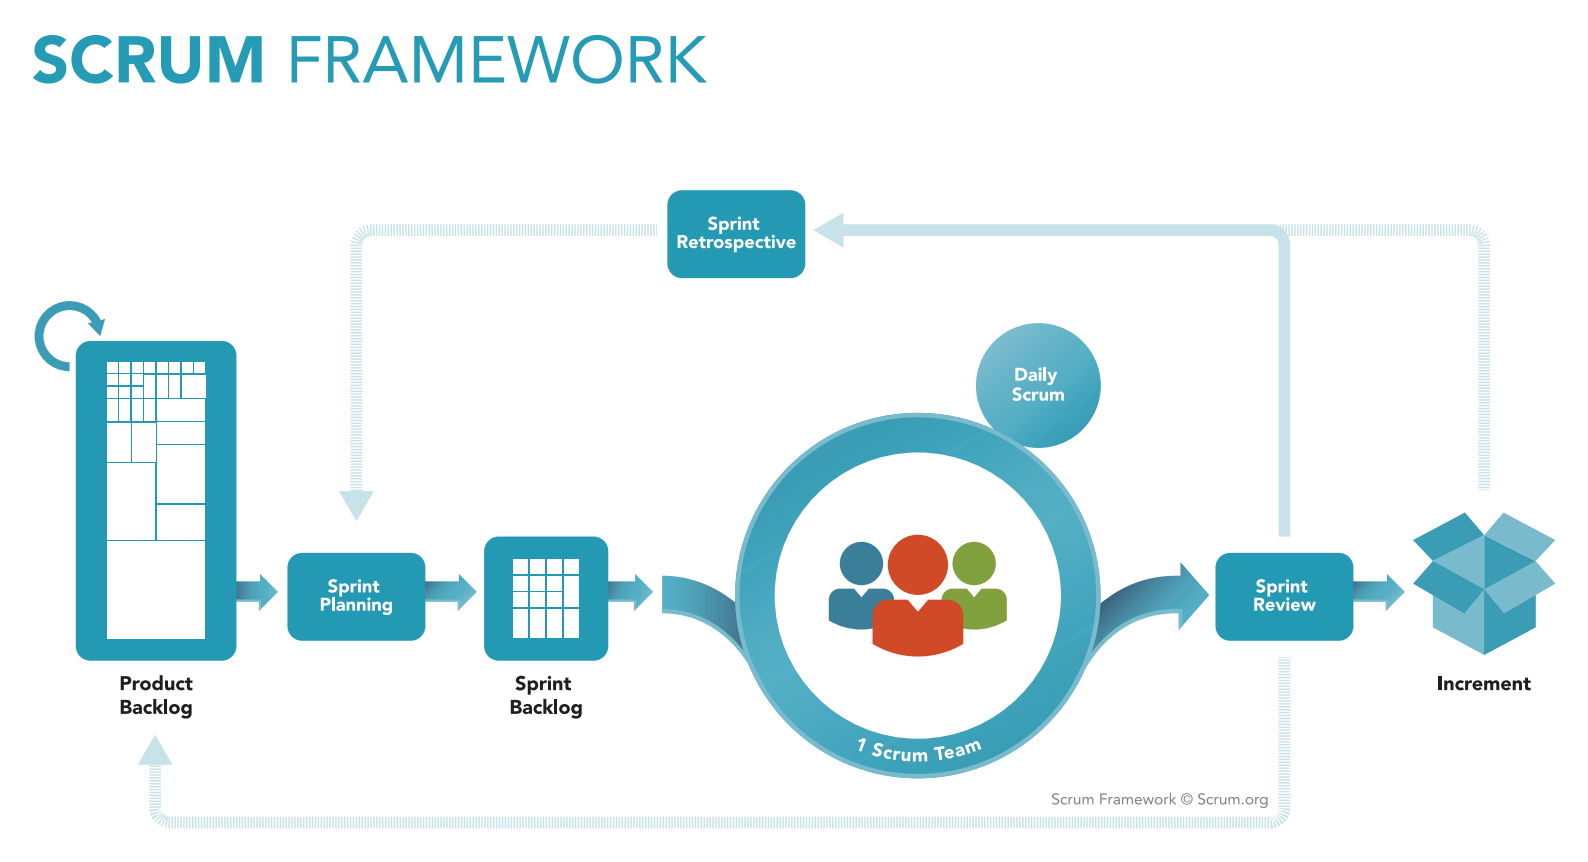
\includegraphics[width=15cm, keepaspectratio]{img/development/SCRUM}
  \caption{The scrum framework}
  \label{fig:scrum}
\end{figure}

\section{Iteration 0: Investigation and preliminary study} 
\label{sec:it0}
This is not an iteration itself, but it is a necessary part of the development, so we decided to include it as 'iteration 0' and here we will get the tools and the study we will need to make our plugin. 

At the beginning, there were a lot of things to explore. First of all, we have to study, understand and get used to ElasticSearch and a framework in order to develop the application.

Durante el desarrollo de este proyecto, me encontraba trabajando en una empresa que utiliza ElasticSearch como base de datos y motor de búsqueda, por lo que la parte de estudio de ElasticSearch ha sido fácil y por lo tanto no se ha necesitado excesivo tiempo para ello. Se ha invertido tiempo en el estudio y análisis de ElasticSearch JS API\footnote{\url{https://www.elastic.co/guide/en/elasticsearch/client/javascript-api/current/api-reference-5-6.html}}, una librería Javascript para manejar las conexiones y hacer todo tipo de peticiones a ElasticSearch.

En el caso de la elección del framework de desarrollo Web, tras la experienza obtenida en el desarrollo del degree thesis (Network Plugin)\footnote{\url{https://dlumbrer.github.io/kbn_network/}} se ha decidido por el uso de AngularJS como framework, ya que se disponen de los conocimientos suficientes para el desarrollo íntegro de la aplicación y por lo tanto el tiempo invertido puede destinarse a futuras funcionalidades de la aplicación.

\section{Iteration 1: Define application structure}
\label{sec:it1}

The aim of this iteration is to define the entire structure, starting with the files structure in order to have isolated each script in a folder that contains scripts with the same type, following the AngularJS standard. Also in this iteration, we are going to define the visual structure, dividing the screen in zones where the items will be, like the menu, the 3D scene, the different pages that it will have, etc.
So we can divide this iteration in this two sub-iterations:

\begin{enumerate}
\item Define the files/scripts structure of the application.
\item Define the visual structure of the application.
\end{enumerate}

\subsection{Files/scripts structure}

To start, la mejor manera de estructurar una aplicación AngularJS, la cual como scripts de primer nivel, o root, tenemos un \textit{index.html} básico con poca información genérica de la aplicación y un \textit{main.js} donde se define la aplicación Angular, como el nombre y el path donde se encuentra el código.

Seguidamente se creará a mismo nivel una carpeta llamada \textit{app/}, otra llamada \textit{templates/} y otra llamada \textit{css/}, en las cuales irán toda la lógica desarrollada para la aplicación. Concretamente dentro de la carpeta \textit{templates/} se encontraran todas las templates html necesarias para la aplicación, todo código HTML5 y con nombres que determinen a que zona/section pertenecen. Dentro de la carpeta \textit{css/} se encontrarán los archivos de estilo para customizar y maquetar el aspecto visual de la aplicación. En la carpeta \textit{app/} se encontrarán toda la lógica JavaScript desarrollada para la aplicación, en su contenido tendrá un script \textit{app\_module.js} donde se instancia la aplicación AngularJS y se define la estructura de esta misma, definiendo los controladores, templates, servicios y directives que necesita. Además, al mismo nivel se encontraran tres tipos de carpetas (si fueran necesarias) donde en su interior, se guardaran los scripts JavaScript correspondientes a las directivas (carpeta \textit{directive/}), los scripts JavaScript correspondientes a los controladores (carpeta \textit{controller/}) y los scripts correspondientes a los servicios externos de la aplicación (carpeta \textit{service/}).

Además, habrá un archivo llamado \textit{package.json} donde se definirá la información (metadata) del proyecto, así como el nombre, el autor, la licencia, y las dependencias NPM que necesita (librerias), por lo tanto, una vez instaladas las dependencias mediante "npm install", estas serán almacenadas dentro de la carpeta \textit{node\_modules/}

Finalmente, existirá otra carpeta con el nombre \textit{js/} donde serán almacenadas aquellas librerias JavaScript que no sean posibles instalar mediante NPM (ThreeDC o A-frameDC por ejemplo) o bien se hayan desarrollado from scratch para este proyecto.

Con esta estructura, el desarrollo es limpio, isolated y fácilmente escalable. La siguiente figura muestra como quedaría finalmente esta estructura:

\begin{figure}[H]
  \centering
  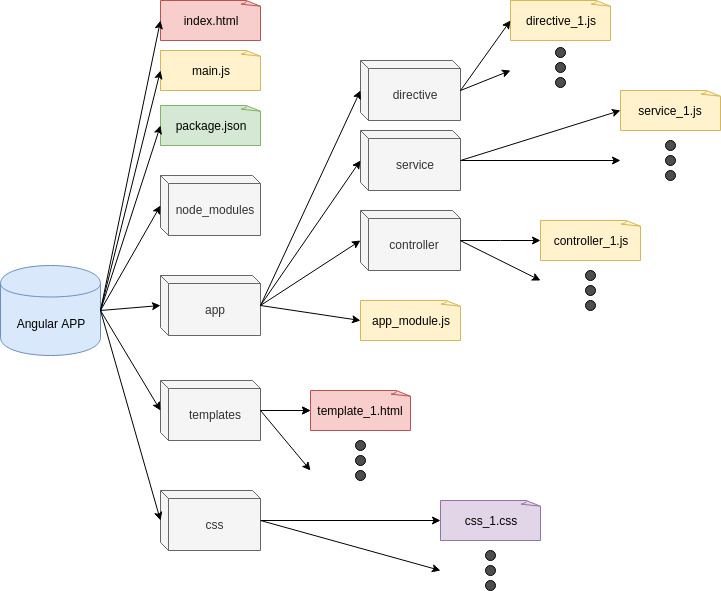
\includegraphics[width=16cm, keepaspectratio]{img/development/Angular_structure}
  \caption{The AngularJS app structure}
  \label{fig:angularjsstructure}
\end{figure}

\subsection{Visual structure}

Para la creacion de dashboards que visualicen datos, nos hemos fijado en aplicaciones como Kibana, Grafana, Freeboard, etc. para seguir un proceso de creación similar y que sea facil y entendible para cualquier usuario. Para ello, el flujo de creación de un dashboard será crear una o varias visualizaciones, opcionalmente crear paneles que contengan una o varias visualizaciones y posteriormente añadir estas visualizaciones a un dashboard, para que finalmente el dashboard contenga toda la información que se quiera visualizar en un entorno de 3D and VR.

\begin{figure}[H]
  \centering
  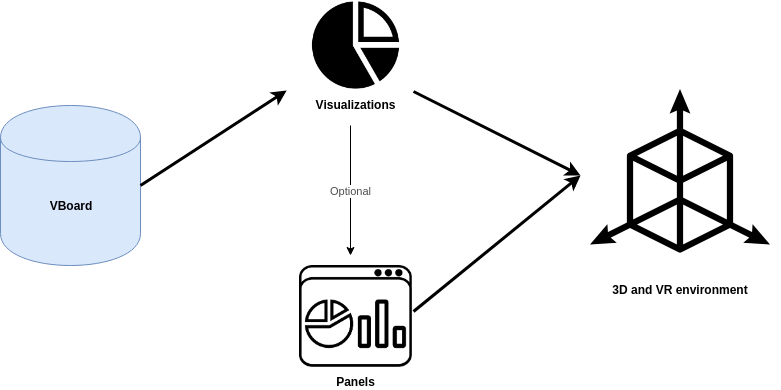
\includegraphics[width=16cm, keepaspectratio]{img/development/Workflow}
  \caption{Create a Dashboard workflow}
  \label{fig:dashboardworkflow}
\end{figure}

Por lo tanto, para seguir este workflow se han definido 3 "tabs" o "areas" en la aplicación: Visualize, Panels, Dashboard and Show:
\begin{enumerate}
    \item \textbf{Visualize}: Sección donde se crearán las visualizaciones, se podrá elegir entre diversos tipos de visualización en 3D y en esta parte también se elgirán que tipos de datos mostrará la visualización. Las visualizaciones podrán guardarse en un futuro con el fin de poder cargarlas/ modificarlas.
    \item \textbf{Panels}: Sección donde se crearán paneles, muros planos externos que contienen visualizaciones, en esta sección se podrá definir el tamaño del panel y el número de visualizaciones que contendrá, además deberán aparecer las visualizaciones disponibles para poder añadirlas al panel. Los paneles podrán guardarse en un futuro con el fin de poder cargarlos/modificarlos.
    \item \textbf{Dashboard}: Sección donde se crearán el "producto" final, un dashboard que será una escena 3D donde se podrán incluir visualizaciones y/o paneles previamente guardados, por lo que deberá aparecer una lista de las visualizaciones/paneles disponibles para poder colocarlos en cualquier parte de las escena, por lo que el usuario deberá elegir en que punto de la escena quiere colocar la visualización/panel y que rotación tendrá. Estos dashboards deben poder guardarse de tal manera que se puedan cargar en otra sección con el fin de visualizarlos, navegar entre ellos y modificarlos.
    \item \textbf{Show}: Esta sección mostrará una lista de dashboards disponibles, cada uno con un enlace a un nuevo recurso en el que solo aparecerñá la escena 3D con un posible botón de VR para poder visualizar el dashboard en modo "stand alone" sin ningún tipo de control en la pantalla, simplemente para observar datos y/o navegar por ellos con VR.
\end{enumerate}

La navegación entre estas tres áreas será mediante una barra de navegación global situada en la parte superior de la aplicación. Esta barra de navegación se mostrará en todas y cada una de las secciones salvo en Show ya que se explicó anteriormente es solamente para visualizar el dashboard sin nada de control alrededor. Además esta barra de navegación se quedara con un "hold" en la sección que se esté en ese momento.

\begin{figure}[H]
  \centering
  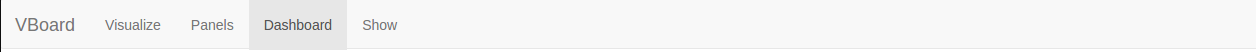
\includegraphics[width=16cm, keepaspectratio]{img/development/navbar}
  \caption{Navbar of VBoard}
  \label{fig:pluginhtml}
\end{figure}

Para el modelado de la estructura visual, se ha usado la biblioteca bootstrap de tal manera que se pueda dividir el contenido fácilmente en filas y columnas de un determinado ancho, de esta manera se ha estructurado el contenido de las secciones Visualize, Panels y Dashboard como un contenido de dos columnas, tal y como se ve en la siguiente imagen:

\begin{figure}[H]
  \centering
  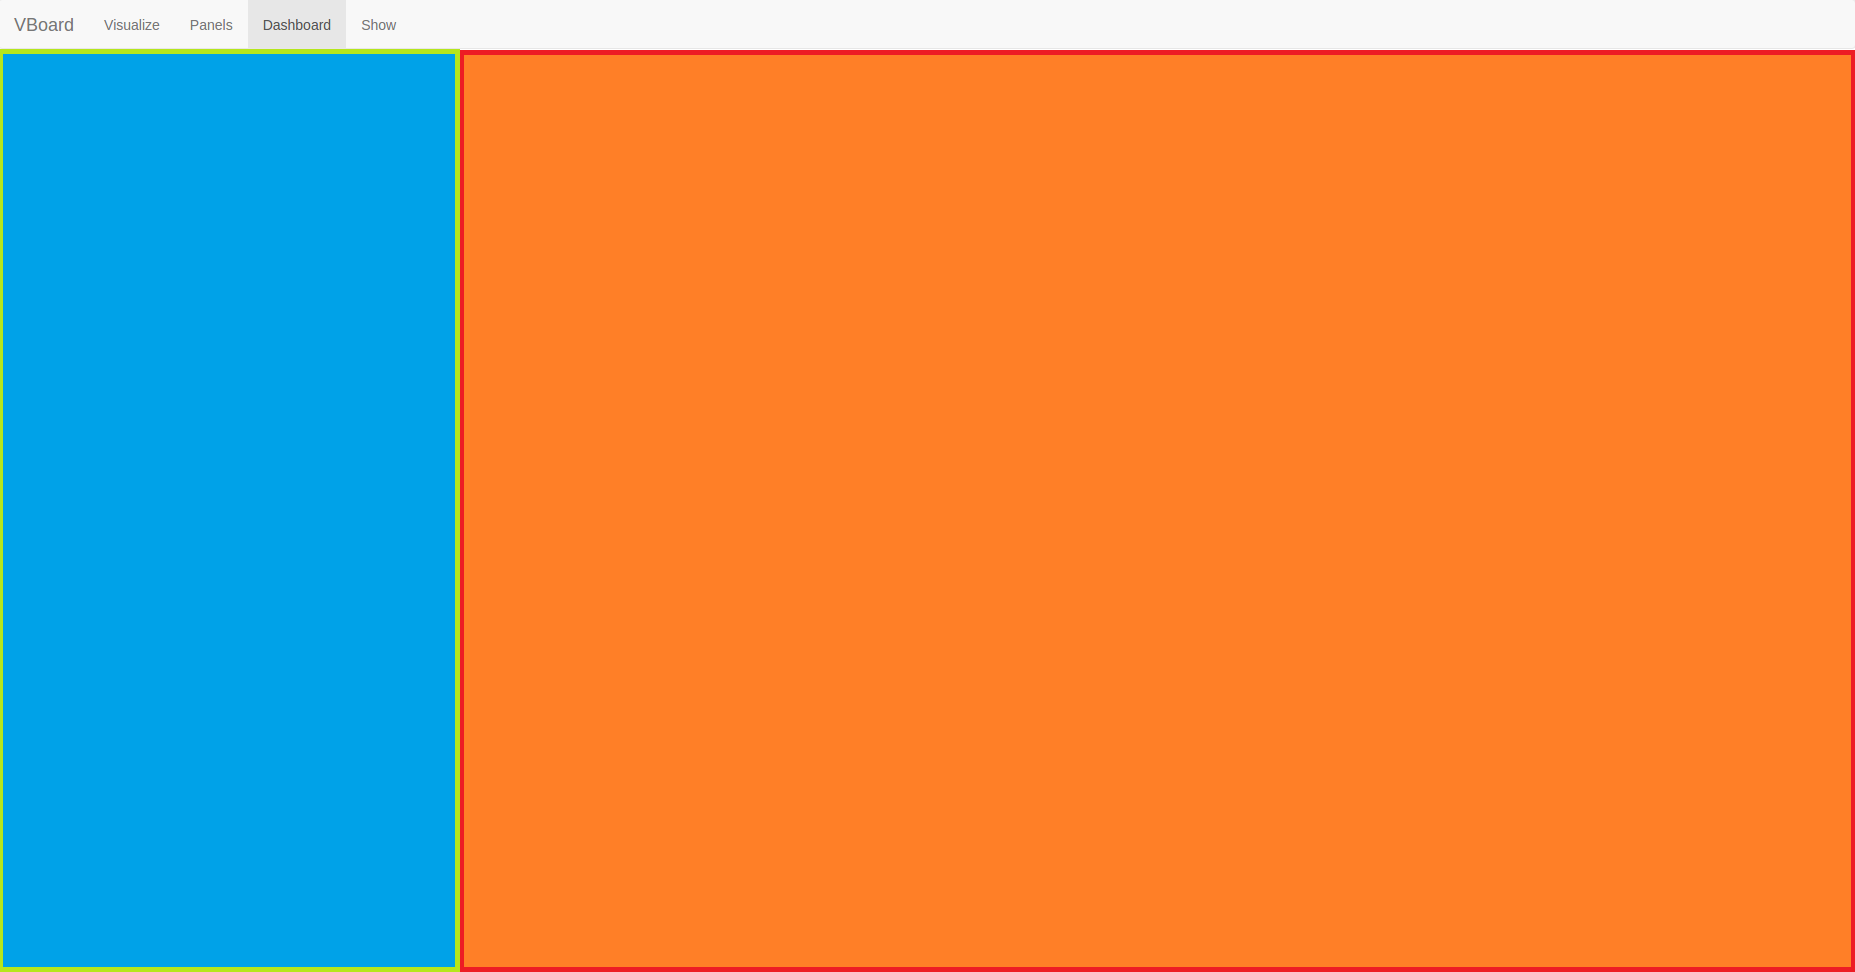
\includegraphics[width=16cm, keepaspectratio]{img/development/visualstructure}
  \caption{Visual Structure of Visualize, Panels and Dashboards}
  \label{fig:pluginhtml}
\end{figure}

La columna de la izquierda, verde y azul de menor tamaño corresponde a la zona de control de la sección, es decir, donde estarán los controles para crear, aportar datos, modificar la visualización/panel/dashboard. La columna naranja correspondrá a la escena 3D donde se visualizarán las visualizaciones/paneles/dashboards. Opcionalmente puede añadirse un botón que cambie a modo VR.

En cambio, la sección Show solo tendrá un contenido en el que irá una lista con los dashboards disponibles, una vez clickado un item de la lista aparecerá una escena en todo el tamaño de la pantalla, sin la barra de navegación ni zona de control:

\begin{figure}[H]
  \centering
  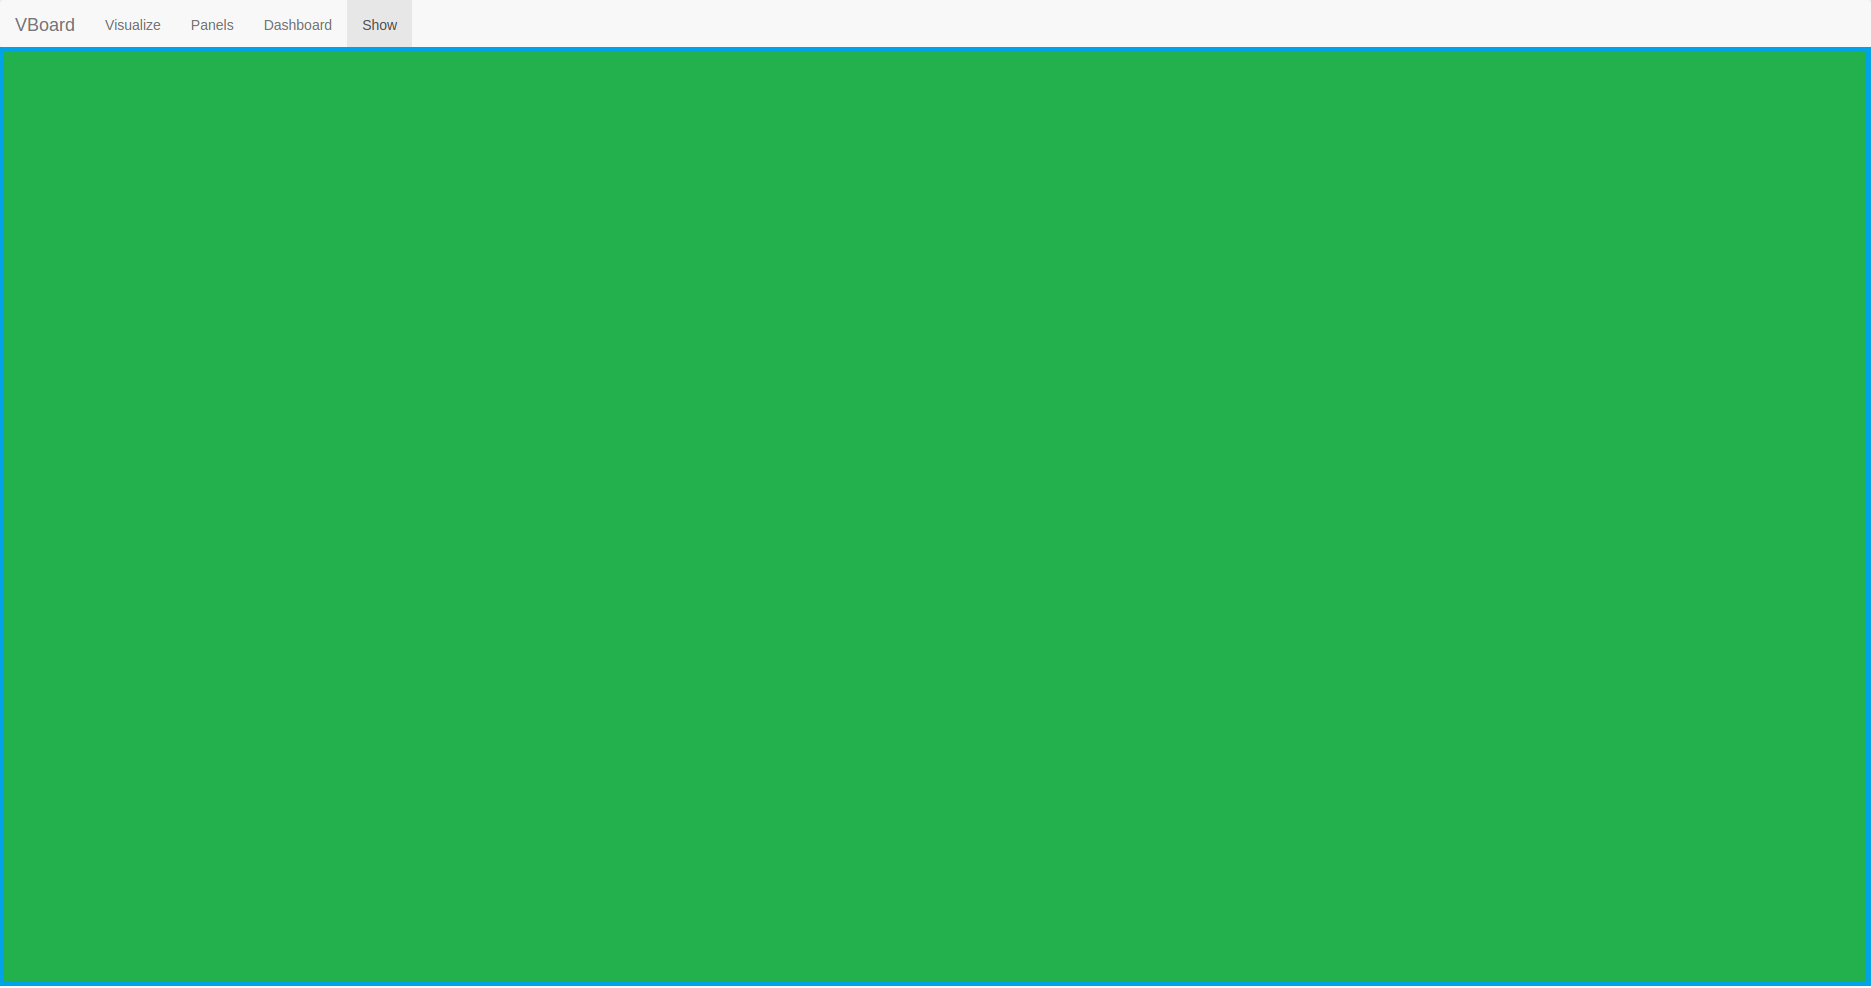
\includegraphics[width=16cm, keepaspectratio]{img/development/showstructure}
  \caption{Visual Structure of Show}
  \label{fig:pluginhtml}
\end{figure}

\section{Iteration 2: First visualizations}

Once we have defined the files structure and developed the visual structure, the next step is to start creating visualizations in the "Visualize" tab for its later integration in a dashboard. Therefore, the aims of this iteration are:

\begin{enumerate}
\item First visualizations without data
\item Integration with ElasticSearch
\item Development of the control menu
\item API's in order to query easy ElasticSearch
\end{enumerate}

\subsection{Visualizations without data}

Para empezar, con el fin de acostumbrarse y saber utilizar la biblioteca ThreeDC, se crearon unas visualizaciones simples en la parte de visualización, sin ningún tipo de datos provenientes de ElasticSearch, se han usado unos datos de prueba que se encontraban directamente en el código, por suerte, el autor de la biblioteca cuenta con varios ejemplos en su web\footnote{https://adrianalonsoba.github.io/web-THREEDC/}, por lo tanto, solo se ha tenido que adaptar estos ejemplos a VBoard. Las siguientes capturas muestran unas de las visualizaciones que se han probado dentro de VBoard:



\begin{figure}[H]
 \centering
  \subfloat[Example of visualizations]{
    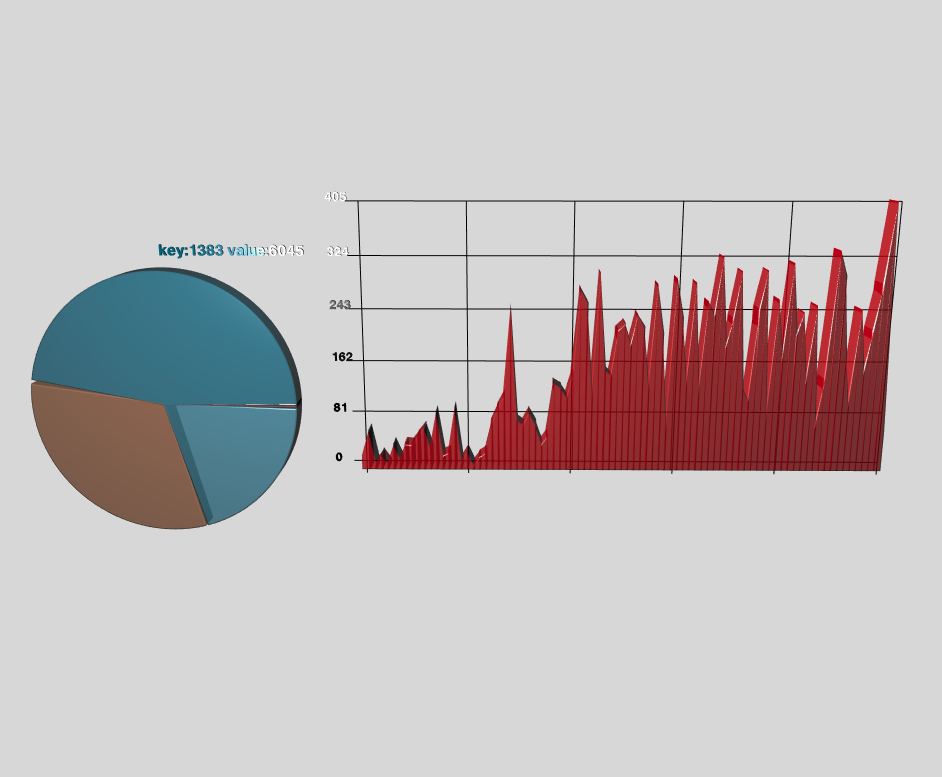
\includegraphics[width=0.5\textwidth]{img/development/example1}}
  \subfloat[Example of panel]{
    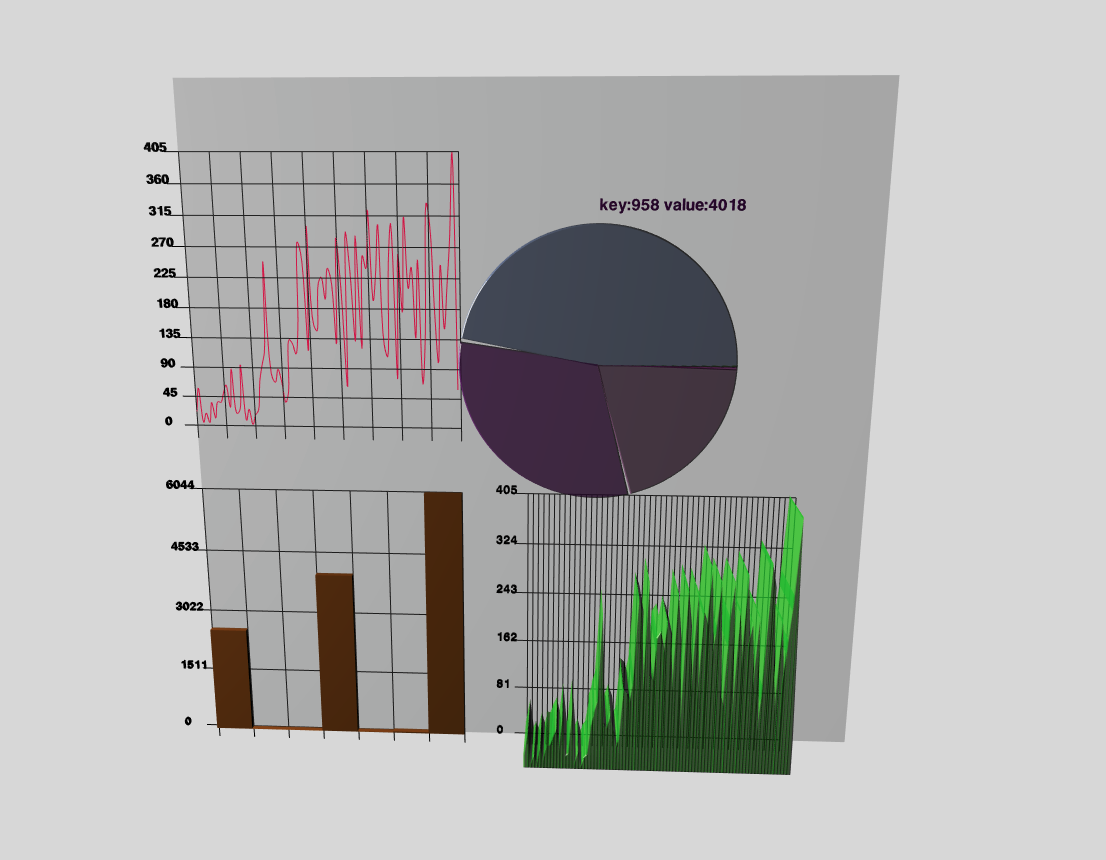
\includegraphics[width=0.5\textwidth]{img/development/example2}}
 \caption{Example of ThreeDC visualizations}
 \label{f:threedcexamples}
\end{figure}

Hay que tener en cuenta que estos ejemplos son simplemente una creacion de una escena añadiendo simples elementos que se pueden crear con ThreeDC, en ninguno de los casos se ha utilizado datos provenientes de un data source, esto será el siguiente objetivo.



\subsection{Integration with ElasticSearch}

Para la integración de ElasticSearch, tal y como se adelantó en la sección \ref{sec:elasticsearch}, se va a utilizar ElasticSearch como base de datos para crear visualizaciones, por lo que en esta aplicación se va a integrar como servicio, creando su archivo \textit{ESService.js} en la correspondiente carpeta \textit{app/service/} de VBoard, dentro de este archivo, se instancia el servicio ElasticSearch, definiciendo un cliente de este dada una dirección, por defecto localhost:9200:

\begin{lstlisting}[frame=single]
define([], function () {
  function ESService(esFactory) {
    this.client = esFactory({
      host: 'http://localhost:9200',
    });
  }
  return ESService;
});
\end{lstlisting}

Con este servicio instanciado, podemos incluir el cliente a ElasticSearch en cualquier controlador que utilicemos en la aplicación, por lo tanto, en el controlador de la pestaña "Visualize" será incluido, de tal manera que podamos crear visualizaciones con datos de ElasticSearch en tiempo real.

Simplemente ya solo podemos realizar queries a ElasticSearch usando este servicio y la API JavaScript que ellos mismos tienen publicada\footnote{\url{https://www.elastic.co/guide/en/elasticsearch/client/javascript-api/current/api-reference-5-6.html}}. El siguiente problema que encontramos fue la construcción de dicha query, la parte que va dentro del body, donde se definen las agregaciones que se van a buscar en ElasticSearch.

Para solucionar este problema se ha utilizado la biblioteca bodybuilder\footnote{\url{https://bodybuilder.js.org/}}, para hacer estas agregaciones y construir el objeto que va dentro de la query de manera sencilla. De todas formas, descubrimos que es mucho código y complejo para usar la biblioteca directamente, por lo que decidimos la creación from scratch dos API's internas, genES y buildES, para realizar las llamadas a ElasticSearch y para crear el objeto que va dentro de la query utilizando bodybuilder.

\subsubsection{buildESDS}
Esta API se encuentra en la carpeta \textit{js/buildESDS.js} y básicamente se encarga de ir guardando las agregaciones elegidas, se compone de pocos métodos, para añadir métricas y buckets, para construir ese objeto (estructura de datos) y para devolverla.

\subsubsection{genES}
Esta API se encuentra en la carpeta \textit{js/genES.js} y esta API se encarga desde crear el objeto que va dentro del body de la query a ElasticSearch utilizando la biblioteca bodybuilder y el objeto de la anterior API (buildESDS) hasta realizar todas las peticiones a ElasticSearch, devolviendo promesas para luego trabajar con los datos devueltos. Es el core de todo lo relacionado con las queries a ElasticSearch. Se compone de varios métodos, desde construir el objeto bodybuilder como de todas las peticiones necesarias.

\subsection{Development of the control menu}

Una vez creadas las API's y todo lo necesario para hacer peticiones a ElasticSearch, el siguiente paso es crear un menu en la zona de control para poder configurar los datos que queramos visualizar así como que tipo de visualización queremos. El menu se ha desarrollado utilizando elementos de bootstrap para que sea useful y tenga una interfaz simple y que cualquier persona pueda entenderla. Por lo tanto, se han definido unos pasos similares a los que tiene la aplicación Kibana para construir una visualización:

\begin{enumerate}
    \item Index and type selection: lo primero es elegir sobre que index and type of our ElasticSearch vamos a querer mostrar los datos, serán dos dropdowns y habrá que elegir primero el de index para poder visualizar algo en de type. Para continuar habría que seleccionar También hay un botón llamado "Show Mapping" para ver opcionalmente el mapping que tiene el índice elegido:
        \begin{figure}[H]
          \centering
          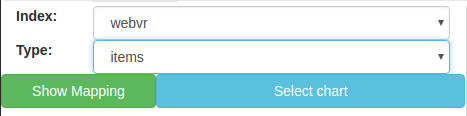
\includegraphics[width=10cm, keepaspectratio]{img/development/indextype}
          \caption{Index/type selection}
          \label{fig:index-type}
        \end{figure}
    \item Visualization type: A dropdown in order to select the different kinds of visualization that will be in VBoard, to continue we have to click on Select Data (or cancel if we want to go back):
        \begin{figure}[H]
          \centering
          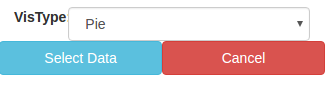
\includegraphics[width=8cm, keepaspectratio]{img/development/vistype}
          \caption{Index/type selection}
          \label{fig:vistype}
        \end{figure}
    \item Select data: Al igual que la aplicación Kibana, aquí es donde se eligen las métricas y buckets que agregarán los datos que se van a mostrar, la cantidad de metricas y buckets necesarios para mostrar la visualización variará dependiendo del tipo de visualización, habrá varios dropdowns para elegir el tipo de métrica/bucket y el campo al que agregará:
    \begin{figure}[H]
      \centering
      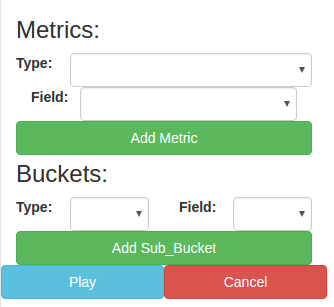
\includegraphics[width=8cm, keepaspectratio]{img/development/aggregationstype}
      \caption{Data selection}
      \label{fig:aggregationstype}
    \end{figure}
\end{enumerate}

Una vez seleccionado todo lo anterior, se pulsará play e internamente, VBoard generará todas las queries y mostrará como resultado la visualización, por ejemplo:

\begin{figure}[H]
  \centering
  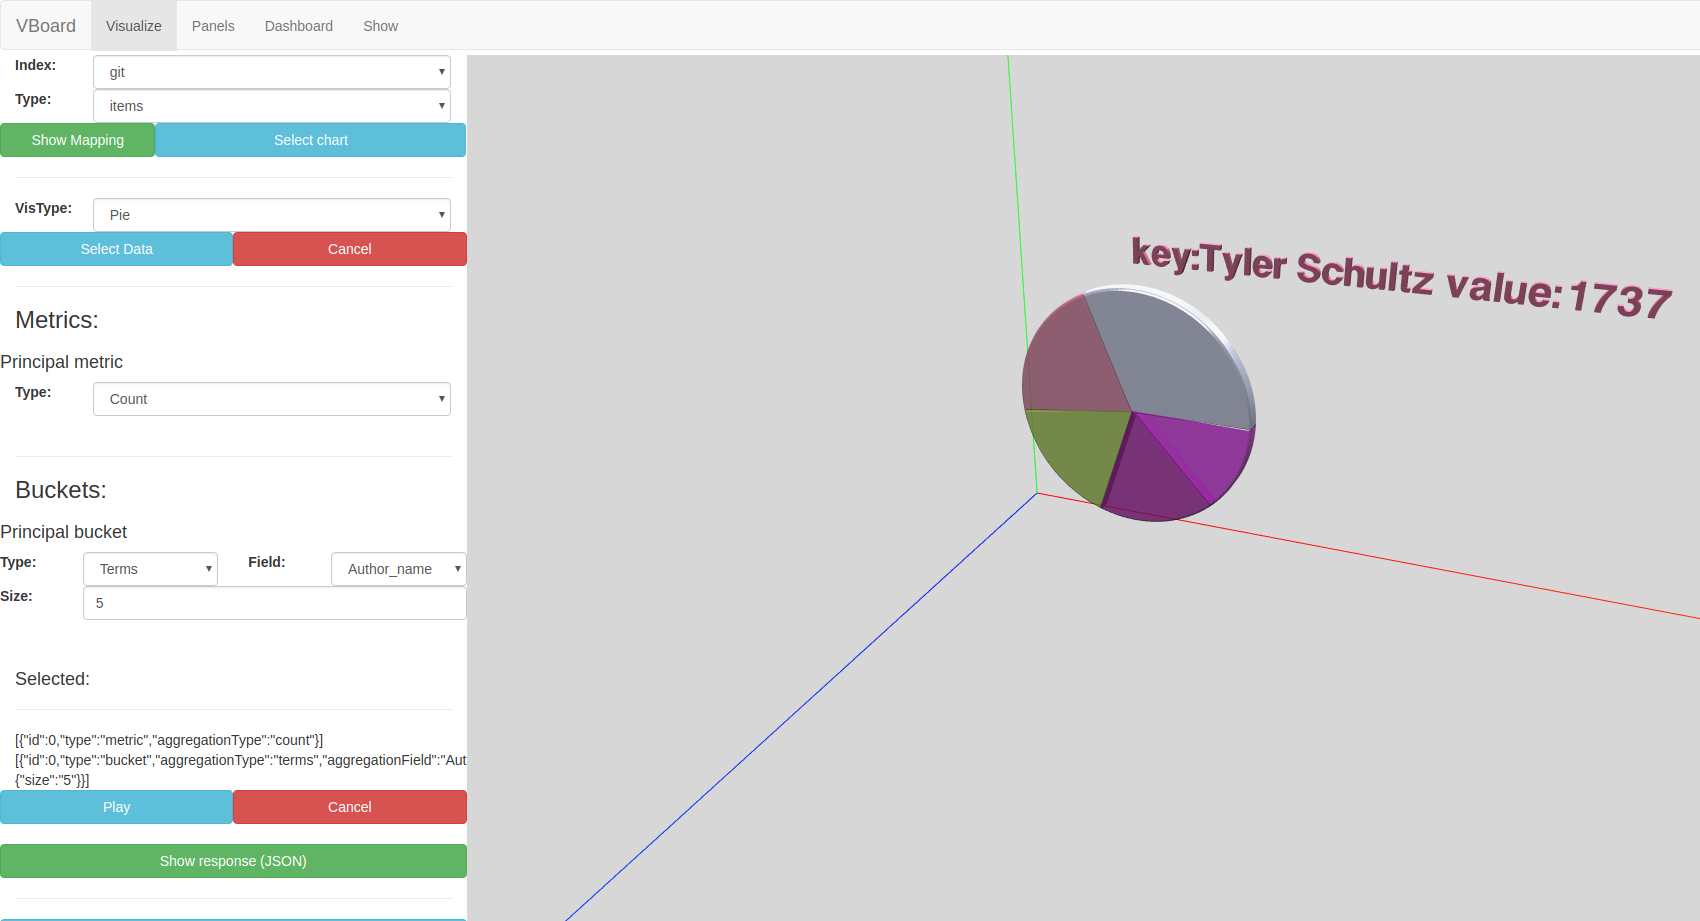
\includegraphics[width=16cm, keepaspectratio]{img/development/firstdatavisualization}
  \caption{First data visualization}
  \label{fig:firsdatavisualization}
\end{figure}

Opcionalmente habrá un botón llamado "Show response (JSON)" de tal manera que se pueda ver el resultado de los datos que se han pedido a ElasticSearch (tanto aggregated como en raw) para mostrar la visualización.


\section{Iteration 3: Add VBoard state logic into ElasticSearch}

El siguiente paso para poder construir paneles y dashboards, es tener una lógica y un sistema de almacenamiento en ElasticSearch para poder guardar nuestras visualizaciones. Para ello, en esta iteracción hemos definido un nuevo índice llamado ".vboard" donde se guardará todo lo relacionado con VBoard. Concretamente en este índice se guardarán las visualizaciones, paneles y dashboards que se hayan creado.

Para definir un índice en ElasticSearch, lo primero que hay que hacer es definir el mapping de tipos y campos que este tendrá, en este caso hemos definido 3 tipos distintos dentro del nuevo índice ".vboard" con el fin de poder tener visualizaciones, paneles y dashboards almacenados en un tipo distinto. Cada documento guardado en cada uno de estos tipos tiene unos campos distintos ya que hay que diferenciar que cada objeto de VBoard es diferente.

Una vez definido las propiedades que quieren almacenarse, el índice de ".vboard" es el siguiente:

\begin{lstlisting}[frame=single]
PUT .vboard
{
    "settings" : {
        "number_of_shards" : 1
    },
    "mappings" : {
        "visthreed" : {
            "properties" : {
                "chartType" : { "type" : "text" },
                "name" : { "type" : "text" },
                "description" : { "type" : "text" },
                "indexOfES" : {"type" : "text"},
                "typeOfES" : {"type": "text"},
                "metricsSelected" : { "type": "object" },
                "bucketsSelected" : { "type": "object" },
                "data" : { "type": "object" }
            }
        },
        "panelthreed" :  {
          "properties": {
                "position" : { "type" : "text" },
                "rows" : { "type" : "text" },
                "columns" : { "type" : "text" },
                "dimension" : { "type" : "text" },
                "opacity" : { "type" : "text" },
                "charts" : { "type" : "object" },
                "name" : { "type" : "text" },
                "description" : { "type" : "text" }
          }
        },
        "dashthreed" : {
            "properties" : {
                "background": { "type": "text"},
                "panels" : { "type" : "object" },
                "charts" : { "type" : "object" },
                "name" : { "type" : "text" },
                "description" : { "type" : "text" }
            }
        }
    }
}
\end{lstlisting}

Toda la lógica de guardado y editado de los elementos de VBoard se ha añadido a la API genES.

En la parte gráfica, se ha desarrollado una lógica para poder guardar las visualizaciones, añadiendo un botón de guardado que abre un "modal" en bootstrap con un formulario para añadir título y descripción a la visualización a guardar:

\begin{figure}[H]
  \centering
  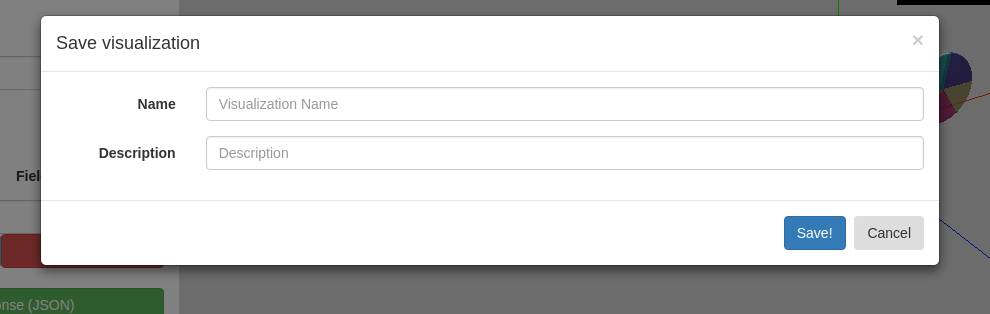
\includegraphics[width=16cm, keepaspectratio]{img/development/examplesave}
  \caption{Form save visualization}
  \label{fig:examplesave}
\end{figure}

De esta manera, la visualziación será guardada con un nombre y descripción. En el caso de que haya una visualización con el mismo nombŕe y tipo aparecerá un formulario preguntando si de verdad queremos sobreescribir la visualización.

Para poder editar una visualización guardada, hemos desarrollado también un botón de carga que muestra una lista de las visualizaciones para cargar:

\begin{figure}[H]
  \centering
  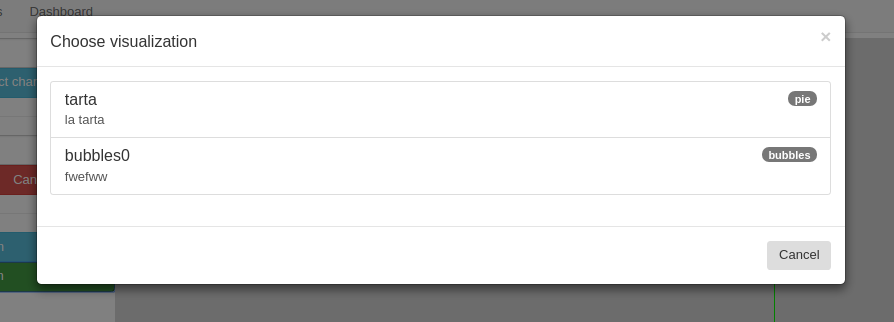
\includegraphics[width=16cm, keepaspectratio]{img/development/exampleload}
  \caption{Form load visualization}
  \label{fig:exampleload}
\end{figure}

Una vez clickeada, se mostrará la visualización con los datos seleccionados para poder editarla o salvarla como una nueva.

\section{Iteration 4: Define panels}

El siguiente paso es definir los paneles, su construcción y posterior save/edit logic. Los paneles es concepto un poco ambiguo, en el entorno de 3D podríamos llamarlo como una "pared" en la cual se "colocan" visualizaciones. Esta implementación la hemos metido ya que el creador de la biblioteca THREEDC lo tiene incluido en su API.

Un panel está definido por ancho, por alto, opacidad y por tamaño de visualizaciones que pueden colocarse en él. Por defecto, aparecerá un panel vacío con una opacidad y tamaño definidos, pero se encontará un botón llamado "New Panel" para poder construirlo from scratch.

Por lo tanto, en el menu de control hay una lista con las visualizaciones disponibles para añadir al panel, mostrando el tipo de visualización que es y su titulo y descripción. Una vez clickado un item, aparece un formulario simple para definir en que lugar del panel quieres colocar la visualización, ya que este se divide por celdas, por lo que hay que seleccionar una fila y columna donde quieras colocar la visualización:

\begin{figure}[H]
 \centering
  \subfloat[Example of visualizations available]{
    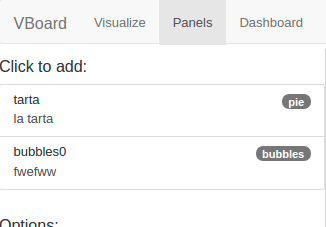
\includegraphics[width=0.3\textwidth]{img/development/panelvislist}}
  \subfloat[Example of add vis to panel form]{
    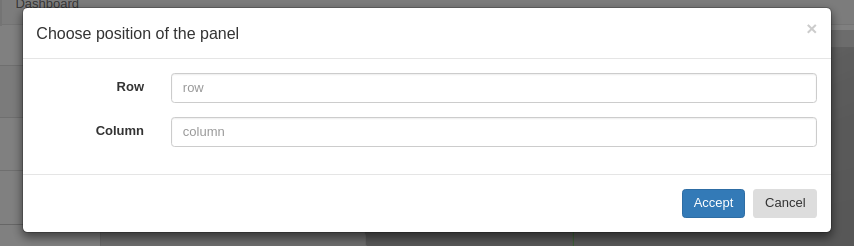
\includegraphics[width=0.7\textwidth]{img/development/exampleaddvistopanel}}
 \caption{Add visualization to a panel}
 \label{f:threedcexamples}
\end{figure}

Debajo de esta lista de visualizaciones disponibles, se encontarán los botones de "New Panel", "Load Panel" and "Save Panel":

\begin{figure}[H]
  \centering
  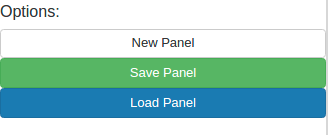
\includegraphics[width=6cm, keepaspectratio]{img/development/panelsbuttons}
  \caption{Options buttons of Panels}
  \label{fig:panelsbuttons}
\end{figure}

Como ya se explicó, al pulsar en "New Panel" se abrirá un nuevo formulario para resetear el panel actual y empezar uno nuevo. Este es el formulario para iniciar un panel con sus características:

\begin{figure}[H]
  \centering
  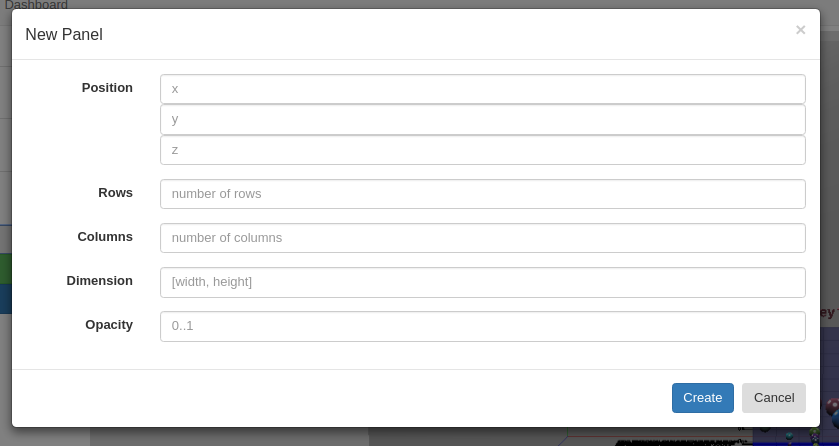
\includegraphics[width=16cm, keepaspectratio]{img/development/newpanelmodal}
  \caption{New Panel Modal}
  \label{fig:newpanelmodal}
\end{figure}

En el caso de clickar en "Save Panel", al igual que en Visualize, se abrirá un modal con un formulario para añadir título y descripción al panel, posteriormente se guardará en ElasticSearch:

\begin{figure}[H]
  \centering
  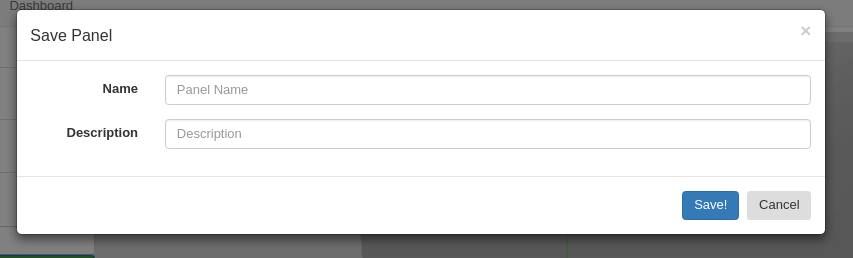
\includegraphics[width=16cm, keepaspectratio]{img/development/savepanelmodal}
  \caption{Save Panel Modal}
  \label{fig:savepanelmodal}
\end{figure}

Y para finalizar, el botón "Load Panel", mostrará otro modal con la lista de paneles guardados disponibles, mostrando el título/descripción y numero de charts que contiene, para poder cargarlos y editarlos, una vez clickeado uno, se cargará él y todo su contenido para su posterior edición o guardado como uno nuevo:

\begin{figure}[H]
  \centering
  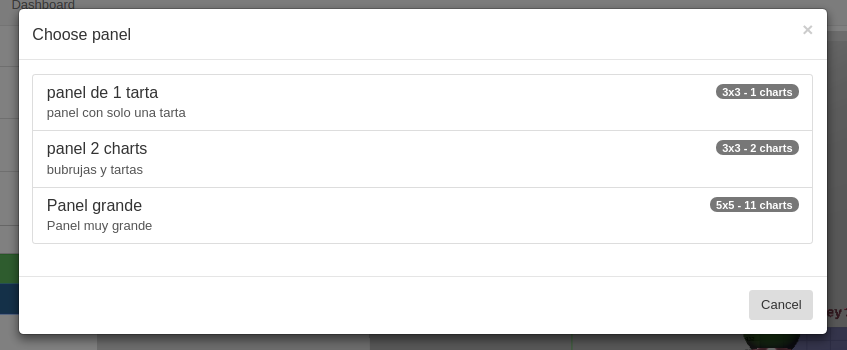
\includegraphics[width=16cm, keepaspectratio]{img/development/loadpanelmodal}
  \caption{Load Panel Modal}
  \label{fig:loadpanelmodal}
\end{figure}

Con todo esto implementado, con sus correspondientes funciones para guardado y cargado en genES, se pasará a desarrollar la pestaña Dashboard.

\begin{figure}[H]
  \centering
  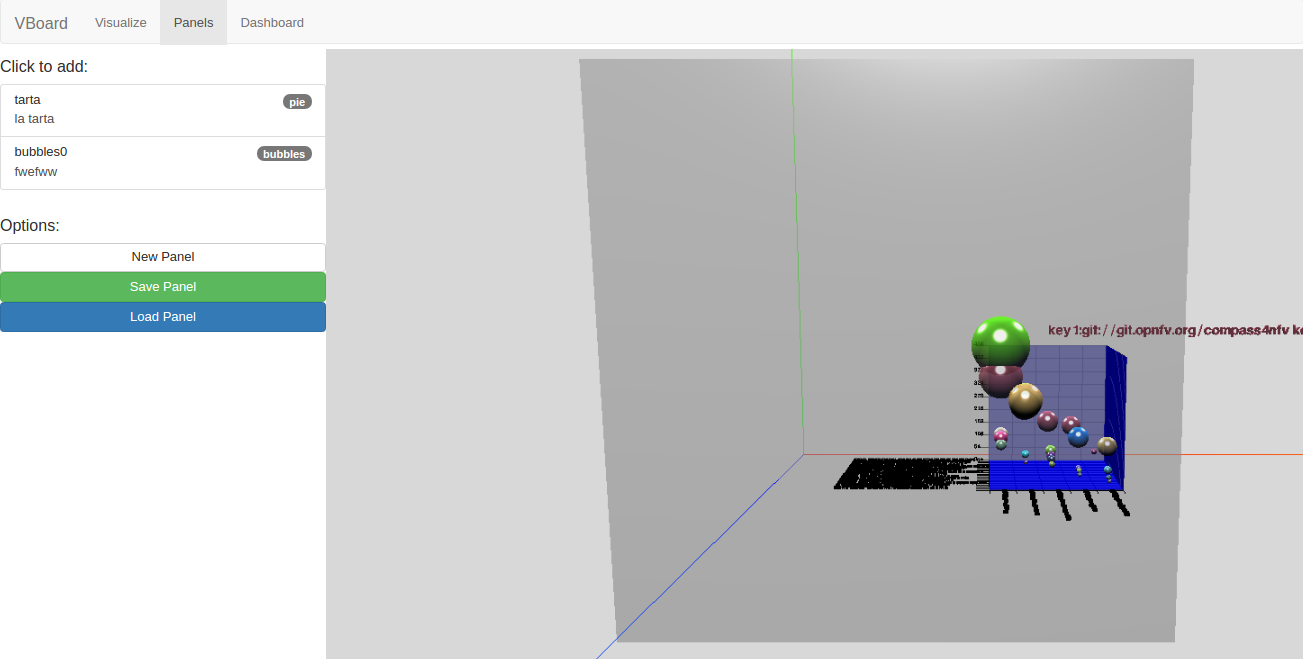
\includegraphics[width=16cm, keepaspectratio]{img/development/examplepanelbubbles}
  \caption{Example of panel with one visualization inside}
  \label{fig:examplepanelbubbles}
\end{figure}

\section{Iteration 5: Dashboard and stand alone mode}

En esta iteration se divide en 2 subiteracciones:

\begin{enumerate}
    \item Define dashboards
    \item Show dashboard in stand alone version
\end{enumerate}

\subsection{Define dashboards}

El proceso de creación de dashboard es como el de panel, debe de haber una lista de elementos que poder añadir, que en este caso son paneles y visualizaciones y se deben poder añadir en cualquier posición de la escena 3D. Por defecto aparecerá una escena vacía sin visualizaciones.

Por lo tanto, en el menu de control hay una lista con las visualizaciones y paneles disponibles para añadir al panel, mostrando el tipo de visualización que es y su titulo y descripción. Una vez clickado un item, aparece un formulario simple para definir en que lugar de la escena quieres colocar el item, ya que este tiene tanto eje "x", "y" y "z", por lo que hay que seleccionar tres posiciones:

\begin{figure}[H]
 \centering
  \subfloat[List of available items]{
    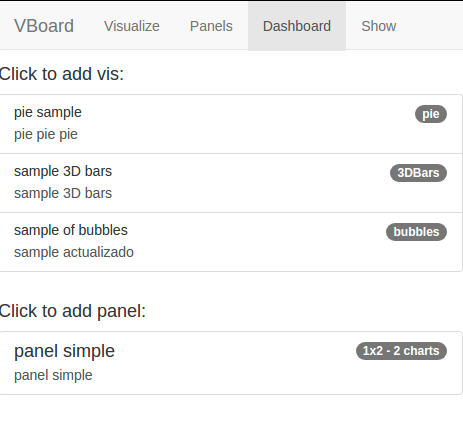
\includegraphics[width=0.3\textwidth]{img/development/addvispaneldashboard}}
  \subfloat[Example of add vis/panel to dashboard form]{
    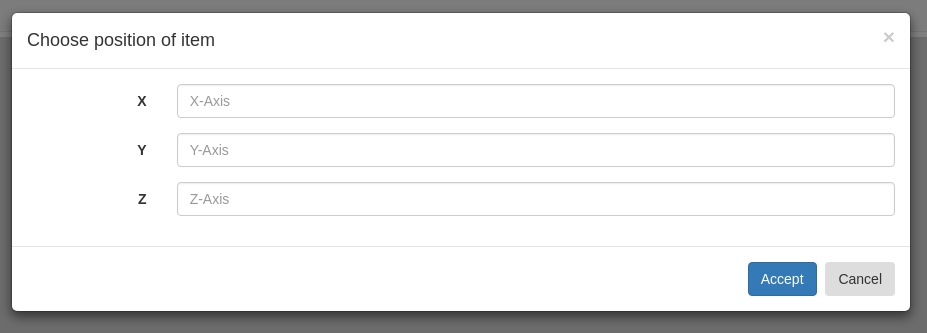
\includegraphics[width=0.7\textwidth]{img/development/exampleaddvistodash}}
 \caption{Add visualization or panel to a dashboard}
 \label{f:threedcexamples}
\end{figure}

Debajo de esta lista de visualizaciones y paneles disponibles, se encontarán los botones de "Save Dashboard" y "Load Dashboard":

\begin{figure}[H]
  \centering
  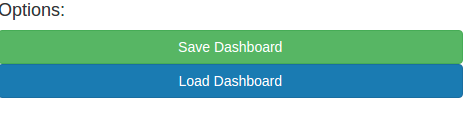
\includegraphics[width=6cm, keepaspectratio]{img/development/dashbuttons}
  \caption{Options buttons of Dashboard}
  \label{fig:dashbuttons}
\end{figure}

En el caso de clickar en "Save Dashboard", al igual que en Visualize, se abrirá un modal con un formulario para añadir título y descripción al dashboard, posteriormente se guardará en ElasticSearch:

\begin{figure}[H]
  \centering
  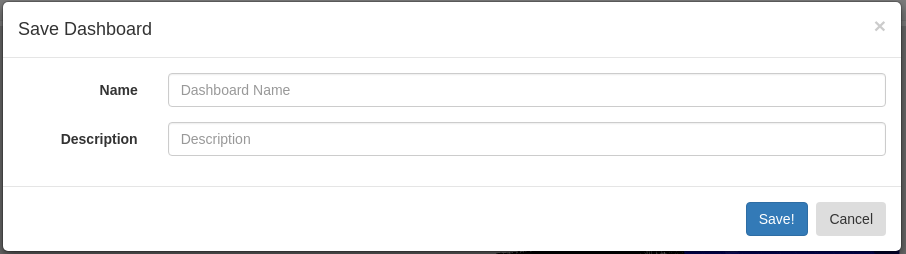
\includegraphics[width=16cm, keepaspectratio]{img/development/examplesavedash}
  \caption{Save Dashboard Modal}
  \label{fig:examplesavedash}
\end{figure}

Y para finalizar, el botón "Load Dashboard", mostrará otro modal con la lista de dashboards guardados, mostrando el título/descripción y numero de charts y paneles que contiene, para poder cargarlos y editarlos, una vez clickeado uno, se cargará él y todo su contenido para su posterior edición o guardado como uno nuevo:

\begin{figure}[H]
  \centering
  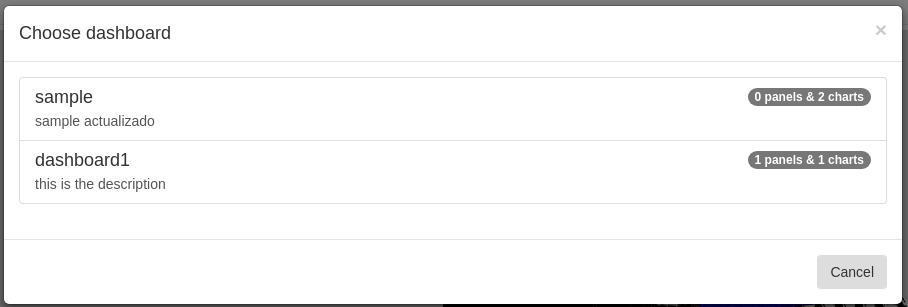
\includegraphics[width=16cm, keepaspectratio]{img/development/exampleloaddash}
  \caption{Load Dashboard Modal}
  \label{fig:exampleloaddash}
\end{figure}

Con todo esto implementado, con sus correspondientes funciones para guardado y cargado en genES, se pasará a desarrollar la pestaña Show.

\begin{figure}[H]
  \centering
  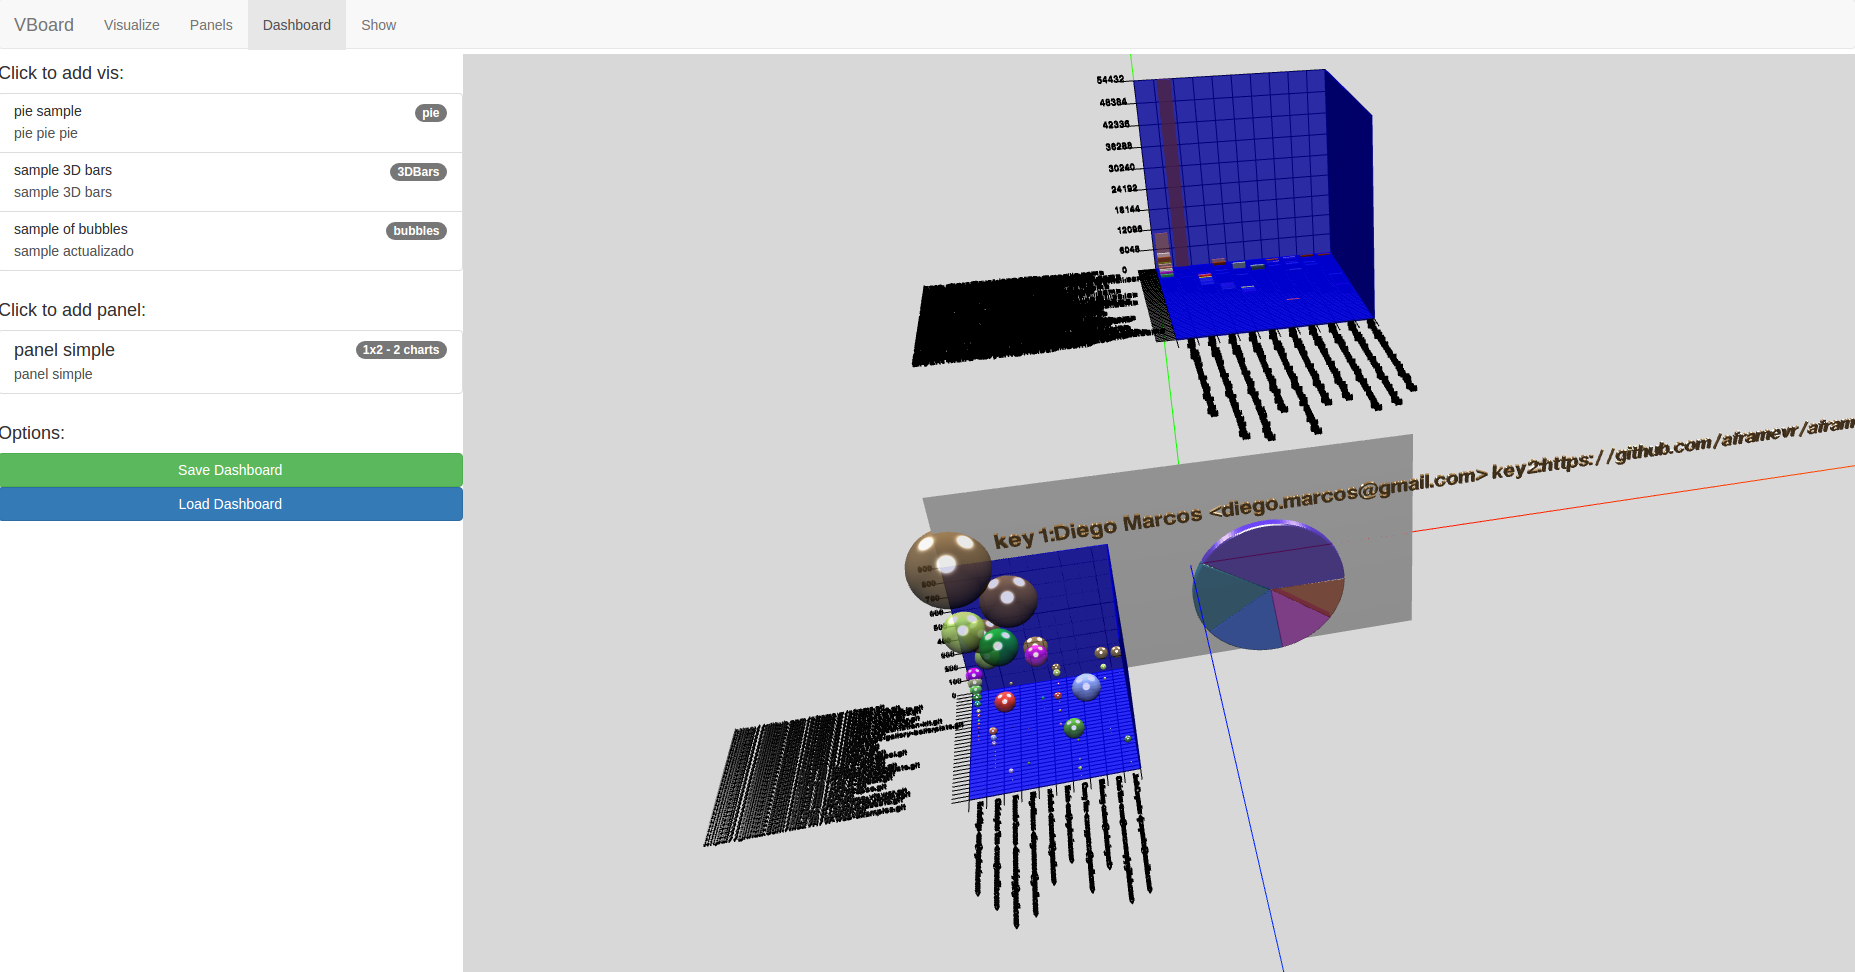
\includegraphics[width=16cm, keepaspectratio]{img/development/exampledashboard}
  \caption{Example of dashboard with one visualization and one panel inside}
  \label{fig:exampledashboard}
\end{figure}

\subsection{Show dashboard in stand alone version}

Para que el usuario pueda visualizar el dashboard de una manera simple y que además no tenga ningún menú en la pantalla, es decir, que solo vea la escena 3D en toda la pantalla y pueda acceder al VR de manera simple, se va a desarrollar una nueva pestaña llamada "Show" que mostrará la lista de dashboards guardados, con el número de paneles y charts que contiene, y una vez clickeado uno, se redirigirá al usuario a una página limpia donde solo se encuentre el dashboard.

Por lo tanto la pestaña show solo tendrá una lista de contenido:

\begin{figure}[H]
  \centering
  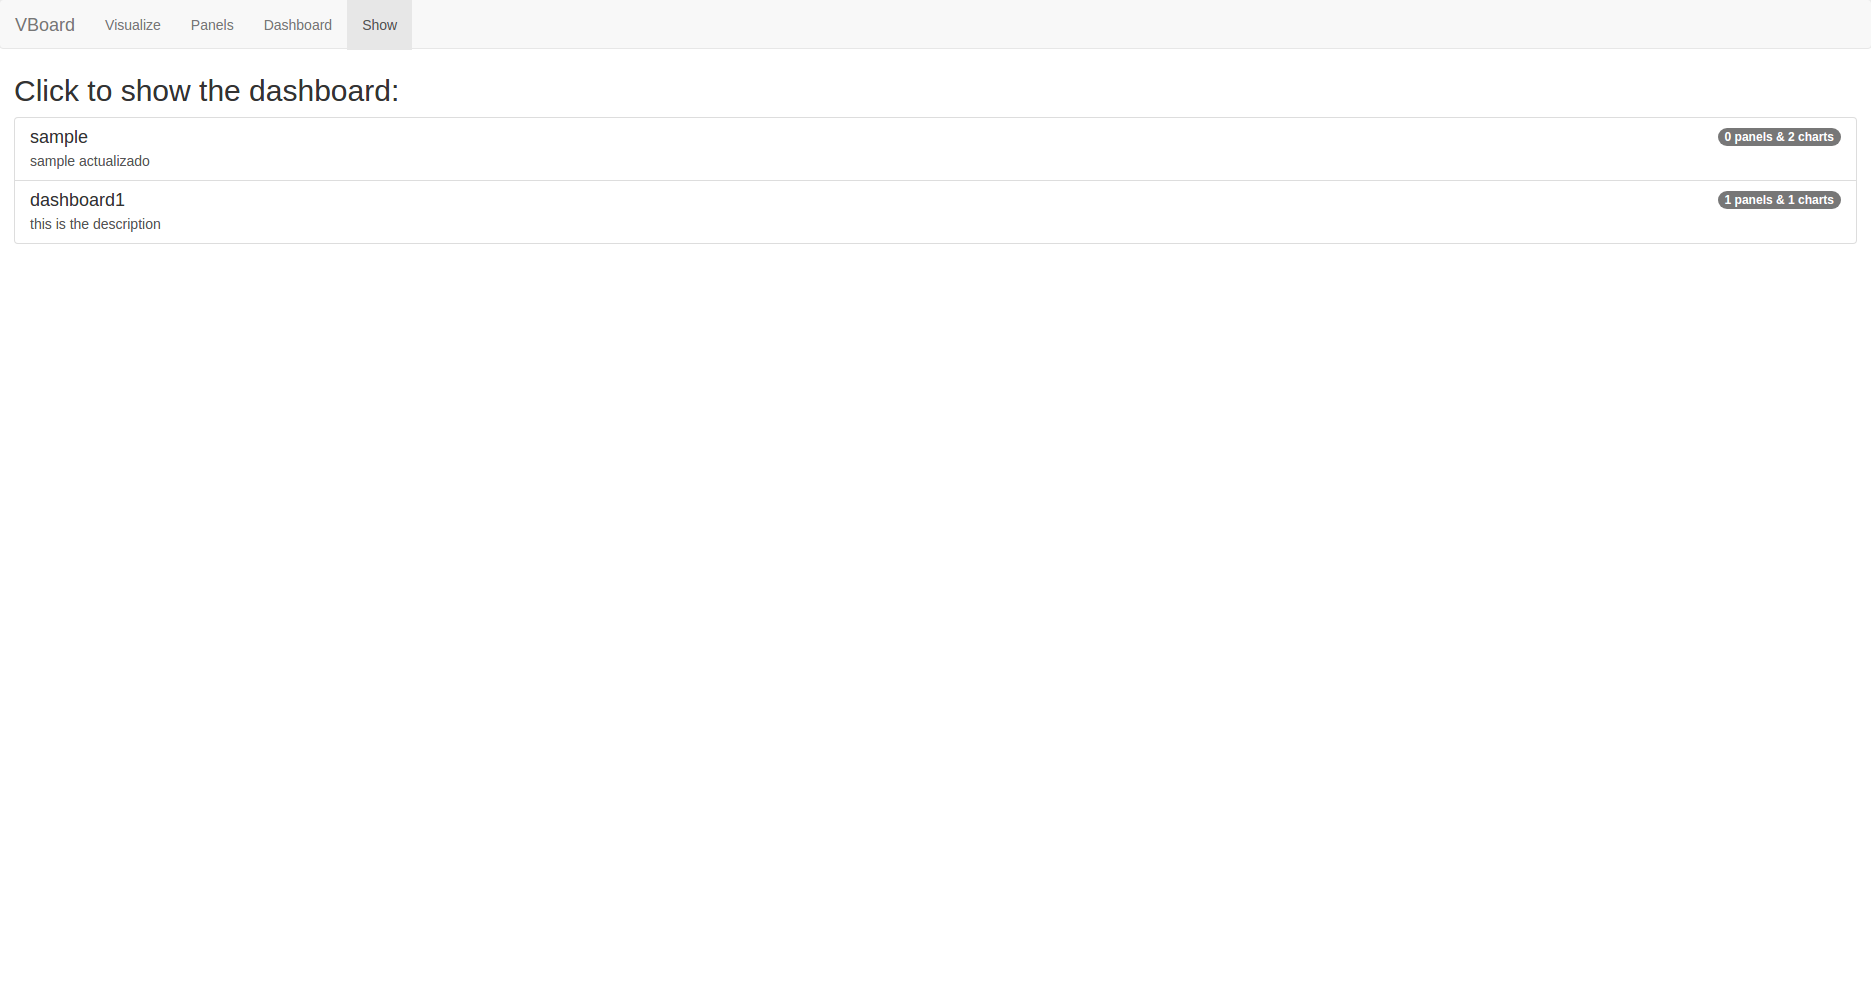
\includegraphics[width=16cm, keepaspectratio]{img/development/exampleshow}
  \caption{Example of the list in Show tab}
  \label{fig:exampleshow}
\end{figure}

Y una vez clickado el contenido, el usuario es redirigido a una url única, de esta manera si el usuario solo quiere acceder al dashboard en modo stand alone, puede acceder con la url sin pasar por los menús de creación: \textit{ localhost:8080/\#!/Show/dashboard\_name}

\begin{figure}[H]
  \centering
  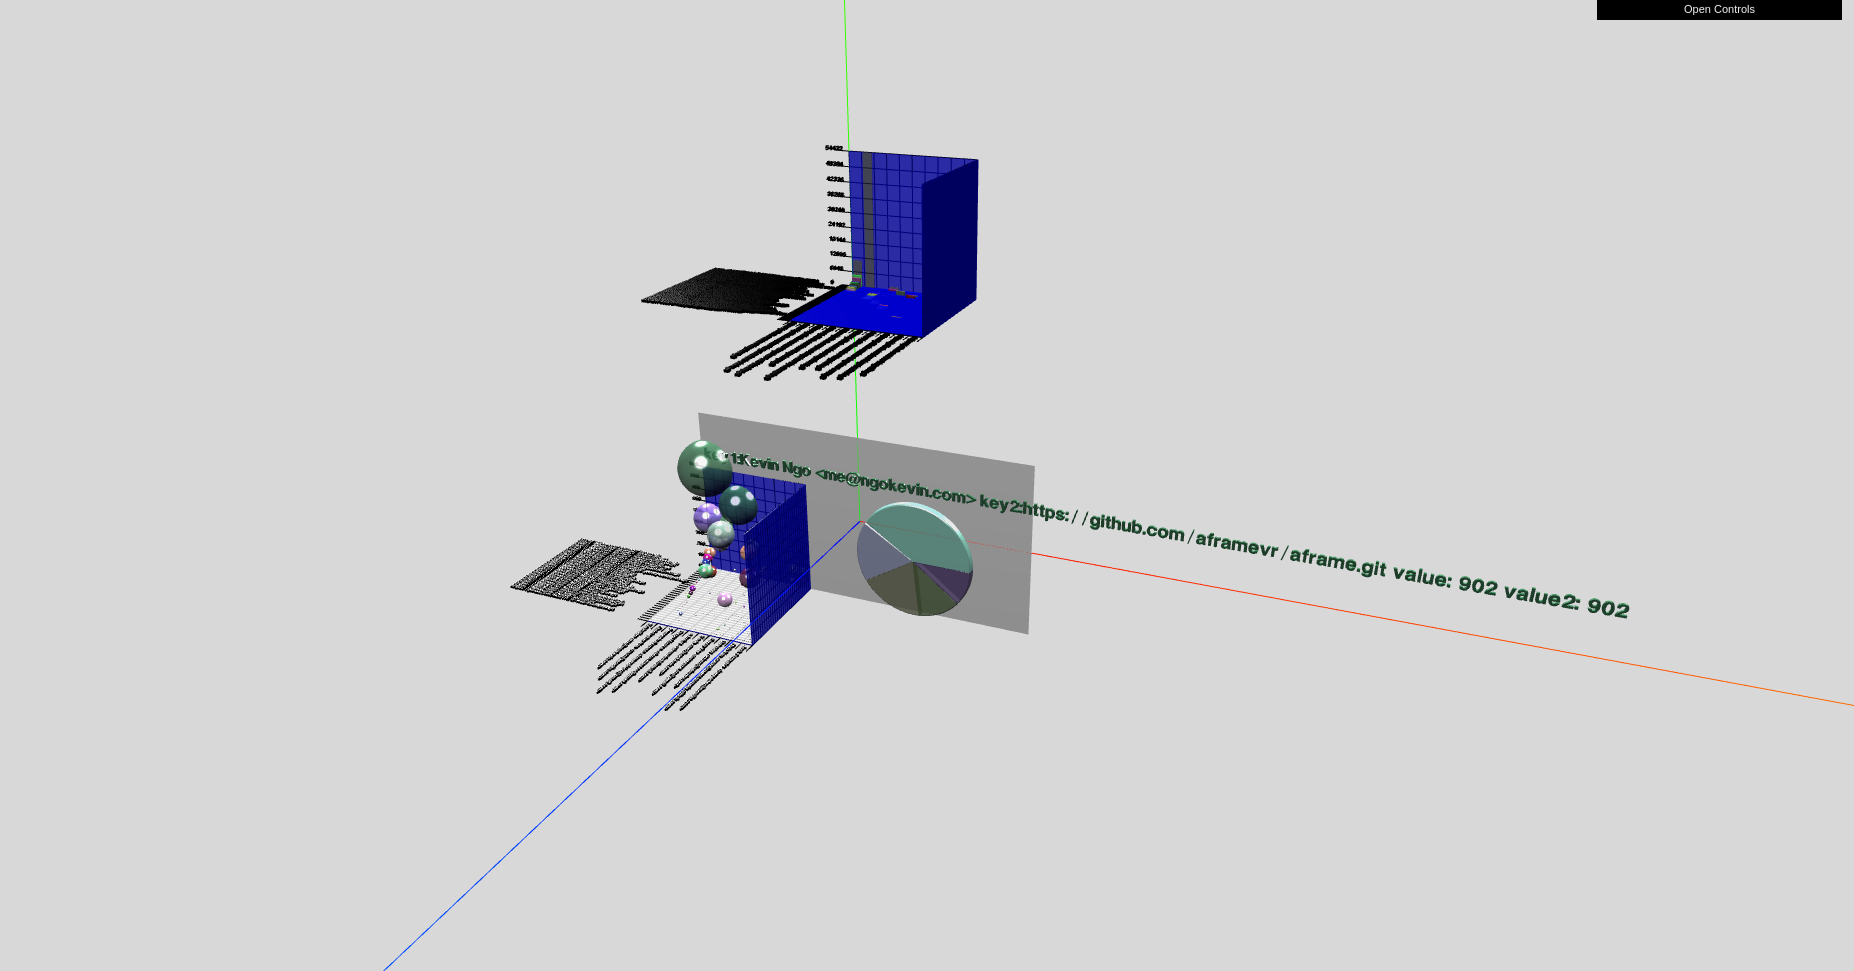
\includegraphics[width=16cm, keepaspectratio]{img/development/examplestandalone}
  \caption{Example of a Dashboard in stand alone mode}
  \label{fig:examplestandalone}
\end{figure}


La aplicación base VBoard está completa, los siguientes pasos serán de mejora de la misma.

\section{Iteration 6: Integration with A-frameDC}

En el medio del desarrollo del proyecto, un antiguo alumno de la universidad presentó una librería JavaScript para la visualización de datos en 3D y VR, A-FrameDC\footnote{\url{https://fran-aguilar.github.io/a-framedc/}}, al igual que ThreeDC pero utilizando A-Frame como motor de renderizado (his degree thesis). A partir de este momento, este proyecto cambió abruptamente, decidimos incluir esta nueva biblioteca, ya que A-Frame es una biblioteca nueva, en continua evolución, desarrollada por un equipo bastante importante en la comunidad (Mozilla) y además es open source. Por lo tanto, esta biblioteca sería incluida en VBoard, llevando un desarrollo en paralelo de dos versiones, la versión con ThreeDC y la version con A-FrameDC.

Las diferencias entre estas dos bibliotecas son mínimas, ambas tienen los mismo métodos para construir visualizaciones en 3D, pero hay que destacar las siguientes diferencias que nos encontramos al incluirla:

\begin{itemize}
    \item A-FrameDC al usar A-Frame como motor de renderizado incluye la incoporación de VR de manera nativa, algo que no tiene desarrollado aún ThreeDC, por lo que nos ahorraría mucho tiempo para la implementación de la Realidad Virtual en la Aplicación.
    \item A-FrameDC no tiene la funcionalidad de "Panels", por lo que es imposible construir paneles con esta biblioteca. Igualmente, el concepto de panel en 3D no tiene mucho sentido, por lo que este punto no sería demasiado negativo.
    \item A-Frame no cuenta con el desarrollo de la visualización de Línea en 2D, pero cuenta con la visualziación de smooth curve que es una curva.
\end{itemize}

Tras estos pros y contras, el product owner y el equipo de desarrollo decidimos que nos centraríamos en esta biblioteca ya que es novedosa y más potente que ThreeDC.

\subsection{Modifications to VBoard}

Como se ha comentado en el apartado anterior, no hay que hacer ningún cambio significativo a la aplicación, ya que los métodos de A-FrameDC y ThreeDC son los mismos, lo único que hubo que cambiar es el nombre del objeto que devuele la API al instanciarla (instantiate).

El siguiente paso es eliminar la posibilidad de  el apartado "Panels" de la aplicación, para esto simplemente hay que modificar las librerias genES y el front-end para no guardar la lógica de paneles en ElasticSearch y para no mostrar la pestaña de "Panels" en la aplicación. Una vez eliminada la funcionalidad la aplicación quedaría de la siguiente manera:

\begin{figure}[H]
  \centering
  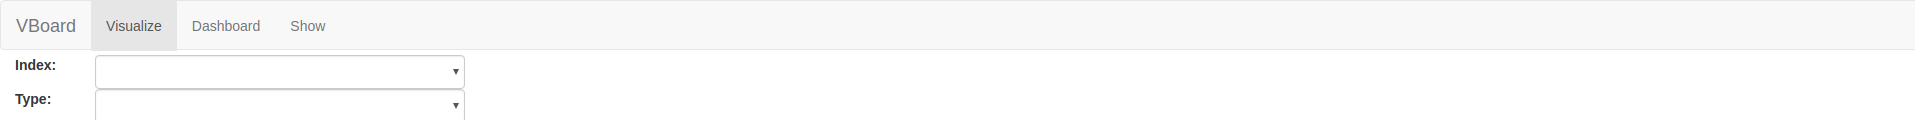
\includegraphics[width=16cm, keepaspectratio]{img/development/newnavbar}
  \caption{New navigation bar with A-FrameDC}
  \label{fig:examplestandalone}
\end{figure}

Además, el punto más positivo de utilizar A-FrameDC es la incoporación nativa de VR, en todas las escenas creadas con A-Frame existe un botón en la esquina inferior derecha que permita activar esta realidad virtual.

\begin{figure}[H]
  \centering
  
\includegraphics[width=4cm, keepaspectratio]{img/development/vrbutton}
  \caption{VR button of A-frame}
  \label{fig:examplestandalone}
\end{figure}

Las siguientes imágenes muestrán unos ejemplos de construcción de visualizaciones y dashboards con VBoard y esta biblioteca:

\begin{figure}[H]
  \centering
  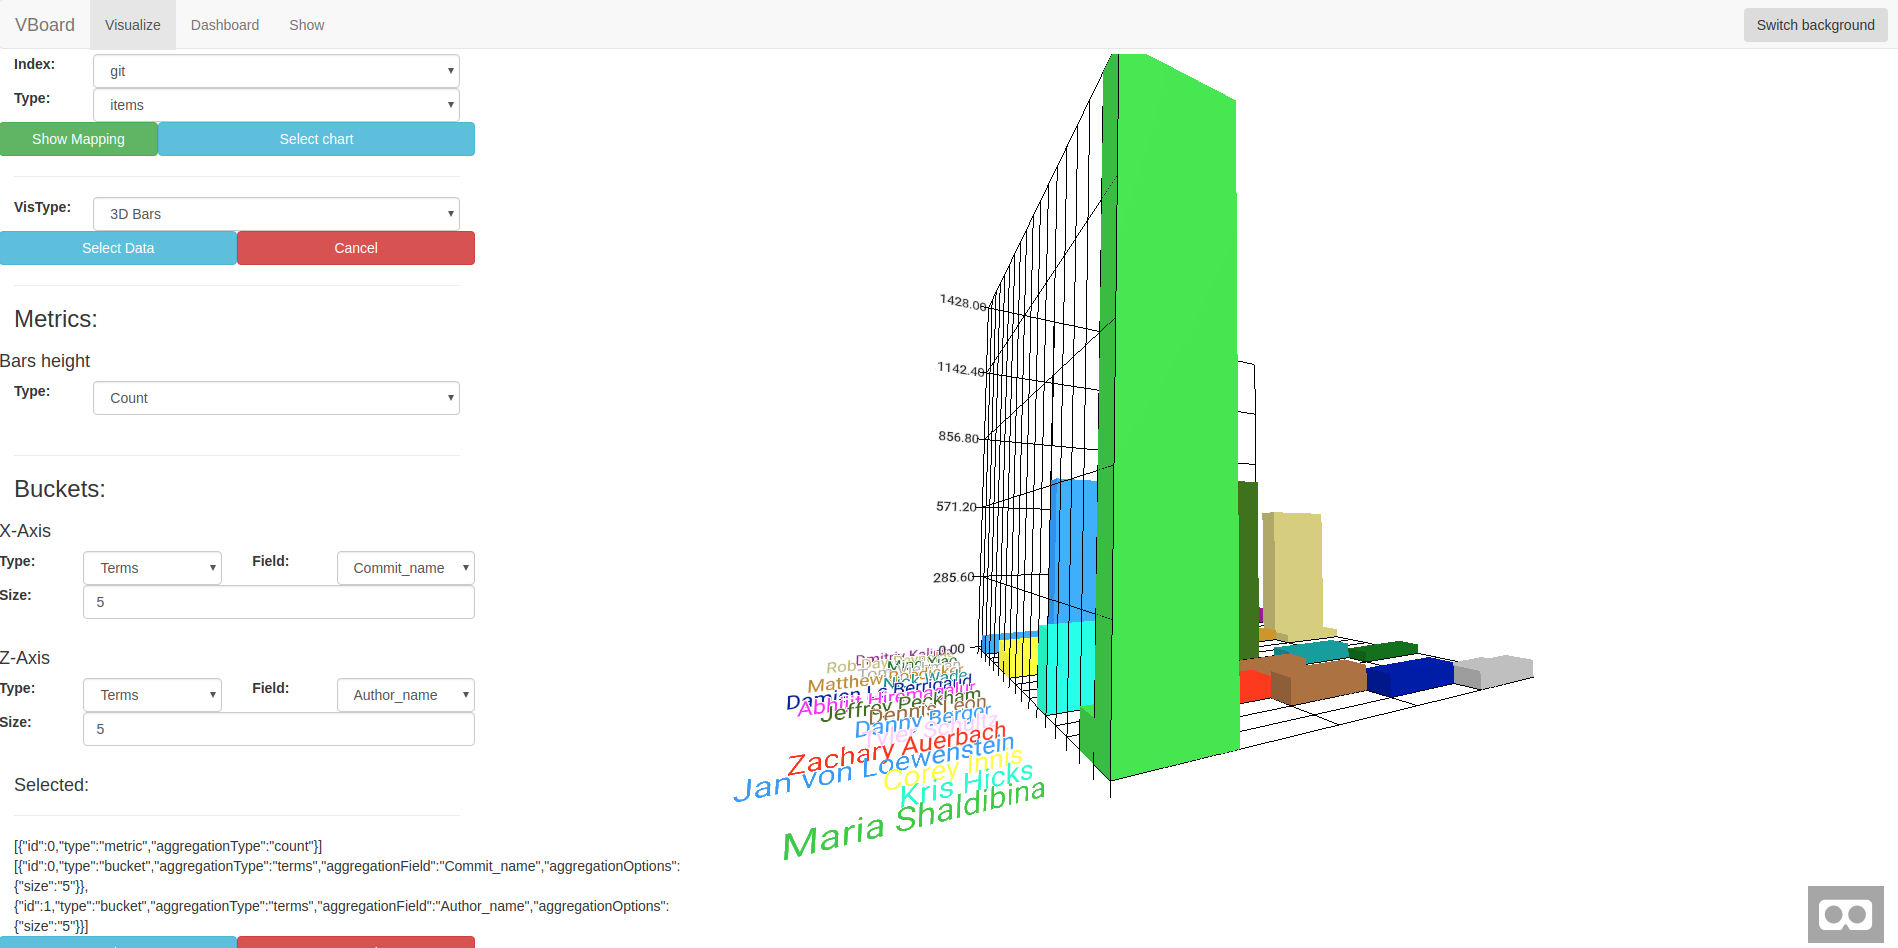
\includegraphics[width=16cm, keepaspectratio]{img/development/examplevisaframedc}
  \caption{Visualization example with A-FrameDC}
  \label{fig:examplestandalone}
\end{figure}

\begin{figure}[H]
  \centering
  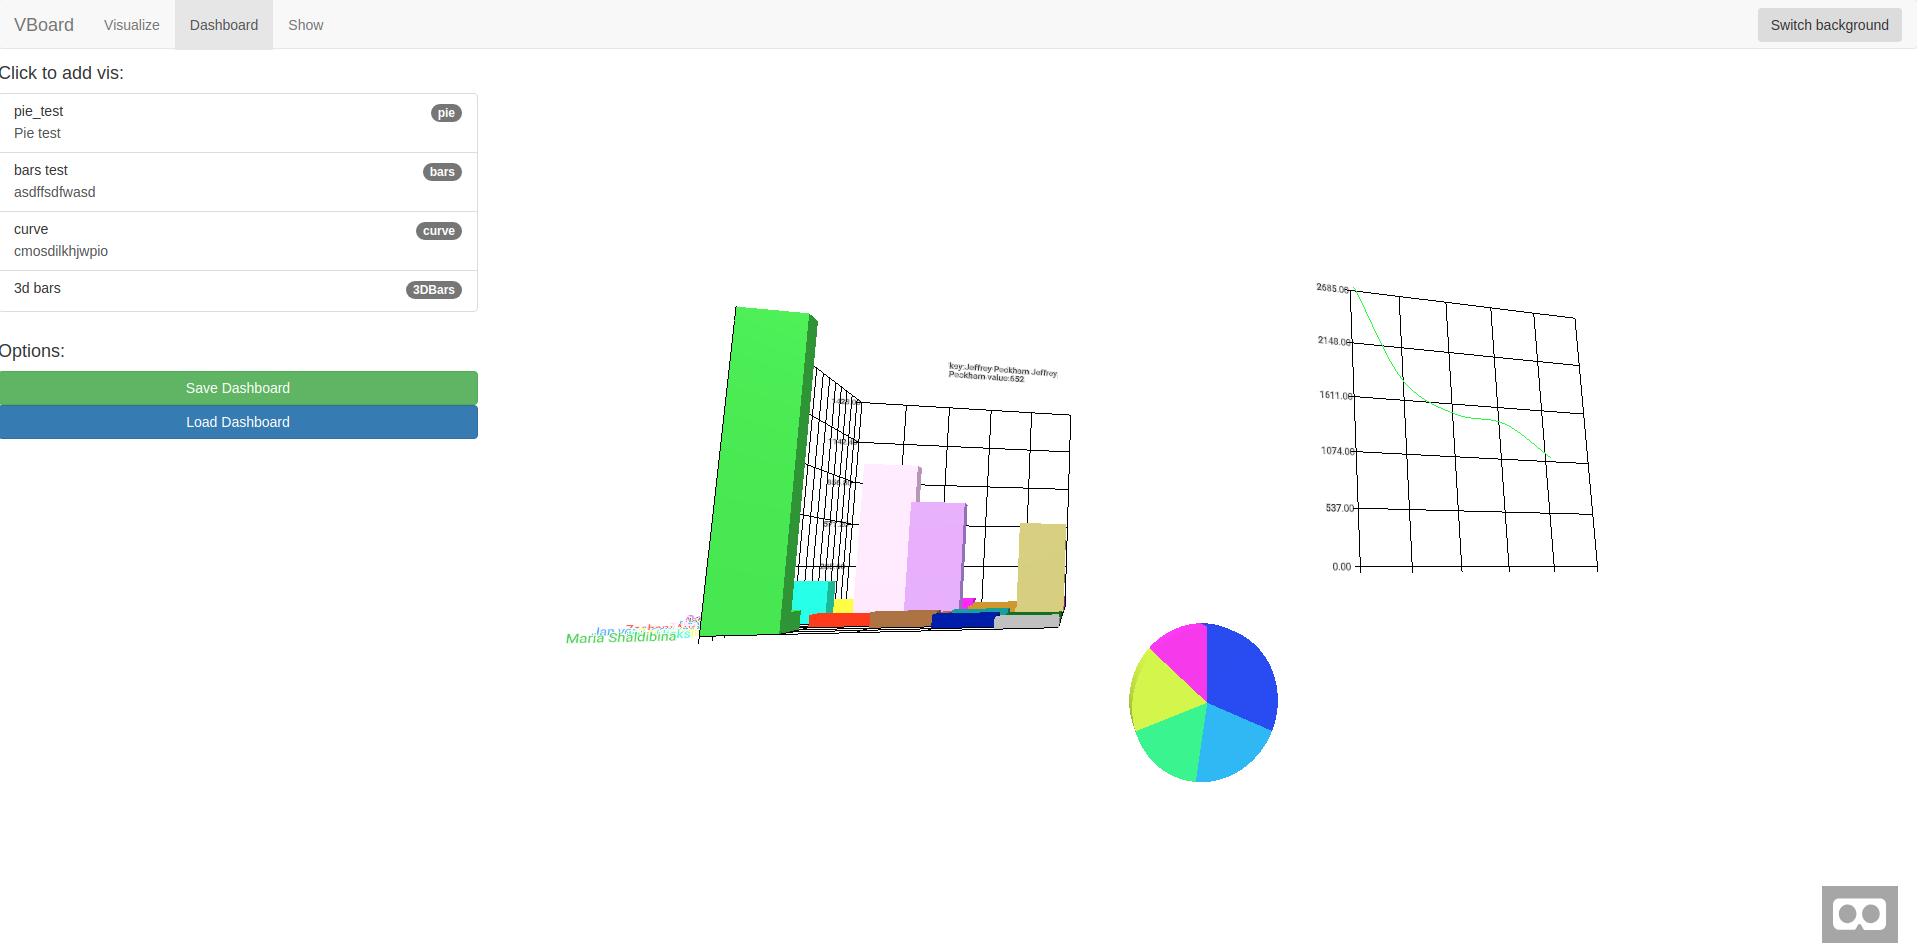
\includegraphics[width=16cm, keepaspectratio]{img/development/dashtestaframedc}
  \caption{Dashboard example with A-FrameDC}
  \label{fig:examplestandalone}
\end{figure}



\section{Iteration 7: Customization and optimization}

Con el fin de realizar una aplicación limpia y facil de usar, se han desarrollado varias customizaciones para mejorarla, así como una optimización del código para que sea rápido y escalable:

\begin{enumerate}
    \item Change background functionality
    \item Init process VBoard
    \item Rotation of the charts
    \item Information/Error messages when querying ElasticSearch
\end{enumerate}

\subsection{Change background functionality}

Para poder ver los dashboards en VR y en el modo "stand alone", implementamos un algoritmo que cambia entre unos fondos de pantalla que se encuentran en la aplicación, añadiendo un botón en la barra de navegación para irlo cambiando. Estos fondos son limitados y se encuentran en el código de la aplicación:

\begin{figure}[H]
  \centering
  
\includegraphics[width=6cm, keepaspectratio]{img/development/switchbackgroundbutton}
  \caption{Switch background button in the navbar}
  \label{fig:examplestandalone}
\end{figure}


Una vez guardado el dashboard, el fondo que tiene asignado se guardará con él, así cuando se cargue se cargará con él, lo mismo pasa cuando se carga el modo stand alone y VR:

\begin{figure}[H]
 \centering
  \subfloat[In Dashboard tab]{
    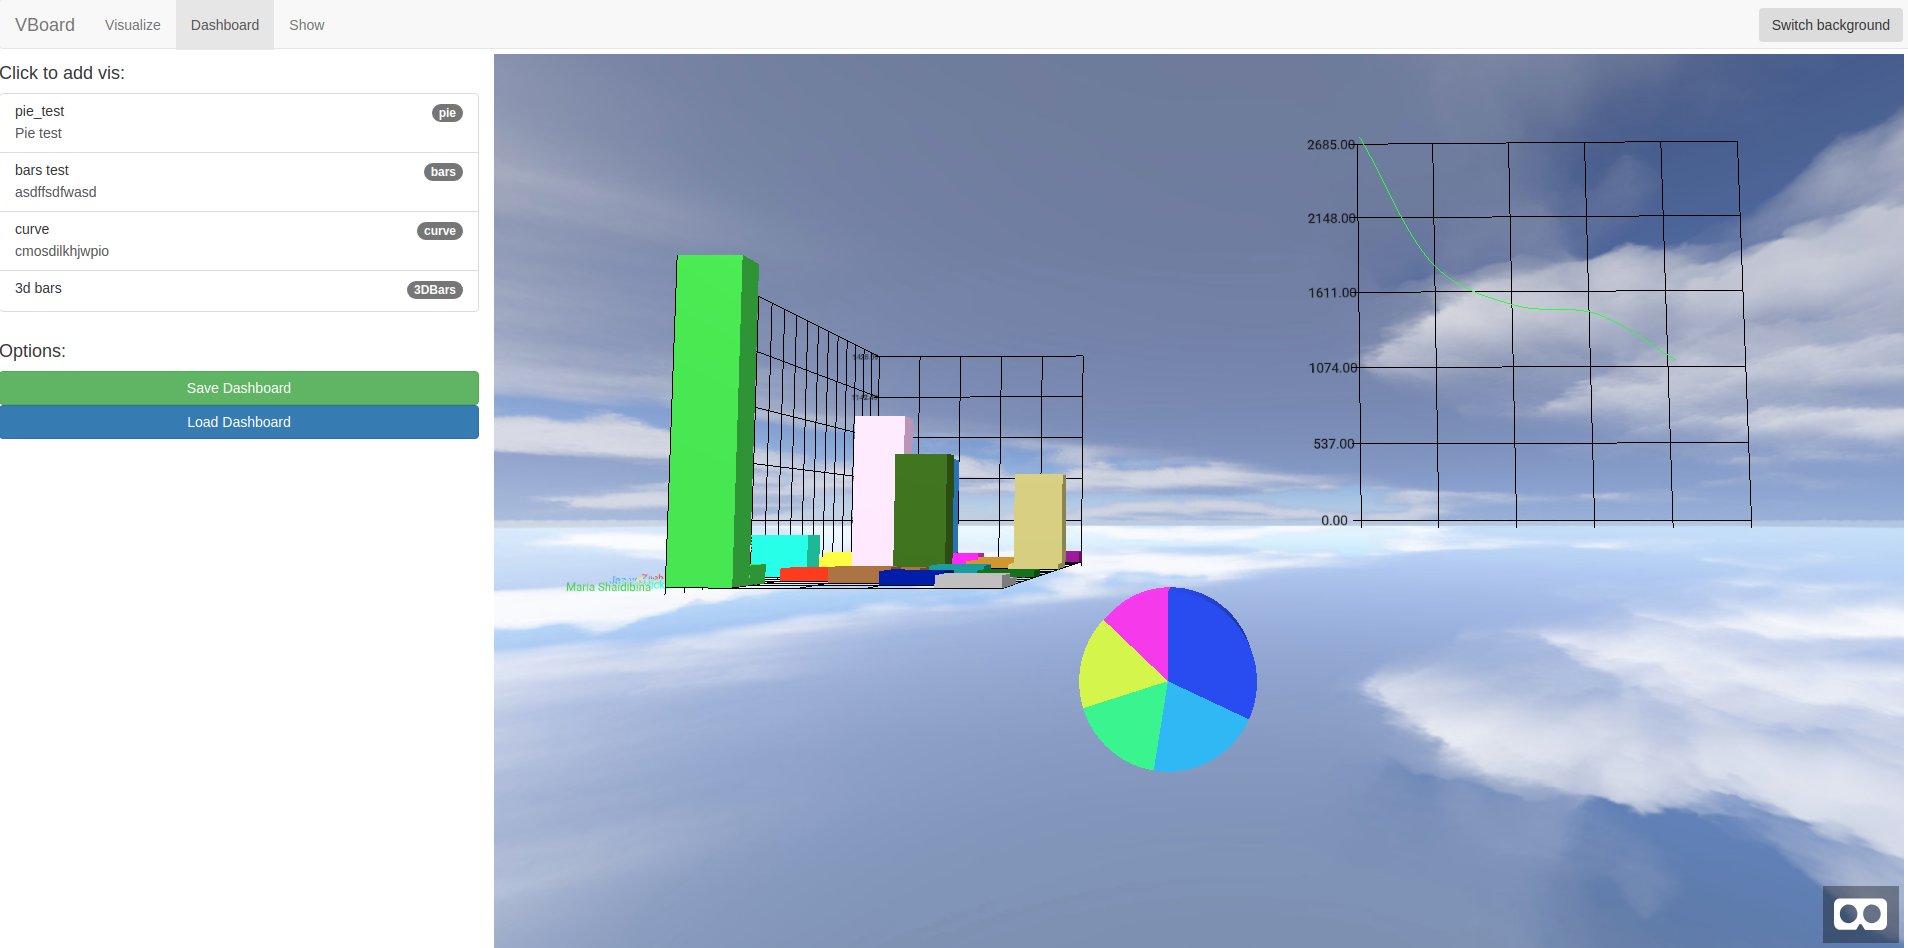
\includegraphics[width=0.5\textwidth]{img/development/backgroundaframedc}}
  \subfloat[In Show tab]{
    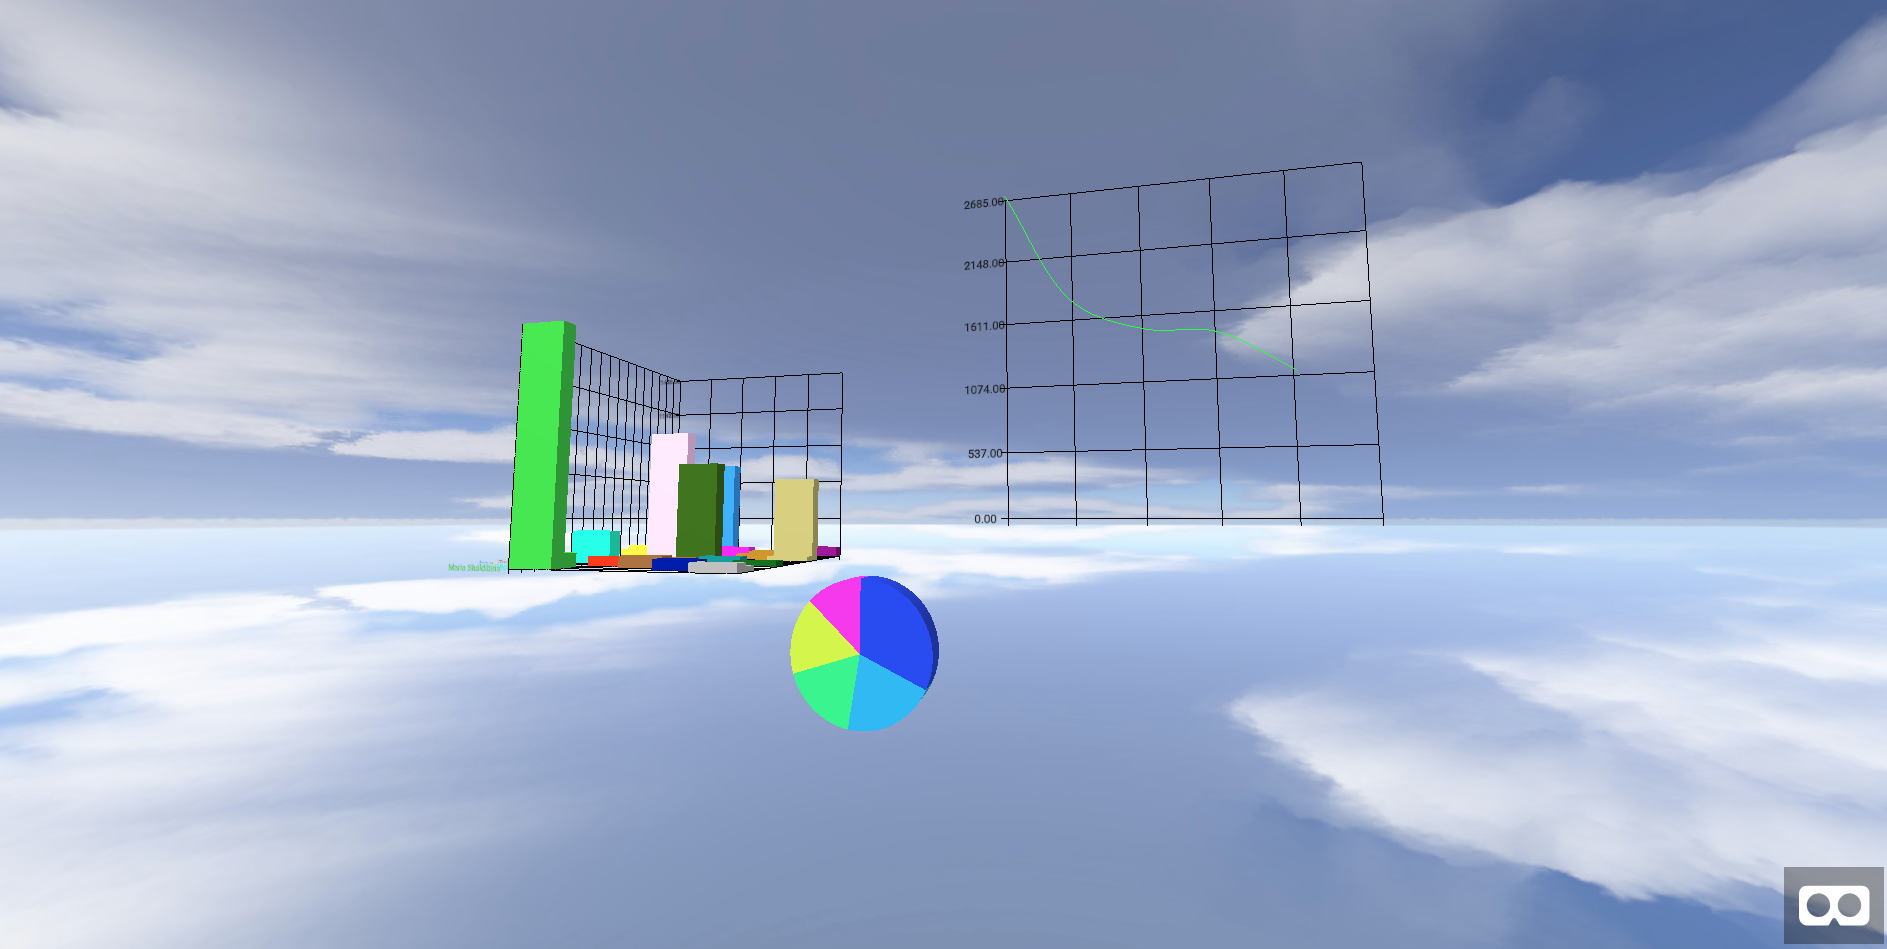
\includegraphics[width=0.5\textwidth]{img/development/showbackgroundaframedc}}
 \caption{Dashboard with background}
 \label{f:threedcexamples}
\end{figure}


Esta funcionalidad también ha sido integrada en ThreeDC.



\subsection{Init process VBoard}

Para poder crear el índice (index) de VBoard en ElasticSearch y comprobar que la aplicación se ha conectado bien y tiene acceso al índice, hemos desarrollado una nueva fase a la aplicación, la fase llamada Init, con su propio controlador AngularJS.

Esta fase comprueba que tiene acceso al ElasticSearch definido en el servicio de Angular dentro de la aplicación. Si la conexión es correcta intentará acceder al índice ".vboard", si no lo encuentra, trata de crearlo, haciendo una petición PUT con el mapping. Si no es correcta aparecerá un mensaje de error en la pantalla:

\begin{figure}[H]
  \centering
  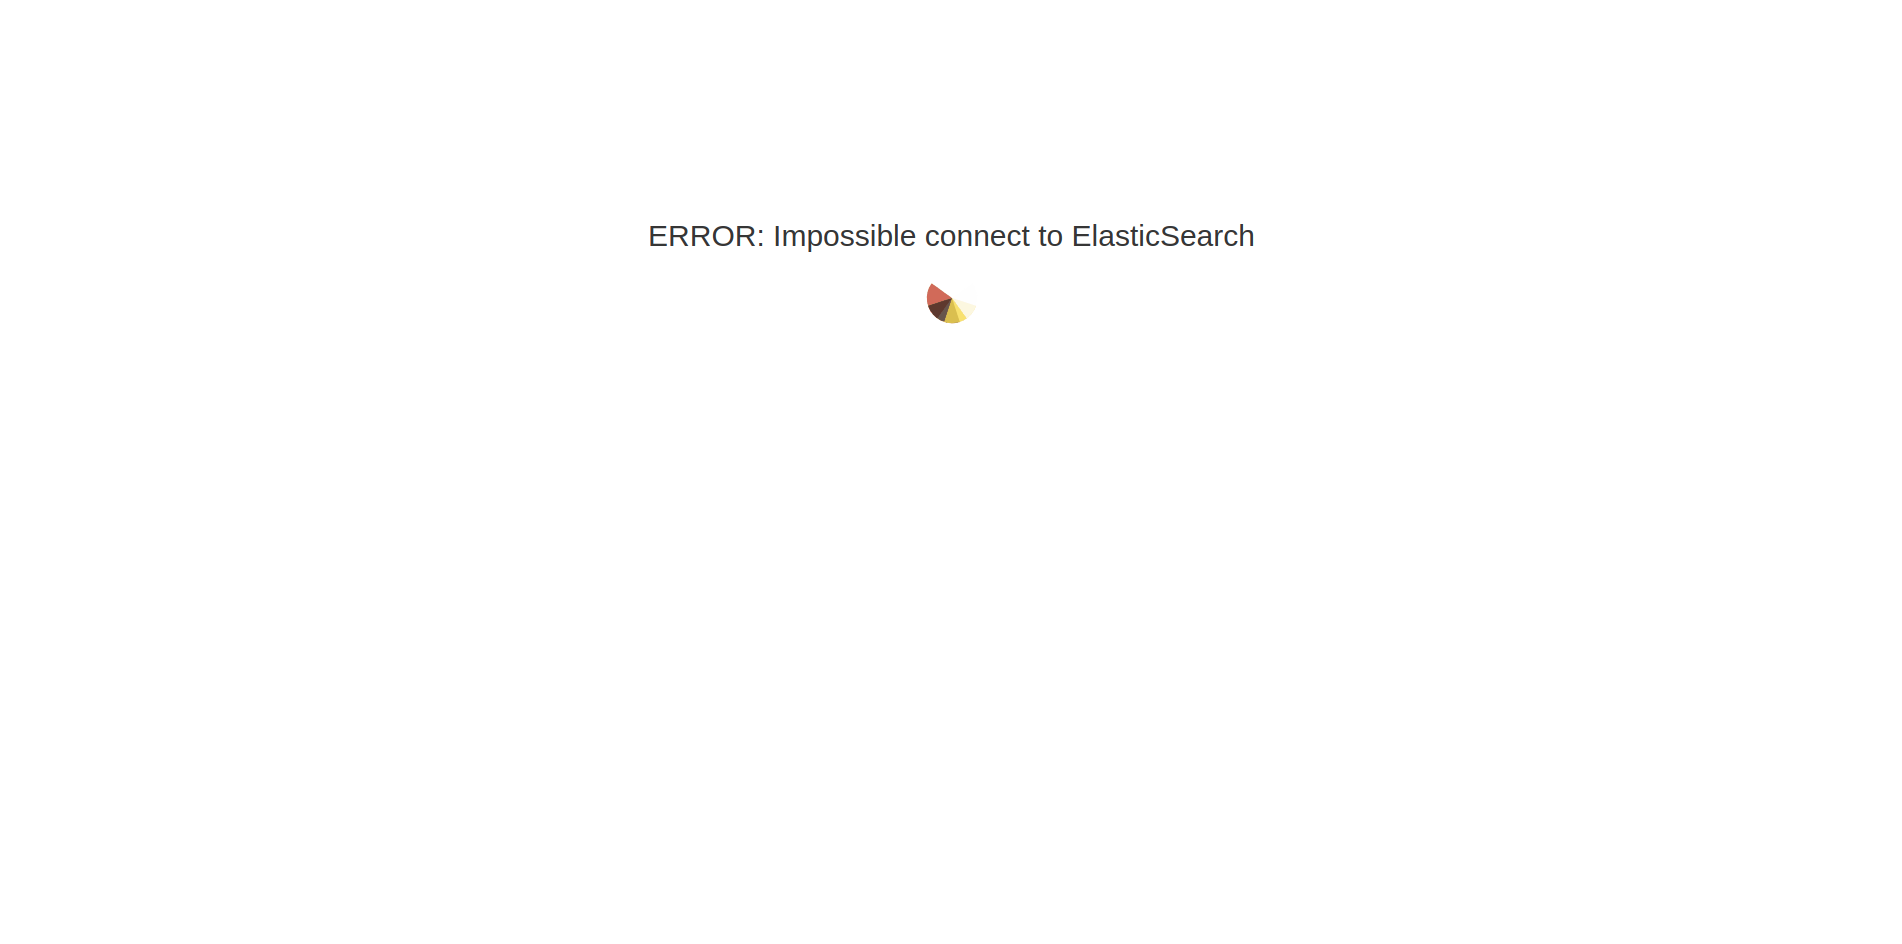
\includegraphics[width=16cm, keepaspectratio]{img/development/errorconnectes}
  \caption{Switch background button in the navbar}
  \label{fig:examplestandalone}
\end{figure}

En el caso de que se haya podido conectar y tener acceso al índice ".vboard" aparecerá un mensaje diciendo que todo ha ido bien redirigiendo al usuario a la pestaña Visualize:

\begin{figure}[H]
  \centering
  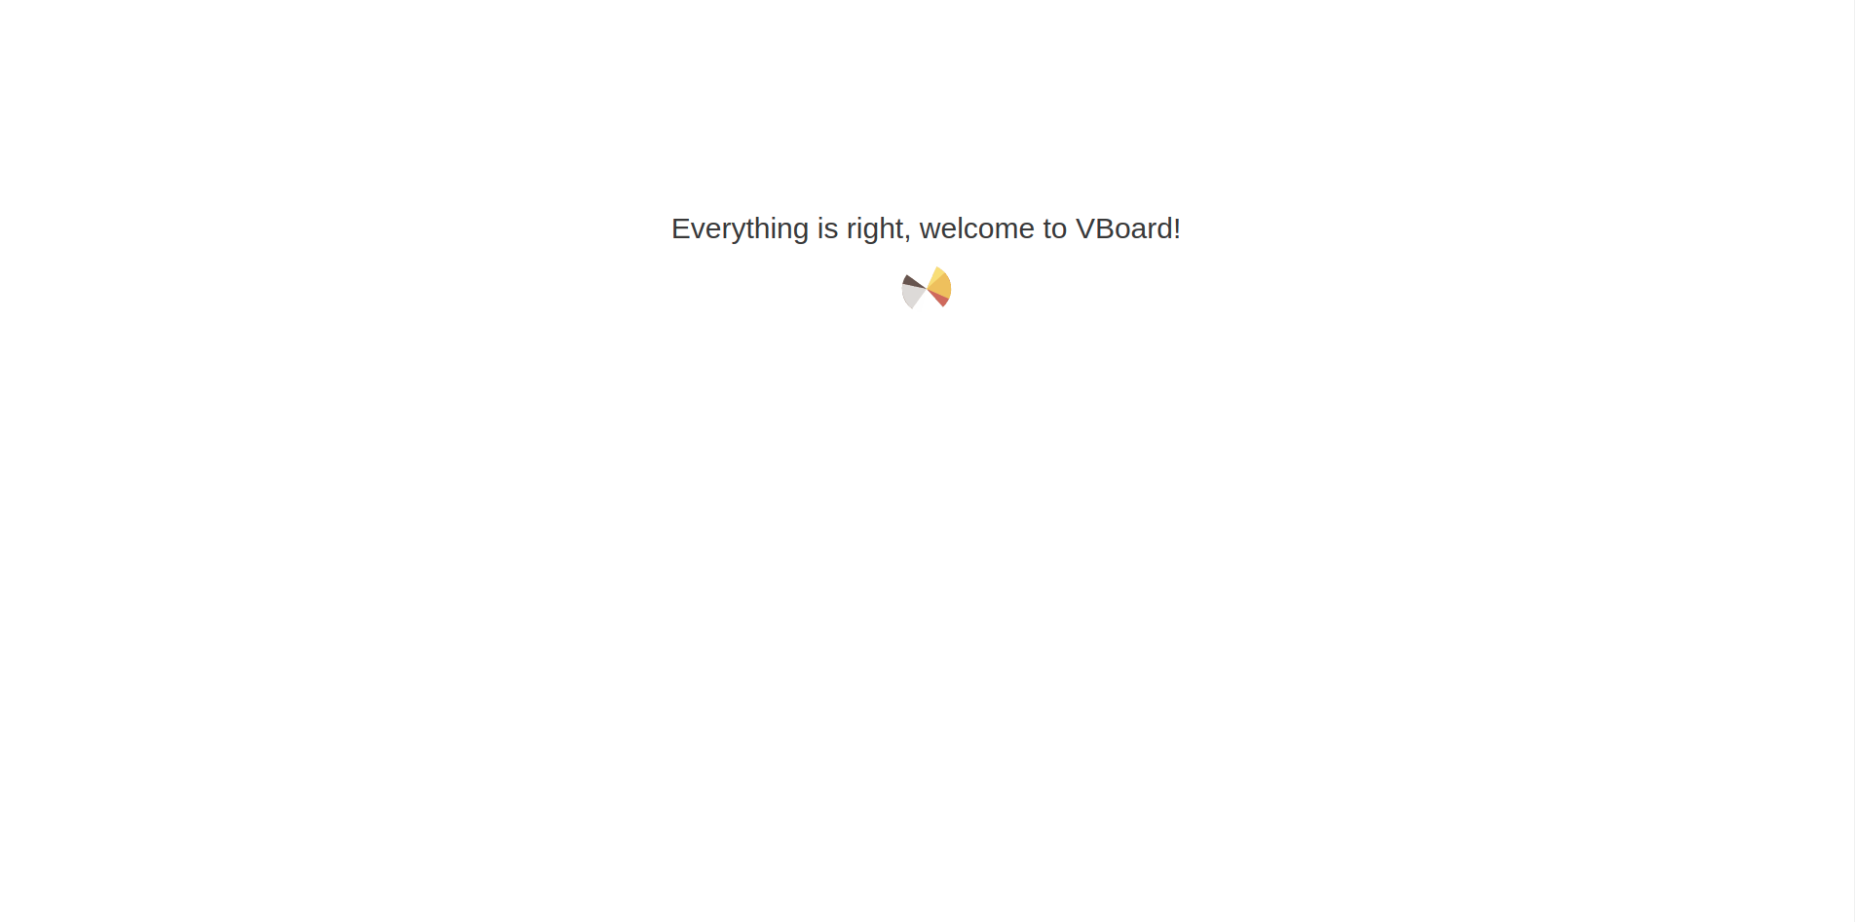
\includegraphics[width=16cm, keepaspectratio]{img/development/msgright}
  \caption{Switch background button in the navbar}
  \label{fig:examplestandalone}
\end{figure}

Para toda esta funcionalidad se han añadido más métodos a la librería genES para todas estas peticiones. Siempre se comprueba que la conexión con ElasticSearch está activa, si no se redirigirá a la pantalla de error mostrada anteriormente

\subsection{Rotation of the charts}

No tiene sentido tener un dashboard en 3D y VR y que no se puedan colocar las visualizaciones con una rotación dada. Lamentablemente, ThreeDC y A-frameDC no admiten está opción en su método de construcción de visualizaciones, por lo que hemos decidido que ibámos a desarrollar nosotros mismo esa funcionalidad modificando directamente la API de A-frameDC.

La modificación es sencilla ya que aun que los métodos de la API, lo no permitan, existe esa funcionalidad por debajo, directamente en A-Frame. Por lo tanto una vez modificados esos métodos solamente hay que añadir en el modal de añadir visualizaciones a un dashboard, 3 nuevos inputs para definir la rotación en 3 ejes, "x", "y" y "z" (ya que estamos en un entorno en 3D):

\begin{figure}[H]
  \centering
  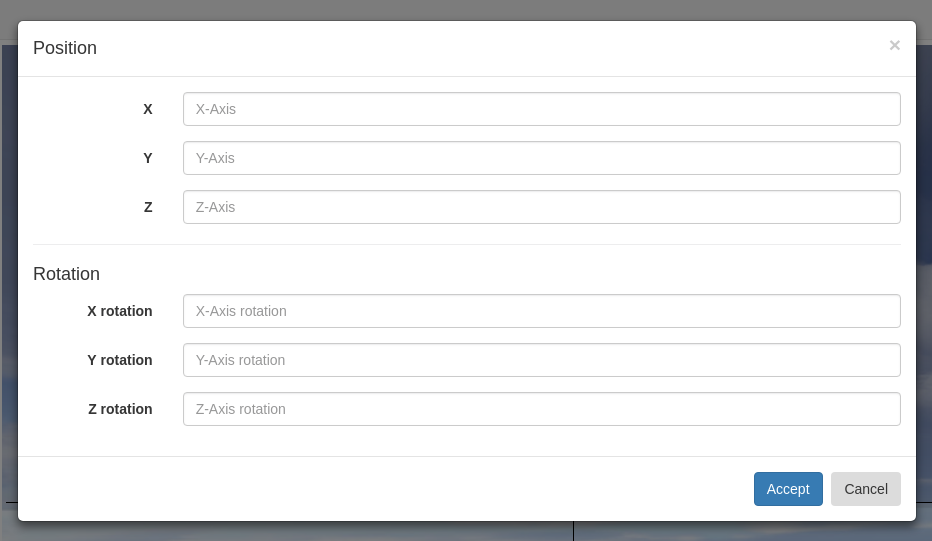
\includegraphics[width=16cm, keepaspectratio]{img/development/newformaframedc}
  \caption{Form now with rotation section}
  \label{fig:examplestandalone}
\end{figure}

Con esta funcionalidad ya podemos poner visualizaciones en la escena en un abanico de 360 grados.

\subsection{Information/Error messages when querying ElasticSearch}

Otra mejora importante para la aplicación es notificar al usuario cuando accede a ElasticSearch para comprobar que ha la acción ha sido correcta o errónea. Para ello hemos incluido la bilbioteca "angular-ui-notification" para mostrar metiante pequeños modals en la esquina superior derecha, mensajes de error o de success.

Así, si el usuario no ha podido acceder a ElasticSearch para guardar/cargar un elemento, se mostraŕa un cuadro de notificación de error, y en cambio, si se ha podido acceder correctamente, se mostrará un cuadro de notificación verde para mostrar que ha ido correctamente. Las siguientes capturas muestran unos ejemplos de el uso de estos cuadros de información:

\begin{figure}[H]
 \centering
  \subfloat[Error notification]{
    
\includegraphics[width=0.5\textwidth]{img/development/error_noti}}
  \subfloat[Success notification]{
    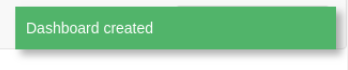
\includegraphics[width=0.5\textwidth]{img/development/success_noti}}
 \caption{Notifications}
 \label{f:threedcexamples}
\end{figure}


Entendemos que hay mucho trabajo por delante y que quedan muchas mejoras, las cuales serán comentadas en el último capítulo de la memoria donde se detalla el trabajo futuro sobre esta aplicación.

\section{Iteration 8: Dockerize application}
\label{sec:dockerize}

La última iteracción, de gran importancia, ha sido dockerizar la aplicación para que se pueda desplegar como un contenedor docker de manera fácil y escabale, de esta manera, cualquier persona con conocimentos básicos de Docker puede desplegar VBoard de manera sencilla sin tener que seguir muchos pasos de instalación tediosos.

Para ello, se han creado 2 imágenes de docker para VBoard, una de ellas con el motor de renderizado ThreeDC y otra con A-FrameDC, siendo la de A-FrameDC su principal imagen. Lo primero es generar un Dockerfile definiendo el servicio de la apliación. En este caso se ha partido de una imagen "node-8" ya que utilizamos el servidor http de node como servidor para desplegar VBoard. El archivo Dockerfile es bastante sencillo ya que lo único que hace es clonarse el repo sobre una branch determinada (para diferenciar la version ThreeDC y A-FrameDC), instalar las dependencias npm (entre ellas también el servidor http), exponer el puerto 8080 y definir como "entrypoint" un script escrito en shell que configura la conexión con ElasticSearch e inicia el servidor:

\begin{lstlisting}[frame=single]
FROM node:8.12

MAINTAINER David Moreno Lumbreras "dmorenolumb@gmail.com"

RUN apt-get update -y

# Clone the repository
RUN git clone https://github.com/dlumbrer/VBoard -b integration-aframedc

# Install dependencies
WORKDIR VBoard
RUN npm install

# Install http-server
RUN npm install -g http-server

# Copy entrypoint
COPY docker-entrypoint.sh .
RUN chmod 755 docker-entrypoint.sh

# Expose port ant init application
EXPOSE 8080
CMD ["./docker-entrypoint.sh"]
\end{lstlisting}

El docker-entrypoint está diseñado para que se pueda definir como variable de entorno la IP del ElasticSearch al que se quiera conectar VBoard (\textit{\$ELASTICSEARCH\_URL}), y si no se ha definido esta variable, que automáticamente se conecte al ElasticSearch del host del contenedor:

\begin{lstlisting}[frame=single]
#!/bin/bash

set -e

if [ "$ELASTICSEARCH_URL" != "" ]; then
        # If defined in the docker-compose
        sed -e "s|host: 'http://localhost:9200',$|host: '$ELASTICSEARCH_URL',|" -i /VBoard/app/service/ESService.js
else
        IP_HOST=$(/sbin/ip route|awk '/default/ { print $3 }')
        sed -e "s|host: 'http://localhost:9200',$|host: 'http://$IP_HOST:9200',|" -i /VBoard/app/service/ESService.js
fi

http-server
\end{lstlisting}

Una vez definidas estas imágenes y testeadas, el siguiente paso es alojarlas en docker-hub, el lugar donde se almacenan imágenes de docker para que cualquier persona pueda acceder a ellas mediante un tag. Para ello, se hace un link con el repositorio donde se encuentra el Dockerfile y se definen tags de imágenes que serán construidas a partir de una rama o tag del repositorio.

En el caso de VBoard, los Dockerfile de la version de ThreeDC y A-FrameDC se encuentran en la rama "docker", por lo que configuramos la construcción de imágenes de la siguiente manera:

\begin{figure}[H]
  \centering
  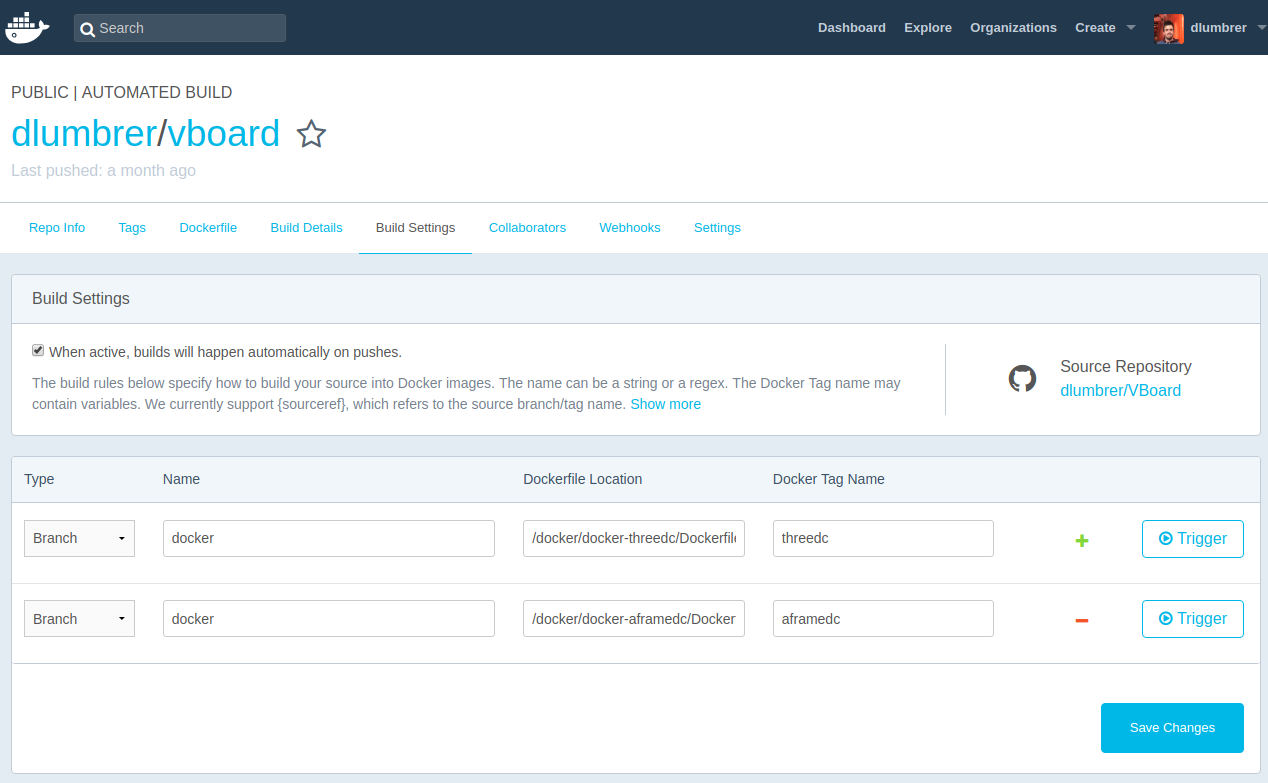
\includegraphics[width=16cm, keepaspectratio]{img/development/docker-hub-0}
  \caption{Build Settings for VBoard}
  \label{fig:examplestandalone}
\end{figure}

Así tendremos dos imágenes de VBoard disponibles, cada una con un tag distinto:

\begin{figure}[H]
  \centering
  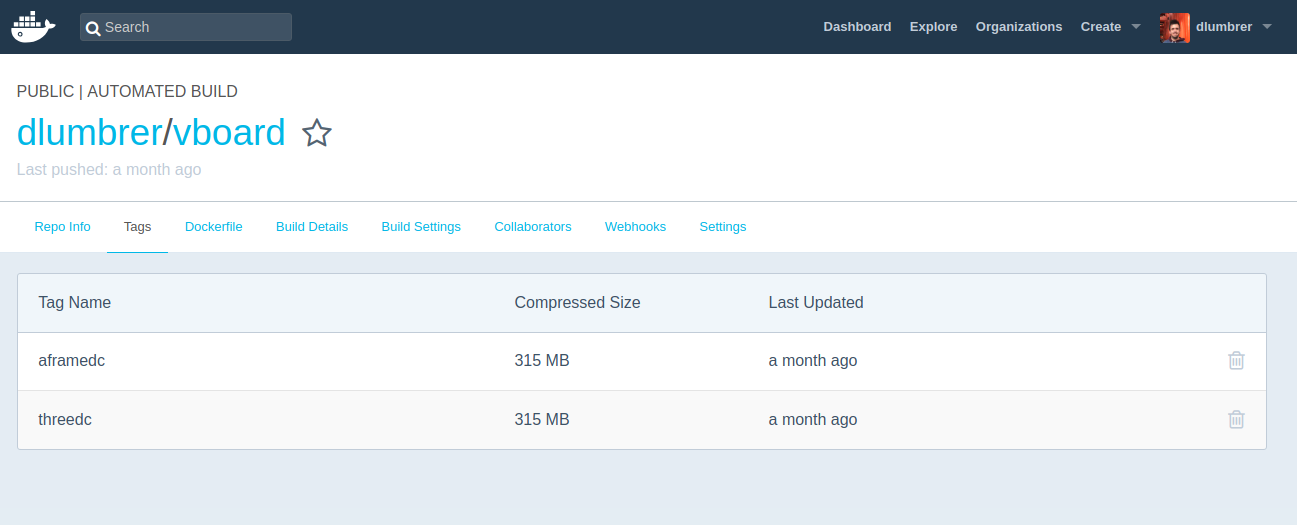
\includegraphics[width=16cm, keepaspectratio]{img/development/dockerhub}
  \caption{Image tags for VBoard}
  \label{fig:examplestandalone}
\end{figure}

Con las imágenes construidas, podremos descargarlas y lanzar contenedores de ellas simplemente desplegando los tags \textit{dlumbrer/VBoard:aframedc} y \textit{dlumbrer/VBoard:threedc}.

 
%%%%%%%%%%%%%%%%%%%%%%%%%%%%%%%%%%%%%%%%%%%%%%%%%%%%%%%%%%%%%%%%%%%%%%%%%%%%%%%%
%%%%%%%%%%%%%%%%%%%%%%%%%%%%%%%%%%%%%%%%%%%%%%%%%%%%%%%%%%%%%%%%%%%%%%%%%%%%%%%%
% RESULTADOS %
%%%%%%%%%%%%%%%%%%%%%%%%%%%%%%%%%%%%%%%%%%%%%%%%%%%%%%%%%%%%%%%%%%%%%%%%%%%%%%%%
\cleardoublepage
\chapter{Design and results}
\label{chap:dai}

\section{Introduction}
\label{sec:dint}

In this chapter we will describe the aspects of the final application. We will start defining its structure, in code and in visualization. Then, we will explain its functioning next to a user's guide in order to define de different types of visualization and dashboard that the application has. Finally, we will test the application with data offered by the product owner.

\section{Structure}

Como explicamos en la sección \ref{sec:it1}, para desarrollar una aplicación front-end en AngularJS, se ha seguido una estructura de archivos estándar de este framework. Siguiendo el modelo ya presentado, VBoard tiene la siguiente estructura de archivos:

\begin{figure}[H]
  \centering
  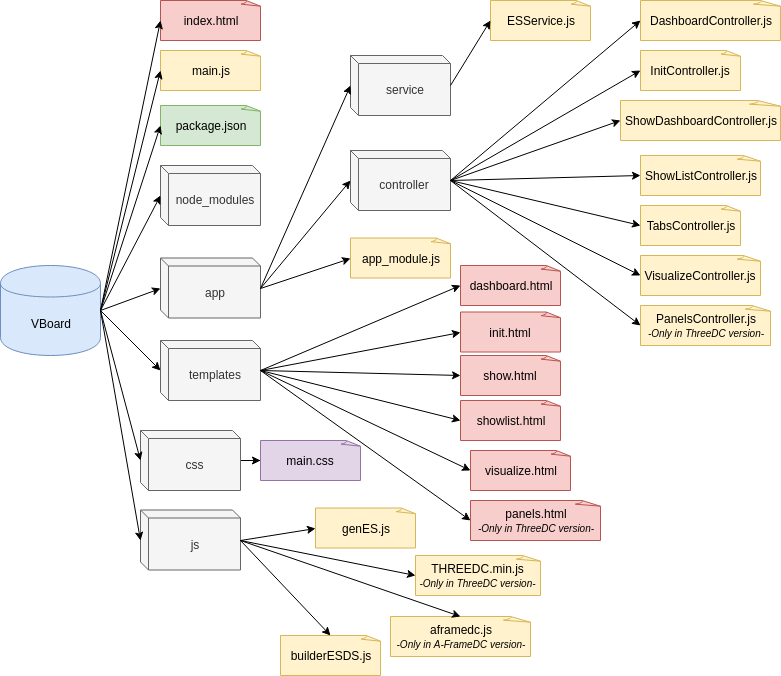
\includegraphics[width=16cm, keepaspectratio]{TFM/img/results/Vboard.png}
  \caption{Diagram of the files}
  \label{fig:codediagram}
\end{figure}

Los archivos de color amarillo corresponden a códigos JavaScript, los de color rojo a códigos HTML, los morados a código CSS y los verdes a archivos JSON.

Concretamente:
\begin{itemize}
    \item Archivo \textit{index.html}: Archivo html básico donde se cargan las bibliotecas externas (CDN or in local) y donde está definida la barra de navegación de VBoard.
    \item Archivo \textit{main.js}: Archivo donde se define la aplicación AngularJS, en este caso VBoard.
    \item Achivo \textit{package.json}: Archivo donde se encuentra el metadata de VBoard así como las dependencias necesarias npm para su posterior instalación.
    \item Carpeta \textit{node\_modules}: Lugar donde las dependencias npm serán instaladas.
    \item Carpeta \textit{app}: Dentro de esta carpeta se encuentra el "core" de la apliación JavaScript, dentro están las siguientes carpetas:
    \begin{itemize}
        \item Carpeta \textit{service}: Carpeta donde se encuentran los servicios de AngularJS que se van a usar en VBoard, en este caso solo hay uno, con el nombre de \textit{ESService.js} donde se define el cliente ElasticSearch que se va a usar en VBoard.
        \item Carpeta \textit{controller}: Dentro de esta carpeta están todos los controladores de las diversas zonas de VBoard, se encuentra el controlador de toda la lógica de la barra de navegación en el archivo \textit{TabsController.js}, la lógica del proceso de inicio de VBoard en el archivo \textit{InitController.js}, la lógica de cada uno de los tabs disponibles "Visualize, Panels, Dashboard and Show" es sus archivos correspondientes.
        \item Achivo \textit{app\_module.js}: Archivo donde se instancia la apliación VBoard, donde se definen todos los controladores, templates y archivos del framework AngularJS que necesita.
    \end{itemize}
    \item Carpeta \textit{templates}: Dentro de esta carpeta están los 5 códigos html correspondientes a las 5 zonas que requieren HTML que hay dentro de VBoard, Init, Visualize, Panels, Dashboard y Show.
    \item Carpeta \textit{css}: En esta carpeta se encuentran los códigos CSS, en este caso solo hay uno ya que el CSS utilizado es mínimo y por lo tanto es un gran punto a mejorar en VBoard.
    \item Carpeta \textit{js}: En esta carpeta se encuentran las bibliotecas JavaScript que no se han instalado por npm, es decir, en este caso genES y builderESDS que han sido desarrolladas por nosotros, y las bibliotecas de renderización 3D, \textit{aframedc.js} y \textit{THREEDC.min.js}. 
\end{itemize}

La estructura visual está definida también en la sección \ref{sec:it1}, por lo que no se detallará otra vez, en las siguientes secciones se explicará una guía de usuario y unos ejemplos donde todo quedará claro. 


\section{Installation steps}
There are few ways to install VBoard, from the source code in the repository, from the releases, or from the docker image that is in dockerhub. All these installation steps are included in the README.md\footnote{\url{https://github.com/dlumbrer/VBoard}} of the repository.

\subsection{From repository}
Directly installation from the source code, the steps are:
\begin{enumerate}
    \item Clone the repository, choosing a different branch in order to change between ThreeDC and A-FrameDC
    \begin{itemize}
        \item For A-FrameDC version: \textit{git clone https://github.com/dlumbrer/VBoard-UI -b integration-aframedc}
        \item For ThreeDC version: \textit{git clone https://github.com/dlumbrer/VBoard-UI -b integration-threedc}
    \end{itemize}
    \item Change directory: \textit{cd VBoard}
    \item Install npm dependencies, it is necessary to have installed node: \textit{npm install}
    \item (Optional) Install node http-server: \textit{npm install -g http-server}
    \item Run VBoard server: \textit{http-server}
\end{enumerate}

The fifth step is optional because you can use any server of http, for instance the http simple server from python.

\subsection{From releases}
This is the easiest way to launch VBoard if don't want to install it via source code or docker. It is so simple that you have to download the zip/tar binarie of the selected version (ThreeDC or A-FrameDC) from the GitHub VBoard releases page \footnote{\url{https://github.com/dlumbrer/VBoard/releases}}, go inside the uncompressed folder and launch it with your favourite http-server (I recommend the http-server from node).

\subsection{Docker}
As we explained in section \ref{sec:dockerize}, there are docker images of the two versions of VBoard. The information about the images are inside the "docker" branch of the repository\footnote{\url{https://github.com/dlumbrer/VBoard/tree/docker}}, also, there are inside a few examples of how to deploy VBoard using docker-compose.

If we want to deploy VBoard, we can do it easily with docker launching a container in one line, but the easiest and useful way is to use docker-compose. There are two ways to deploy VBoard with docker-compose, one with ElasticSearch included or one just with VBoard:

\begin{itemize}
    \item \textbf{A-FrameDC or ThreeDC + ElasticSearch}: If you want a full installation with the A-FrameDC or ThreeDC version and a ElasticSearch, I recommend to use this docker-compose:
    \begin{lstlisting}[frame=single]
    elasticsearch:
      image: docker.elastic.co/elasticsearch/elasticsearch:5.6.0
      ports:
        - "9200:9200"
      volumes:
        - ./config/elasticsearch.yml:/usr/share/elasticsearch/config/elasticsearch.yml:ro
      environment:
        - ES_JAVA_OPTS=-Xms2g -Xmx2g
        - transport.host=127.0.0.1
        - xpack.security.enabled=false
    
    vboard:
      image: dlumbrer/vboard:aframedc
      # image: dlumbrer/vboard:threedc # Uncomment this line if you want the ThreeDC version
      ports:
        - "8080:8080"
    \end{lstlisting}
    Note that the VBoard app will be connected to ElasticSearch automatically.
    
    \item \textbf{A-FrameDC or ThreeDC without ElasticSearch}: This compose will deploy just VBoard:
    \begin{lstlisting}[frame=single]
    vboard:
      image: dlumbrer/vboard:aframedc
      # image: dlumbrer/vboard:threedc # Uncomment this line if you want the ThreeDC version
      ports:
        - "8080:8080"
      environment:
        - ELASTICSEARCH_URL=http://localhost:9200
    \end{lstlisting}
    \textbf{Important}: You have to modify the environment variable "ELASTICSEARCH\_URL" to you ElasticSearch url.
    
    \item Moreover, we offer a docker-compose file in order to deploy just ElasticSearch, for instance if you want an ElasticSearch in one machine and VBoard in other, or you want to install VBoard from releases or source code but you want to use ElasticSearch in a docker container:
    \begin{lstlisting}[frame=single]
    elasticsearch:
      image: docker.elastic.co/elasticsearch/elasticsearch:5.6.0
      ports:
        - "9200:9200"
      volumes:
        - ./config/elasticsearch.yml:/usr/share/elasticsearch/config/elasticsearch.yml:ro
      environment:
        - ES_JAVA_OPTS=-Xms2g -Xmx2g
        - transport.host=127.0.0.1
        - xpack.security.enabled=false
    \end{lstlisting}
    
In order to deploy VBoard with docker, it is needed a few acknowledge of Docker.




\end{itemize}

\section{User Guide}

Later, we will define a user guide, explaining step by step how to init VBoard, how to produce visualizations, how to save it, how to produce dashboards and how to save it and see it in the stand-alone version.  As the menu and the process is the same, we will explain the user guide for the A-FrameDC version, focusing in examples and how to take advantage of all functionality of VBoard. So we explain how to produce an entire dashboard with visualizations from scratch:

\subsection{Init VBoard}

Antes de todo, VBoard hará una comprobación de su conexión a ElasticSearch, estos son los pasos que se verán al entrar en la aplicación:

\begin{enumerate}

    \item Primero, VBoard notificará al usuario que está realizando configuraciones:
    \begin{figure}[H]
      \centering
      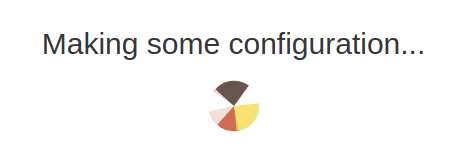
\includegraphics[width=8cm, keepaspectratio]{img/results/Init1}
      \caption{First info message from VBoard}
      \label{fig:onlynodes}
    \end{figure}
    En el caso de que no pueda conectarse a ElasticSearch se mostrará este mensaje de error:
    \begin{figure}[H]
      \centering
      
\includegraphics[width=11cm, keepaspectratio]{img/results/Init2}
      \caption{Error connecting to ElasticSearch}
      \label{fig:onlynodes}
    \end{figure}
    \item Una vez conectado a ElasticSearch, buscará el índice \textit{.vboard}, y pueden suceder dos cosas:
    \begin{itemize}
        \item Que el índice no exista, por lo que tratará de crearlo mostrando este mensaje de información:
        \begin{figure}[H]
          \centering
          \includegraphics[width=9cm, keepaspectratio]{img/results/Init3}
          \caption{Creating .vboard index}
          \label{fig:onlynodes}
        \end{figure}
        Para ello, subirá el mapping del índice, en el caso de que no haya podido subir el mapping por alguna razón, se mostrará el siguiente mensaje de error:
        \begin{figure}[H]
          \centering
          \includegraphics[width=9cm, keepaspectratio]{img/results/Init4}
          \caption{Unexpected error}
          \label{fig:onlynodes}
        \end{figure}
        Si ha subido bien el mapping, se notificará de que todo está bien y se entrará en VBoard:
        \begin{figure}[H]
          \centering
          \includegraphics[width=11cm, keepaspectratio]{img/results/Init5}
          \caption{Index and mapping created}
          \label{fig:onlynodes}
        \end{figure}
        \item Que el índice ya esté creado y por lo tanto todo está listo, se mostrará el siguiente mensaje de información:
        \begin{figure}[H]
          \centering
          \includegraphics[width=9cm, keepaspectratio]{img/results/Init6}
          \caption{Everything right}
          \label{fig:onlynodes}
        \end{figure}
    \end{itemize}
\end{enumerate}

Finalmente, si todo ha cargado bien, VBoard te redirigirá a la pestaña Visualize.

\subsection{Visualize}

In order to build a 3D visualization, go to the tab "Visualize" and follow these steps:
\begin{enumerate}
    \item Select the index and the type of your ElasticSearch where the data is going to be visualized, then click on "Select chart" button:
    \begin{figure}[H]
      \centering
      \includegraphics[width=8cm, keepaspectratio]{img/results/selectindex}
      \caption{Index and type selection}
      \label{fig:onlynodes}
    \end{figure}
    Note that there are another button call "Show mapping", it is explained at the end of this section, in the Options section.
    \item Select chart type: Pie, Bars, Smooth Curve, 3D Bars and Bubbles
    \begin{figure}[H]
      \centering
      \includegraphics[width=8cm, keepaspectratio]{img/results/selectvistype}
      \caption{Chart selection}
      \label{fig:onlynodes}
    \end{figure}
    \item Select the aggregation data that you want to visualize. Note that each chart could require more or less aggregations (metrics/buckets).
    \begin{figure}[H]
      \centering
      \includegraphics[width=8cm, keepaspectratio]{img/results/selectdata}
      \caption{Data selection}
      \label{fig:onlynodes}
    \end{figure}
    \item Click on Play in order to see the visualization or Cancel if you want to go back. Later we will show two examples of visualizations
\end{enumerate}


Moreover there are a few options apart from the build visualization process:
\begin{enumerate}
    \item Show mapping button, this button will show the mapping of the index selected, the mapping will be showed at the end of the page in a JSON format:
    \begin{figure}[H]
      \centering
      \includegraphics[width=16cm, keepaspectratio]{img/results/examplemapping}
      \caption{Show mapping result at the end of the page}
      \label{fig:onlynodes}
    \end{figure}
    \item Show Response (JSON), this button will show the result of the query of the aggregation selected before, in a JSON format at the end of the page. It will be two columns, one representing the data in raw and the other the aggregated data:
    \begin{figure}[H]
      \centering
      \includegraphics[width=16cm, keepaspectratio]{img/results/exampleresponse}
      \caption{Show response example}
      \label{fig:onlynodes}
    \end{figure}
    \item Save visualization, this button will open a modal with a form in order to save the current visualization, the form contains a name and a description that will be saved with the visualization:
    \begin{figure}[H]
      \centering
      \includegraphics[width=16cm, keepaspectratio]{img/results/examplesave}
      \caption{Example save modal}
      \label{fig:onlynodes}
    \end{figure}
   \item Load visualization, this button will open a modal with a list of the saved visualization, each item is a button that will load the visualization in the current page. Each item shows the title, the description and the type of the saved visualization:
    \begin{figure}[H]
      \centering
      \includegraphics[width=16cm, keepaspectratio]{img/results/exampleload}
      \caption{Example load modal}
      \label{fig:onlynodes}
    \end{figure}
    \item Switch background, this button switches the current background in order to see the visualization in different environments, the background is just to show the aspect, it will not save it with the visualization.
\end{enumerate}

Now, we are ready to build, save and load visualizations.

\subsubsection{Examples}

To finish, these are two examples of visualizations that you can build with VBoard:

\begin{figure}[H]
 \centering
  \subfloat[3D Bars chart]{
    \includegraphics[width=0.5\textwidth]{img/results/examplevis1}}
  \subfloat[Pie Chart]{
    \includegraphics[width=0.5\textwidth]{img/results/examplevis2}}
 \caption{Example charts built with A-FrameDC in VBoard}
 \label{f:threedcexamples}
\end{figure}

\subsection{Panels - Only in ThreeDC version}
In order to build a Panel, a flat plane with visualization, you have to have installed the ThreeDC version, then go to the Panels tab. By default, you will see a default panel with 3 rows, 3 columns, [500,500] of dimension and 0.6 of opacity. Then, let's fill the panel with visualization, you will see a list of the saved visualization on the left control menu:
\begin{enumerate}
    \item Click on one of the available visualizations and a modal will appear in order to define in which row and column you want to put the visualization:
    \begin{figure}[H]
      \centering
      \includegraphics[width=16cm, keepaspectratio]{TFM/img/results/exampleaddvistopanel.png}
      \caption{Modal add chart to a panel}
      \label{fig:onlynodes}
    \end{figure}
    \item Once a visualization has been added to the panel, you will see the panel with the visualization:
    \begin{figure}[H]
      \centering
      \includegraphics[width=16cm, keepaspectratio]{TFM/img/results/examplepanelbubbles.png}
      \caption{Panel with one chart}
      \label{fig:onlynodes}
    \end{figure}
\end{enumerate}

Moreover there are a few options apart from the build panel process:
\begin{enumerate}
    \item New Panel button, this button opens a modal with a form in order to reset the panel and build a new one, you can define here the position of the panel, the rows/columns that it has, the dimension and the opacity.
    \begin{figure}[H]
      \centering
      \includegraphics[width=16cm, keepaspectratio]{TFM/img/results/newpanelmodal.png}
      \caption{New Panel modal}
      \label{fig:onlynodes}
    \end{figure}
    \item Save Panel, this button will open a modal with a form in order to save the current panel, the form contains a name and a description that will be saved with the panel:
    \begin{figure}[H]
      \centering
      \includegraphics[width=16cm, keepaspectratio]{TFM/img/results/savepanelmodal.png}
      \caption{Example save panel modal}
      \label{fig:onlynodes}
    \end{figure}
   \item Load Panel, this button will open a modal with a list of the saved panels, each item is a button that will load the panel in the current page. Each item shows the title, the description and the visualization that the saved panel has:
    \begin{figure}[H]
      \centering
      \includegraphics[width=16cm, keepaspectratio]{TFM/img/results/loadpanelmodal.png}
      \caption{Example load panel modal}
      \label{fig:onlynodes}
    \end{figure}
    \item Switch background, this button switches the current background in order to see the panel in different environments, the background is just to show the aspect, it will not save it with the panel.
\end{enumerate}


\subsubsection{Example}
To finish, this is an example of a panel that you can build with VBoard:

\begin{figure}[H]
  \centering
  \includegraphics[width=16cm, keepaspectratio]{TFM/img/results/examplepanel2.png}
  \caption{Panel with 3 visualizations}
  \label{fig:onlynodes}
\end{figure}

Now, we are ready to build, save and load visualizations.

\subsection{Dashboard}
By default, you will see a default scene empty, in the control menu you will see a list of the saved visualizations (and panels if you are in the ThreeDC version):

\begin{enumerate}
    \item Click on one of the available visualizations (or panels) and a modal will appear in order to define in which position and rotation you want to put the visualization:
    \begin{figure}[H]
      \centering
      \includegraphics[width=16cm, keepaspectratio]{TFM/img/results/exampleaddvistodash.png}
      \caption{Modal add chart to a dashboard}
      \label{fig:onlynodes}
    \end{figure}
    \item Once a visualization has been added to the panel, you will see the dashboard with the visualization:
    \begin{figure}[H]
      \centering
      \includegraphics[width=16cm, keepaspectratio]{TFM/img/results/examplevisondash.png}
      \caption{Dashboard with one chart}
      \label{fig:onlynodes}
    \end{figure}
\end{enumerate}

Moreover there are a few options apart from the build panel process:
\begin{enumerate}
    \item Save Dashboard, this button will open a modal with a form in order to save the current dashboard, the form contains a name and a description that will be saved with the panel:
    \begin{figure}[H]
      \centering
      \includegraphics[width=16cm, keepaspectratio]{TFM/img/results/examplesavedash.png}
      \caption{Example save dashboard modal}
      \label{fig:onlynodes}
    \end{figure}
   \item Load dashboard, this button will open a modal with a list of the saved dashboards, each item is a button that will load the dashboard in the current page. Each item shows the title, the description and the amount of visualizations that the dashboard has:
    \begin{figure}[H]
      \centering
      \includegraphics[width=16cm, keepaspectratio]{TFM/img/results/loaddash.png}
      \caption{Example load dashboard modal}
      \label{fig:onlynodes}
    \end{figure}
    \item Switch background, this button switches the current background in order to see the dashboard in different environments, the background will be saved with the dashboard, so in the next tab, Show, you will see the dashboard with the background.
\end{enumerate}

\subsubsection{Example}

These are examples of dashboards created with VBoard, and with different backgrounds and data:

IMAGENEEEEEEEEEEEEEEEEEEEEEEEEEEEEEES DE EJEMPLOOO

Finally, we have dashboards, so let's see them in the stand alone mode and in VR.

\subsection{Show}

Para finalizar, con el fin de ver y analizar el dashboard en el modo "stand alone", sin el menú de control, solamente ver la escena 3D, hay que ir a la pestaña Show:

-IMAGENNNNNNNNNNNNNNNNNNNNNN DE LAS LISTA

Se muestra una lista con los dashboard guardados disponibles, una vez cliclado en ellos se redigirá al usuario al dashboard cargado en una url específica de la siguiente manera: \textit{http://-vboard-/\#!/Show/-name-dashboard-}

IMAGENNNNNNNNNNNNNNNNNNNNNN DE UN DASHBOARD

Como se obersva en la imagen, el dashboard se muestra en el modo "stand alone", sin ningún tipo de menú en medio salvo el botón para entrar en VR. Si pulsamos el botón automaticamente entraremos en el modo VR, si lo estamos usando en un navegador en un ordenador apenas se nota el cambio al entrar en VR, ya que por defecto lo que se observa es una pantalla completa si no es un dispositivo que tenga VR.


IMAGEEEEEEEEEEEEEEEEEEEEN DEL DASHBOARD EN VR DESDE PC

Pero en cambio, si entramos a la url con un dispositivo que tenga VR integrada, por ejemplo, un smartphone, podremos ver como se adapta la escena 3D para poder ser utilizada con unas gafas de VR:

IMAGEEEEEEEEEEEEEEEEEEEEN DEL DASHBOARD EN VR DESDE MOVIL

Además, entrando directamente a la url \textit{http://-vboard-/\#!/Show/\-namedashboard-} desde cualquier dispositivo nos garantiza ir directamente al dashboard en el modo "stand alone" sin necesidad de pasar por las demás pestañas.


\section{Software hosting and Testing}
\label{sec:softhostest}

All the carried out tests in the previous section one have been done with a group of data offered by the product owner; these data correspond to logs with information of commits of repositories.
These data have been imported to ElasticSearch through the tool elasticdump, in its repository is the necessary information to understand its functioning \footnote{\url{https://github.com/taskrabbit/elasticsearch-dump}}.

Some visualization has been obtained from these
data, for example a 3D bar chart which X axis are authors and Y axis are repositories and the height are the amount of commits. We can combine this kind of visualization with another like a pie showing the repositories that each organization has, or a bubbles that define organizations (in the X axis), the height the amount of commits, the size the amount of projects that it has and the Y axis could be the number of authors that it has, more and more visualization like this we can add to the dashboard with this type of data. It doesn't depends on the type of data because it is an application where you could build dashboards with tons of visualizations that could visualize any metric of any type of data. It is important to emphasize in the 3D world, you can put visualization in a complete "infinite" dashboard, in 360 degrees.

could be the one formed by one type of nodes that would be the authors, and the edges between them if they have contributed in the same repository; at the same time, the nodes could be the repositories and these could have edges if they have an author in common that has contributed in both repositories.\\

As it was told in the Introduction \ref{sec:softavail}, the plugin is hosted on GitHub and it is prepared to be installed in any machine; inside the file “README.md” there are the installation/remove steps, there are also links to the user guide and to the docker guide deployment. There are two images of docker hosted in docker-hub, one for the ThreeDC version and the other for the A-FrameDC version, there are the tags of the images and the info of which branch the images are being built.

Interesting pages:

\begin{itemize}
\item Project page: \url{https://dlumbrer.github.io/VBoard/}
\item GitHub Repository: \url{https://github.com/dlumbrer/VBoard}
\item User Guide: \url{https://github.com/dlumbrer/VBoard/blob/master/USER_GUIDE.md}
\item Docker guide deployment: \url{https://github.com/dlumbrer/VBoard/tree/docker}
\item VBoard docker images: \url{https://hub.docker.com/r/dlumbrer/vboard/tags/}
\end{itemize}

%%%%%%%%%%%%%%%%%%%%%%%%%%%%%%%%%%%%%%%%%%%%%%%%%%%%%%%%%%%%%%%%%%%%%%%%%%%%%%%%
%%%%%%%%%%%%%%%%%%%%%%%%%%%%%%%%%%%%%%%%%%%%%%%%%%%%%%%%%%%%%%%%%%%%%%%%%%%%%%%%
% CONCLUSIONES %
%%%%%%%%%%%%%%%%%%%%%%%%%%%%%%%%%%%%%%%%%%%%%%%%%%%%%%%%%%%%%%%%%%%%%%%%%%%%%%%%

\cleardoublepage
\chapter{Conclusions}
\label{chap:conclusions}
The aim of this project was the development of a complex system of data visualization in 3D and VR. Watching the result of the project, we can say we have fulfilled the main aim successfully. Besides, all the sub-goals have also been fulfilled:

It has been created a web application that allows to visualize the data in a the 3D and VR environment. This application was developed in a very used and consolidated framework, AngularJS. Also, different libraries of visualization have been studied and, after choosing the most appropriate, it has been integrated in it with the aim of use it in a visualization. Later, in the middle of the development, another visualization library was integrated and it became the main visualization library. In order to fulfill all the functionality, several API's have been studied and developed, extending them or creating them from scratch. The interface was developed in a useful way in order to make it simple and accessible to anybody with little technical knowledge. Moreover, in order to keep the state of the application, ElasticSearch have been studied and selected as a database, making indices on it where the visualization and dashboards of the application are saved. Other of the fulfilled sub-goals was the integration of VR, this was accomplished using the VR mode of A-Frame and tried with an smartphone. To finish, it has been created two docker images in order to deploy it in a container and to replicate it in any machine, making the deployment easy and accessible.\\

The things that I’ve put more effort in is in the research of information of the JavaScript API's, the development of the entire app ant the integration of ElasticSearch. VBoard is an app made it from scratch, so it had an interface definition, a structure definition, and more things that a research was more than necessary. So the entire development has been a great challenge. I'm an active contribuitor of the ElasticSearch community, developing several plugins for its platform (as my latest degree thesis), so many people knows VBoard and tried it, it expect that this amount of people will be increased as times goes by, so the improvement of the interface was another challenge and it has more work.

\section{Application of lessons learned}
\label{sec:aplication}

To get this project to success, it has been necessary to apply the knowledge learned in the master's degree and on my current job, a very important one, what we learned about JavaScript, WebGL and Docker. Amongst that knowledge, there are included those acquired Web Programming, programming in development environments, with frameworks, etc. But, all through the master's degree, as well as the knowledge of programming language, we have been taught to explore different ways of fulfilling the works, such as exploring different JavaScript libraries, databases, deployment options and frameworks in order to decide which fits the best to the requirements.
Subjects like "Integración de Servicios en Redes Heterogéneas" or "Gestión y Operación de Redes y Servicios" have taught and guide us in Three.js (JavaScript library) and Docker, for example, use and explore different JavaScript libraries, get used to Three.js, docker images, etc. Also, almost all of the subjects have provide us with the necessary knowledge in programming and general management.


\section{Lessons learned}
\label{sec:ll}

During this project, I’ve grown and learned knowledge, amongst them:

\begin{itemize}
\item Improve the skill in JavaScript, AngularJS and the use of different libraries.
\item Improvement of my web development using node.js and npm.
\item I've improved how to manage and open source project in GitHub using licenses.
\item Improve of the development of simple interfaces.
\item Manage of the NoSQL ElasticSearch database.
\item Use of the Docker functionalities making images and containers of the application.
\item Use of \LaTeX  by developing the master's thesis, an interesting document preparation system.
\item Improvement of my English. This is my second essay in English and I really learned a lot writting it.
\end{itemize}

\section{Future work}
\label{sec:fw}

This project isn’t finished yet, due to the "hit" of my latest project, there are people that download and install VBoard for its use. It’s because of it that there is always something to fix or improve:

\begin{itemize}
\item Add more customization options to the dashboard.
\item Add more the possibility of move and resize the visualizations in a dashboard.
\item Add more interactivity in the dashboard, like filters.
\item Add another 3D/VR visualization library.
\item Develop of a backend that allows users management.
\item General optimization in order to improve the performance.
\item Improve the general interface.
\end{itemize}


%%%%%%%%%%%%%%%%%%%%%%%%%%%%%%%%%%%%%%%%%%%%%%%%%%%%%%%%%%%%%%%%%%%%%%%%%%%%%%%%
%%%%%%%%%%%%%%%%%%%%%%%%%%%%%%%%%%%%%%%%%%%%%%%%%%%%%%%%%%%%%%%%%%%%%%%%%%%%%%%%
% AP�NDICE(S) %
%%%%%%%%%%%%%%%%%%%%%%%%%%%%%%%%%%%%%%%%%%%%%%%%%%%%%%%%%%%%%%%%%%%%%%%%%%%%%%%%
%\cleardoublepage
%\appendix
%\chapter{Appendix}
%\label{sec:appendix}
%\section{Code template to create a plugin}

%%%%%%%%%%%%%%%%%%%%%%%%%%%%%%%%%%%%%%%%%%%%%%%%%%%%%%%%%%%%%%%%%%%%%%%%%%%%%%%%
%%%%%%%%%%%%%%%%%%%%%%%%%%%%%%%%%%%%%%%%%%%%%%%%%%%%%%%%%%%%%%%%%%%%%%%%%%%%%%%%
% BIBLIOGRAFIA %
%%%%%%%%%%%%%%%%%%%%%%%%%%%%%%%%%%%%%%%%%%%%%%%%%%%%%%%%%%%%%%%%%%%%%%%%%%%%%%%%

\chapter{Bibliography}
\label{sec:bib}

\begin{enumerate}
\item \underline{\textbf{JavaScript}}:

 Marijn Haverbeke, \textit{Eloquent JavaScript}. No Starch Press, 2014

Tutorials: \url{http://www.w3schools.com/js/}

\item \underline{\textbf{HTML5}}:

Standard: \url{https://www.w3.org/TR/html5/}

Tutorials: \url{http://www.w3schools.com/html/html5_intro.asp}

\item \underline{\textbf{Web theoretical reference}}: 

\url{https://en.wikipedia.org/wiki/Main_Page}

\item \underline{\textbf{AngularJS}}:

 Shyam Seshadri & Brad Green, \textit{AngularJS: Up and Running}. O'Reilly Media, 2014

Main page: \url{https://angularjs.org/}

Developer Guide: \url{https://docs.angularjs.org/guide}

Repository: \url{https://github.com/angular/angular.js}

\item \underline{\textbf{ElasticSearch}}: 

 Radu Gheorghe, Matthew Lee Hinman, Roy Russo. \textit{Elasticsearch in Action}. Manning Publications, 2015

Product: \url{https://www.elastic.co/products/elasticsearch}

User Guide: \url{https://www.elastic.co/guide/en/elasticsearch/reference/5.6/index.html}

Repository: \url{https://github.com/elastic/elasticsearch}

\item \underline{\textbf{A-FrameDC}}:

Main Page: \url{https://fran-aguilar.github.io/a-framedc/}

Repository: \url{https://github.com/fran-aguilar/a-framedc}

\item \underline{\textbf{ThreeDC}}:

Main Page: \url{https://adrianalonsoba.github.io/web-THREEDC/}

Repository: \url{https://github.com/adrianalonsoba/THREEDC}

\item \underline{\textbf{Docker}}:

Srdjan Grubor, \textit{Deployment with Docker}. Packt, 2017

Main Page: \url{https://www.docker.com/}

Docker-compose page: \url{https://docs.docker.com/compose/}

\end{enumerate}

% Las siguientes dos instrucciones es todo lo que necesitas
% para incluir las citas en la memoria
\bibliographystyle{abbrv}
\bibliography{memoria}  % memoria.bib es el nombre del fichero que contiene
% las referencias bibliogr�ficas. Abre ese fichero y mira el formato que tiene,
% que se conoce como BibTeX. Hay muchos sitios que exportan referencias en
% formato BibTeX. Prueba a buscar en http://scholar.google.com por referencias
% y ver�s que lo puedes hacer de manera sencilla.
% M�s informaci�n: 
% http://texblog.org/2014/04/22/using-google-scholar-to-download-bibtex-citations/
\end{document}
